\documentclass[11pt]{article}

%==============Packages & Commands==============
\usepackage{graphicx}
\usepackage{fancyvrb}
\usepackage{tikz}
%%%<
\usepackage{verbatim}
%\usepackage[active,tightpage]{preview}
%\PreviewEnvironment{tikzpicture}
%\setlength\PreviewBorder{5pt}%

\usepackage{geometry}                        % See geometry.pdf to learn the layout options. There are lots.
% \geometry{a4paper}                           % ... or a4paper or a5paper or ...
%\geometry{landscape}                        % Activat\usetikzlibrary{arrows}e for for rotated page geometry
%\usepackage[parfill]{parskip}            % Activate to begin paragraphs with an empty line rather than an indent
\usepackage{graphicx}                % Use pdf, png, jpg, or eps§ with pdflatex; use eps in DVI mode
                                % TeX will automatically convert eps --> pdf in pdflatex
\usepackage{amssymb}

\usepackage[ruled,vlined]{algorithm2e}
\usetikzlibrary{arrows}
\usepackage{alltt}
\usepackage[T1]{fontenc}
\usepackage[utf8]{inputenc}
\usepackage{indentfirst}
\usepackage[longnamesfirst]{natbib} % For references
\bibpunct{(}{)}{;}{a}{}{,} % Reference punctuation
\usepackage{changepage}
\usepackage{setspace}
\usepackage{booktabs} % For tables
\usepackage{rotating} % For sideways tables/figures
\usepackage{amsmath}
\usepackage{multirow}
\usepackage{color}
\usepackage{dcolumn}
\usepackage{comment}
\usepackage{pgf}
\usepackage{xcolor, colortbl}
\usepackage{array}

\def\mybar#1{%%
    #1 & {\color{red}\pgfmathsetlengthmacro\x{#1*0.006mm}\rule{\x}{4pt}}}

%\pgfmathsetlengthmacro\x{#1^0.1mm}
%\show\x -> 25.0pt

%\usepackage{fullwidth}
\newcolumntype{d}[1]{D{.}{\cdot}{#1}}
\newcolumntype{.}{D{.}{.}{-1}}
\newcolumntype{3}{D{.}{.}{3}}
\newcolumntype{4}{D{.}{.}{4}}
\newcolumntype{5}{D{.}{.}{5}}
\usepackage{float}
\usepackage[hyphens]{url}
%\usepackage[margin = 1.25in]{geometry}
%\usepackage[nolists,figuresfirst]{endfloat} % Figures and tables at the end
\usepackage{subfig}
\captionsetup[subfloat]{position = top, font = normalsize} % For sub-figure captions
\usepackage{fancyhdr}
%\makeatletter
%\def\url@leostyle{%
%  \@ifundefined{selectfont}{\def\UrlFont{\sf}}{\def\UrlFont{\small\ttfamily}}}
%\makeatother
%% Now actually use the newly defined style.
\urlstyle{same}
\usepackage{times}

\usepackage{lscape}
% \usepackage{mathptmx}
%\usepackage[colorlinks = true,
%                        bookmarksopen = true,
%                        pagebackref = true,
%                        linkcolor = black,
%                        citecolor = black,
%                     urlcolor = black]{hyperref}
%\usepackage[all]{hypcap}
%\urlstyle{same}
\newcommand{\fnote}[1]{\footnote{\normalsize{#1}}} % 12 pt, double spaced footnotes
\def\citeapos#1{\citeauthor{#1}'s (\citeyear{#1})}
\def\citeaposs#1{\citeauthor{#1}' (\citeyear{#1})}
\newcommand{\bm}[1]{\boldsymbol{#1}} %makes bold math symbols easier
\newcommand{\R}{\textsf{R}\space} %R in textsf font
\newcommand{\netinf}{\texttt{NetInf}\space} %R in textsf font
\newcommand{\iid}{i.i.d} %shorthand for iid
\newcommand{\cites}{{\bf \textcolor{red}{CITES}}} %shorthand for iid
%\usepackage[compact]{titlesec}
%\titlespacing{\section}{0pt}{*0}{*0}
%\titlespacing{\subsection}{0pt}{*0}{*0}
%\titlespacing{\subsubsection}{0pt}{*0}{*0}
%\setlength{\parskip}{0pt}
%\setlength{\parsep}{0pt}
%\setlength{\bibsep}{2pt}
%\renewcommand{\headrulewidth}{0pt}

%\renewcommand{\figureplace}{ % This places [Insert Table X here] and [Insert Figure Y here] in the text
%\begin{center}
%[Insert \figurename~\thepostfig\ here]
%\end{center}}
%\renewcommand{\tableplace}{%
%\begin{center}
%[Insert \tablename~\theposttbl\ here]
%\end{center}}

\newcommand\independent{\protect\mathpalette{\protect\independenT}{\perp}}
\def\independenT#1#2{\mathrel{\rlap{$#1#2$}\mkern2mu{#1#2}}}
\newcommand{\N}{\mathcal{N}}
\newcommand{\Y}{\bm{\mathcal{Y}}}
\newcommand{\bZ}{\bm{Z}}

\usepackage[colorlinks = TRUE, urlcolor = black, linkcolor = black, citecolor = black, pdfstartview = FitV]{hyperref}


%============Article Title, Authors==================
\title{\vspace{-2cm} Government websites as data: \\ A methodological pipeline with application to the websites of municipalities in the United States}


\author{ Markus Neumann \and Fridolin Linder \and Bruce Desmarais} \date{\today}



%===================Startup=======================
\begin{document}
\maketitle



%=============Abstract & Keywords==================

\begin{abstract}

A local government's website is arguably the most important general source of information about policies and procedures for residents and other community stakeholders. Accordingly, government websites have become prominent sources of data for a variety of research agendas in public administration, public policy, and political science. Existing research has relied on manual methods of website data collection and processing. However, reliance on manual collection and processing limits the scale and scope of website content analysis. We develop a methodological pipeline that researchers can follow in order to gather, process, and analyze website content with established text analysis techniques. First, for the acquisition of website data, we cover approaches to automated scraping methods. Second, pre-processing is a particularly vital step in text analysis, but when websites are concerned, additional measures need to be taken in order to guard against potential sources of bias. We propose a new method for dealing with the types of duplicated and boilerplate contents that are commonly found in government websites. We illustrate our methodological pipeline through the collection and analysis of a new and innovative dataset---the websites of over two hundred municipal governments in the United States. We build upon recent research that analyzes how variation in the partisan control of government relates to content made available on the government's website. Using a structural topic model to analyze municipal website contents, we find that websites of cities with Democratic mayors include more information about policy deliberation and crime control, whereas websites from cities with Republican mayors include more information about the provision of basic utilities and services such as water, electricity, garbage removal and fire safety; and information on municipal ordinances and policies.
%\noindent We explore the effect of transitions of power in municipal governments on the content of their websites. We hypothesize that when party control changes, city administrators modify the contents of their websites in order to fit the agenda of the new incumbent. To test this theory, we study cities in Indiana and Louisiana, two states in which all municipal elections are partisan and the parties of the candidates appear on the ballots. Snapshots of websites before and after transitions of power are acquired through the Wayback Machine. We apply statistical topic models based in latent dirichlet allocation, focusing on changes to the websites. We present results on both which topics see the greatest degree of change associated with transitions in city administrations, and how the topics modified differ with regard to political parties.

\end{abstract}
\thispagestyle{empty}
% \doublespacing
% Description of the possible challenges
\doublespacing
\section{Introduction}


Local governments convey voluminous information about all aspects of their policymaking, policy implementation, and public deliberation, via their official websites. The vital role of official websites in connecting the government and the governed has motivated a wave of research on the contents of government websites \citep[e.g.,][]{grimmelikhuijsen2010transparency,wang2005evaluating,osman2014cobra}. Despite the potential for automated scraping of website contents, the conventional approach to data collection in projects focused on government websites involves manual content extraction from each website in the dataset. Though highly accurate, the manual approach to data collection is costly, and cannot be scaled to capture even a fraction of the volume of content available on government websites. In this paper, we present a methodological pipeline that can be used to automatically scrape government websites in order to build datasets that can be used for text analysis. We provide an illustrative application in which we explore the ways in which the textual contents on city government websites in six American states (IN, LA, NY, WA, CA and TX) correlate with the partisanship of the city mayor.

Though there exists a variety of software tools that are designed to automatically scrape all of the files available at a website \citep{glez2013web}, raw website downloads have to be processed significantly before the files are adequately prepared for content (e.g., text, image) analysis. We describe and provide solutions to two central challenges in automatically gathering and analyzing website textual contents. First, plain text must be extracted from the files. This involves purging the files of syntax in HTML or other markup and programming languages and discarding any character encoding errors that result from reading in files with incorrectly specified character encodings. This challenge would arise in any context in which researchers sought to study the textual contents of websites, and is not unique to comparative analysis of government websites. The second challenge we address in our methodological pipeline is, however, specific to the research objective of comparing websites on the basis of a common lexicon. For any two governments, the textual signatures that most dramatically differentiate the textual contents of their websites consist of what we can call ``boilerplate'' text---header, footer, or other titling text that is designed to identify the website as being associated with a specific government entity (e.g., ``Welcome to the city of Santa Cruz'', ``The City of Los Angeles welcomes you''). This boilerplate text is replicated across many files that are associated with a government's website, but it provides little information regarding the form and/or function of the government. The second methodological innovation we offer in our pipeline is designed to minimize the impact of this boilerplate text on the comparative analysis of government website content. 

Government websites provide information about how public policies shape the lives of local residents, and how local residents can engage with government to shape public policy. As such, government websites reflect both the results of and inputs to, the political leadership in the city. In our illustrative application, we explore the ways in which the contents of city government websites differ on the basis of the partisanship of the city's elected executive. A substantial body of research has found that the partisanship of the mayor affects city governance along multiple dimensions, including city budget priorities \citep{de2016mayoral}, policies affecting inequality in cities \citep{einstein2016mayors}, and framing of criminal justice policy \citep{marion2013mayor}. Furthermore, recent media coverage of changes to government websites that follow transitions in party control suggest that changes in web content are salient government actions, as perceived by the general public \citep{sharfstein2017science,kirby2017trump,duarte2017deniable}. We study whether significant differences between city governments based on mayoral partisanship are reflected in the contents of city websites.


\section{The Significance of Government Website Content}


 According to \cite{Mayhew1974}, politicians engage in advertising, credit claiming and position taking in order to get re-elected. Official city websites allow mayors to perform all three of these functions. Their offices frequently take a prominent position on the front page, and many websites also feature a picture of the mayor. We present an example of this in Figure \ref{fig:eriemayor}. The Erie, Pennsylvania website homepage presents an image of the Democratic mayor, Joseph Schember, along with a list of laudable attributes of the city. In local politics, where campaign funds are low, this lends incumbents a crucial advantage in becoming more well-known among their constituencies \citep{stanyer2008elected}. Furthermore, municipal politics gives incumbents clear and tangible achievements they can point to, such as completed infrastructure projects, the acquisition of federal or state funding, or the hosting of city-wide events. City websites present an opportunity for local officials to brandish these accomplishments. Finally, they also give mayors a platform from which they can advertise their political beliefs. On municipal websites, this may not manifest in the form of brazen partisanship, but more subtle avenues are available. As noted by \cite{einstein2016mayors}, there are stark differences in the spending preferences of Democratic and Republican mayors. City websites can then be used to communicate the stance of a mayor on social or economic programs. Another advantage of websites with regard to communication is that unlike direct social interactions, officials have full control over them.
 
\begin{figure}
\centering
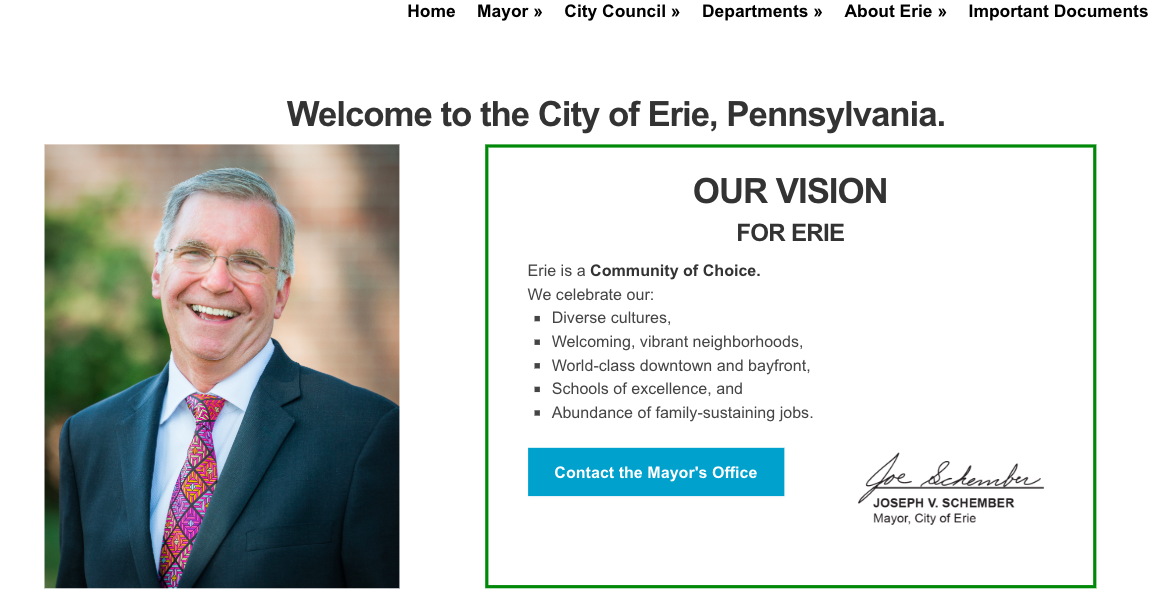
\includegraphics[scale=0.35]{figures/eriemayor}
\caption{Screenshot from the homepage at \url{http://www.erie.pa.us/}, accessed on 06/14/2018. Image depicts  Democratic mayor of Erie, PA, Joseph Schember.}
\label{fig:eriemayor}
\end{figure}


Members of the public visit municipal government websites for a wide variety of purposes \citet{sandoval2012government}, and with significant regularity. In a survey conducted among a random sample of citizens in the state of Georgia in 2000---nearly two decades ago---found that 25\% of internet users reported visiting a local government website in the previous twelve months \citep{thomas2003new}. Furthermore, the use of a local government website is associated with an individual's perspective on government. \citet{tolbert2006effects} find that users of local government websites are more likely to trust local governments, and hold other positive attitudes related to local and federal governments. Lastly, in a study of residents of Kansas City, Missouri, \citet{ho2017government} find that participants' perceived quality of the city website is strongly associated with their perceptions of the overall effectiveness of the City's communication with the public.

The existing research that uses scraped websites provides an indication of the theoretical value of empirical analysis of web contents produced by governments, public officials, and candidates for office. The most pertinent literature to our research is the e-governance literature, which focuses on the online presence of governments from a usability and public service point of view. For the most part, research in this category develops a classification scheme to rate websites in terms of accessibility, ease-of-use, and function, and then hand-codes a set of websites according to these criteria \citep[e.g., ][]{Urban2002,Armstrong2011,Feeney2017}. As an example, \cite{grimmelikhuijsen2012developing} study local government websites with the goal of uncovering how they aid the goal of transparency. To this end, they analyze a set of Dutch municipalities in which air quality had deteriorated. The authors test whether local governments provide citizens with information about potential complications and solutions associated with this issue. Like most e-government studies, however, this publication does not make any use of automated text analysis. Branching out of the topic of e-government service provision, \citet{mcnutt2010virtual} uses Canadian government websites to study how well-connected government websites are to non-profits and intergovernmental organizations in different public policy domains.
%Websites have also played a major role in the field of media studies, as scholars have scraped and analyzed the online presence of newspapers, as well as the more diffuse world of online political blogs \citep{Adamic2005,Gentzkow2010}. \cite{Lin2011} provide a good example of a study which makes extensive use of automated content analysis - a necessity arising from its dataset of 66830 blog posts and 57221 online news articles. The authors estimate the political slant of these entities by counting the frequencies with which politicians of either side are mentioned and determine that blogs are generally more biased. Unfortunately for us, the authors don't go into the details of their text analysis, and offer no information on the acquisition and pre-processing of the data.
%Another well-known example fitting into this area of study is the set of studies conducted by King et al. \citep{KING2013,King2014,KING2017}, in which the authors study censorship by the country's government on its lively blogosphere. However, the authors also provide no information on how their data was collected ``our extensive engineering effort, which we do not detail here for obvious reasons [...]''.

The websites of politicians and their parties have also been the object of research. Researchers have found that in order to identify the constituencies, motives, and modes of communication among these actors, their websites can be very illuminating sources of information \citep{Druckman2009,Druckman2010,Cryer2017,Esterling2011,Esterling2011a,Norris2003,Therriault2010}. \cite{Druckman2009,Druckman2010} rely on the \textit{National Journal} to find the websites, then hand-coded them. \cite{Cryer2017} mentions that she relied on Archive-it, a web service of the Internet Archive. Though the Internet Archive may provide extensive coverage of high profile officials or national governments, we found that its coverage of municipal government websites was sparse and irregular.
\cite{Esterling2011,Esterling2011a} rely on hand-coded data by the Congressional Management Foundation, a nonprofit organization which aims to assist Congress. \cite{Therriault2010} use automated text analysis, and also has the most extensive overview of the associated methodology. However, the division of the website into sections (home page, topics, issues, details) is done by hand. The author acquired the websites from the Library of Congress (which only collected them from legislators who actually consented, and Therriault notes that this causes nonrandom missingness).

Important to our methodological objectives, research analyzing and improving the scraping, pre-processing and text analysis pipeline that is applicable to government websites is still in its infancy. \cite{Eschenfelder2002} provide something of an overview of how federal websites should be assessed from an e-governance point of view, but they largely focus on the substantive criteria that should be fulfilled, rather than the technical aspects of website acquisition and analysis. %In what follows we first define the target dataset---the textual contents of websites of United States municipalities, along with associated metadata on the municipalities and their governments. We then define a pipeline for data collection and analysis that includes methods to access government website URLs, scrape their raw contents from the World Wide Web, gather plain text from the website files, and identify boilerplate text within the plain text contents. Lastly, we illustrate the analysis of municipal government website text by exploring the relationship between the city mayors' party affiliations and the topical contents of the websites.



\section{Data: US Municipal Government Website Text}

For data availability reasons, we focus our analysis of municipal websites on six states---Indiana, Louisiana, New York, Washington, California, and Texas. The selection of states and cities is largely dictated by the presence of partisan mayors and availability of the relevant data. Municipal elections in Indiana and Louisiana are partisan across the board,\footnote{In Indiana, this includes only cities - incorporated municipalities with at least 2,000 inhabitants - as opposed to towns.} so our sample is primarily focused on these two states. Here, all cities with a website are included, resulting in a considerably larger sample than for the other four states. New York and Washington do not have nominally partisan elections, but for a subset of cities, partisanship can be determined through contribution data (see below for more detail on how we use this data). Finally, California and Texas contain a number of large cities, whose mayors are sufficiently well-known for their partisanship to be available. These six states also provide us with a sample that is well-balanced on a number of theoretically important indicators. One, each of the four geographic regions are represented with at least one state. Two, we have a fairly well-balanced sample with respect to the urban/rural cleavage, as both major cities and less densely populated areas are covered. Furthermore, the sample is politically balanced---we have three blue states (CA, WA, NY) and three red states (TX, IN, LA). Finally, our dataset contains some of the wealthiest states (NY, CA, WA and TX are \#2, \#8, \#9 and \#16 respectively, by GDP per capita \citep{BureauofEconomicAnalysis2017}), but also some of the poorer ones (IN and LA). 

We acquired the website URLs from two sources: One, we scraped the URLs of city websites from their respective Wikipedia pages, which we found from lists of cities contained within each state. Two, the General Services Administration (GSA) maintains all `.gov' addresses, and provides a complete list of all such domains to the public.\footnote{The dataset is made available at \url{https://github.com/GSA/data/tree/gh-pages/dotgov-domains}. This list is updated once per month---we rely on the version released on January 16, 2017.} The data from the GSA contains the following variables: (1) domain name, specifically, the all-uppercase version of domain and top-level domain (for example, 'ABERDEENMD.GOV'); (2) the type of government entity to which the domain is registered, such as city, county, federal agency, etc; (3) for federal agencies, the name is specified; (4) the city in which the domain is registered. Naturally, the GSA's list does not contain cities which do not use a `.gov' website (or, in many cases, a city owns a registered `.gov' address, but uses a different one). Furthermore, some of the links are non-functional, and some of the county websites on the list are incorrectly marked as city websites (and vice versa). Since the GSA data is less complete and less reliable than the URLs found on Wikipedia, we mainly rely on the former and only supplement them with the GSA data if a specific city doesn't have a URL recorded on Wikipedia, or our tests (see below) find it to be non-functional.

Not all of the URLs contained in these archives are functional. To test the URLs' functionality, we use a web driver-controlled browser - a browser that is automatically controlled by a program rather than a human user. We use the Python bindings for the program \texttt{Selenium}, which we use to control \texttt{Firefox} through the web driver  \texttt{Geckodriver}. This is advantageous compared to conventional scraping tools such as \texttt{Beautiful Soup} or \texttt{Rvest} because most websites are designed to be explored by browsers. Modern browsers perform a lot of actions behind the scenes, such as URL resolution and redirection. The use of a web drive-controlled browser is necessary in our case because a) some city websites simply don't work, but they don't always output an error code correctly (this can fail, for example, if a webmaster simply stops maintaining a site without removing it entirely) which would throw off an automatic scraper, and more often, b) cities sometimes change their websites' URLs, in which case they redirect from the old to the new URL. A web driver-controlled browser, unlike the more rigid conventional scraping tools, will simply follow this redirection. This allows us to subsequently record and use the new URL for the actual website scraping. Consequently, an automated browser allows us to robustly answer the following questions: Is the website actually there? Does it work? If not, is it somewhere else or is it broken? We record this information and construct a list of verified URLs.

To download the websites, we rely on the Unix command line tool \texttt{wget}. This program is used to download files from the Internet, and with the use of a recursive option, acts like a web crawler and scraper. This means that \texttt{wget} downloads HTML files, parses them and then follows the links contained therein. Then it follows those links and repeats the process until it has constructed a complete tree of the website (note that the program is instructed to stay on the same domain, i.e. it does not follow external links). This way, all the files that make up a website are downloaded. For some cities, whose websites make heavy use of JavaScript to serve content dynamically, such content is not reachable with our methodology and would require additional steps to obtain. For this paper, we ignore such sites and restricted our corpus to cities with at least three successfully downloaded pages.\footnote{There is a possibility that this leads to a small bias in selecting against cities with the resources to build more elaborate websites. However, given that our sample is generally more on the wealthy side, this, if anything, should lead to a more balanced sample.}

The partisanship of the mayor of each city is coded in different ways, depending on the state. For Indiana, where elections are nominally partisan, this information is accessible through the state government's website\footnote{\url{http://www.in.gov/apps/sos/election/general/general2015?page=office&countyID=1&officeID=32&districtID=-1&candidate=}}. For Louisiana, we received data on the outcomes of mayoral elections from the Local Elections in America Project (LEAP) \citep{marschall2013local}. For the other states, where mayoral elections are not nominally partisan (but the partisanship of the mayor is still well-known), we employed different means: For New York and Washington, we searched the state campaign finance websites, and coded the parties of the candidates based on the party committees from which they received donations. For California and Texas, where our data consists of highly populated cities, partisanship information was acquired from Ballotpedia\footnote{\url{https://ballotpedia.org/List_of_current_mayors_of_the_top_100_cities_in_the_United_States}}. Finally, we also scraped mayoral partisanship from the cities' Wikipedia pages. When compared to the other data sources above, (and manual searches in case of conflicts) Wikipedia proved to be very reliable and added additional cases to our dataset even for Indiana and Louisiana. Generally speaking, we found data scraped from Wikipedia, aided by manual corrections in case of missing or conflicting data, to be more reliable than data from governmental sources. The partisan breakdown of city websites is depicted in Table \ref{tab:cityparties}. The dataset is has a relative party balance, with variation in each state.

% latex table generated in R 3.5.0 by xtable 1.8-2 package
% Wed Jul  4 14:14:10 2018
\begin{table}[ht]
\centering
\begin{tabular}{lrr}
  \hline
State & Democratic & Republican \\ 
  \hline
California &   9 &   6 \\ 
  Indiana &  46 &  54 \\ 
  Louisiana &  28 &  17 \\ 
  New York &  36 &  16 \\ 
  Texas &   2 &   7 \\ 
  Washington &  11 &   2 \\ 
   \hline
\end{tabular}
\caption{Descriptive statistics on the partisanship of the cities in the corpus.} 
\end{table}

 

One of the more subtle aspects of local government is the presence of different types of government structures. Between council-manager governments and mayor-council governments \citep{morgan1992policy}---either in the weak or strong mayor variant \citep{desantis2002city}---there is a certain degree of variance in where a city's executive authority lies. Unfortunately, we do not have access to information about the type of governments across the breadth of our dataset and therefore cannot explore heterogeneity in the relationship between mayoral partisanship and municipal website contents based on the executive system variant. Given the prominent place that mayors tend to have on their cities' websites, we feel that any bias arising from this nuance should be minor. \citep{gerber2011mayors}, whose model is somewhat comparable to ours in the sense that they also test the effect of mayoral partisanship on city policy priorities (on a sample of large cities, for which this information is more easily available), find that the inclusion of this potential confounder does not affect the results. Information on other covariates (population and median household income - from the American Community Survey 5) was acquired through the API of the U.S. Census Bureau\footnote{\url{https://www.census.gov/data/developers/data-sets.html}}.


\section{The Web to Text Pipeline}

Once we have gathered the website files, we have the raw data necessary for text analysis, but it is not yet formatted effectively. As is common in text analysis applications, we need to pre-process our data \citep{denny2018text}. In this section, we describe our pre-processing pipeline, with which we take an archive of website files, and output a corpus of formatted plain text files that are suitable for comparative analysis with text as data methods. In this pipeline, we address two methodological challenges. First, though they contain significant amounts of text, websites are not comprised of clean plain text files. Rather, the files available at websites are of multiple types, including HTML, PDF, word processor, plain text, and image files. The first step in the methodological pipeline is aimed simply at extracting clean plain text from this heterogeneous file base. The second step in our methodological pipeline is to process the text to remove boilerplate language---language that is effective at differentiating one website from another but is uninformative regarding policy or political differences between governments. Some of the steps we take in this processing pipeline are universally applicable in the analysis of textual data, and some of them are most appropriate for the particular type of text analysis that we apply to this data---statistical topic modeling. We will clarify this distinction as we describe steps in our pipeline.



\subsection{Site to Text Conversion}
The format of a file has a major impact on whether and how textual data can be extracted from a document. For all text analysis projects, researchers need to consider file formats. For the most part, the file type of a document can be correctly determined through the filename ending---its extension. However, there are exceptions to this, which, if ignored, can lead to large amounts of improperly formatted text, arising from incorrectly converted documents, which leads to a general decrease in the amount of usable data. Two issues, in particular, need to be addressed: One, HTML files on city websites frequently do not have an ending but are still perfectly readable if correctly identified as such. Second, some documents contain the incorrect file ending. For example, we found thousands of documents that ended in .html, when they were actually PDFs. To accurately assess their type, we rely on the R package \texttt{wand} \citep{wand}, which is an R interface to the Unix library \texttt{libmagic} \citep{darwin2008libmagic}, which determines the type of a file on the basis of its file signature - or ``magic number''. This short sequence of bytes at the start (and sometimes end) of files is unique for each file type and therefore allows its correct identification through computer forensics tools such as \texttt{libmagic}.

Consequently, we rename all documents so that their file ending reflects their actual file type. This is strictly necessary because we rely on the \texttt{readtext} R package \citep{readtext}, which determines a document's type solely through its ending---to convert the files to plain text.\footnote{We have also experimented with several Unix-based alternatives, but found that they largely led to the same results as \texttt{readtext}.} The breakdown of the files by type is given in Table \ref{tab:filetypes}. The most frequent file types are HTML and PDF, from which we are able to extract a substantial amount of usable text. Files of type XML, DOC, TXT, and DOCX, also occur regularly in our corpus and offer a considerable volume of textual data.



% latex table generated in R 3.4.4 by xtable 1.8-2 package
% Fri Jul 13 15:10:43 2018
\begin{table}[ht]
\centering
\begin{tabular}{lll}
  \hline
Filetype & Occurances After & Occurances After \\ 
  \hline
html & 211682 & 887362 \\ 
  pdf & 464842 & 638802 \\ 
  jpg & 0 & 36958 \\ 
  xml & 0 & 29638 \\ 
  Other & 162681 & 9475 \\ 
  ics & 435 & 8950 \\ 
  png & 0 & 8863 \\ 
  doc & 6972 & 8430 \\ 
  txt & 317 & 6025 \\ 
   & 793990 & 5234 \\ 
  docx & 3137 & 4319 \\ 
  TOTAL & 1644056 & 1644056 \\ 
   \hline
\end{tabular}
\caption{Number of files per type, before and after detecing them via their magic number. The table shows that a lot of files originally have the wrong type, and that converting them correctly has a large impact on how many of them end up being usable.}
\label{tab:filetypes} 
\end{table}




We then take several steps to pre-process the data as required for the subsequent analysis. Pre-processing choices should be contingent on the analysis being conducted with the text later and can have significant effects on the outcomes of an analysis \citep{denny2018text}. The type of text analysis we conduct---topic modeling---requires that the words in the document be meaningful and interpretable, and does not make use of the sequence of words within a document (i.e., is a bag-of-words method). %With the exception of file type conversion and boilerplate removal, the pre-processing steps taken here should therefore not be seen as universally applicable to all analyses of government website data.

The text documents are converted to UTF-8 character encoding and then stripped of dates, punctuation, numbers, and words connected by underscores. At this point, the documents of one city still closely resemble one another in the form of boilerplate content, be it website elements (i.e. "You are here", "Home", "Directory" etc.) in HTML documents, or commonly used forms or phrases in pdf, doc and docx files. This is an issue, because this boilerplate content causes the results of analyzing this data with text analysis methods to characterize documents primarily by the cities from which they originate (through their unique boilerplate structure, e.g. a menu with certain terms repeated on every site of the domain), and not the substantive features of their contents. Boilerplate removal is a useful step in many forms of text analysis, as the analysis is focused in on text that varies above and beyond a standard template for textual content. Our solution to this problem is described in more detail in Section \ref{boilerplate}.

The last round of preprocessing is intended to remove everything from the file that is not an English word. This step is tailored to our intention to use the text for topic modeling. The final preprocessing round includes setting every character to lowercase, as well as the removal of bullet points which frequently occur in HTML documents, extraneous whitespace, XML documents mislabeled as HTML files, and empty documents. Furthermore, some documents contain gibberish, often as a result of faulty or impartial optical character recognition applied to text that was produced through a non-machine-readable medium. To combat this problem, we employ two solutions. One, we use spellchecking, implemented through the \texttt{hunspell} R package \citep{hunspell}, to remove all non-English words.\footnote{Some of the cities, for example, Los Angeles, do contain a sizable proportion of Spanish content. The analysis of this content is beyond the scope of this paper but could be explored in future work, for example using methods of text processing that are applicable to multilingual corpora \citep{lucas2015computer}. } However, \texttt{hunspell} does not cover everything, either because some tokens are not actual words (for example artifacts from defective encoding), or because random sequences of characters just so happen to form words that exist in a dictionary (for example "eh" or "duh"). Since we rely on a bag-of-words model in which syntax does not matter, we can ameliorate these problems by removing all text except for whitespaces and the characters that appear in the English alphabet. Since a lot of the nonsensical text tends to be quite repetitive, we also delete all documents in which the proportion of unique to the total number of tokens is less than 0.15. Furthermore, \texttt{hunspell} does not spellcheck individual characters or two-character words, so we remove these token types entirely. Since these pre-processing steps reduce documents which are largely unsuitable to only a few tokens (i.e., word occurrences), we also remove all remaining documents containing less than 50 tokens. Finally, to remove words that are extremely rare (which also has the advantage of eliminating any remaining oddities) and thus add nothing substantive\footnote{Topic models essentially do not pick up on extremely rare words, so their inclusion is a waste of computational resources. Removing them in this manner is also the default preprocessing choice in the \texttt{stm} package.} to our models while increasing their computational cost, we also discard any token types that occur in only one document. We also conduct lemmatization to reduce words to their basic form. Lemmatization is similar to stemming but works in a somewhat more sophisticated manner by taking grammar and surrounding words into account to identify the dictionary form of a word. For example, the lemma of the word ``lemmatization'' would be ``lemmatize'', whereas most stemmers would simply chop off the ending, which would yield ``lemmatiz''. Thus, lemmatization makes the results more easily comprehensible. To this end, we rely on the R package \texttt{spacyr}, which provides an R implementation of the Python library \texttt{spaCy}.

\subsection{Boilerplate Removal}\label{boilerplate}
As noted above, city websites contain a large amount of text that is uninformative for its actual content, and therefore a hindrance to understanding through algorithmic text analysis. This is a common issue with textual data in which informative content is embedded in technically structured documents. See, e.g., \citet{burgess2016legislative,wilkerson2015tracing} and \citet{linder2018text} for examples of boilerplate removal in the analysis of legislative text. In the case of websites, lines in documents are generally quite informative, so all of our boilerplate removal efforts are done at the line level.

%this is outdated; not deleting it yet in case we need it for further reference
%Consequently we remove this content as follows: Each line of every document is compared to every line in every other document belonging to the same city. We count how many times each line is duplicated for that city. We remove any line occurring more than our chosen threshold of 10.\footnote{Empirically, lines tend to be duplicated either hundreds of times or only once or twice, if at all.} This means that each document only retains the information that is particular about it. We implement this algorithm through hash tables, which reduces the computational complexity from O($N^2$) to O($N$). Before this step is taken, we remove numbers and dates from the documents because they frequently make lines unique, despite the fact that they are virtually the same (for example different days on a city calendar).

\subsection*{Boilerplate Classification}
In order to determine whether a line should be discarded, we train a classifier on a human-coded sample. We sampled 500 lines from documents in each of the following five cities: Los Angeles, CA, Indianapolis, IN, New York, NY, Shreveport, LA, and Seattle, WA. To ensure that lines which occur more frequently in these cities (sometimes hundreds of thousands of times) had a higher probability of being scrutinized by the classifier, we use sampling weights equivalent to the proportion of total lines in a city's corpus made up by each specific line type. As an example, the most common line throughout all pages of the city of Seattle consists only of the word ``total'' and occurs 103,068 times. Similarly, the line ``page'' occurs 58,833 times. Even something completely nonsensical such as ``a a'' still appears on 376 occasions. To account for the higher likelihood of some lines being part of the training set, we use inverse probability weights in training the classifier---the weight of each line in the sample is 1/[number of occurrences in the corpus].\footnote{Note that the performance of the classifier is robust to the use of these weights and only changes by about one percentage point if they are not used.}

These 500 lines were then hand-coded as either substantively informative (210 lines) or not (290 lines). We then trained a number of different classifiers with this informativeness measure as the dependent variable. The independent variables we use are: (1) number of times the line was duplicated within the city, (2) the length of the line, in characters, (3) the number of tokens in the line, and (4) the median distance from the document midpoint to the position of the line itself. The purpose of these covariates is as follows:

\begin{itemize}
\item {\bf Line length:} The length of the line and the number of tokens are ways to find lines consisting of only a word or two. This is highly predictive of lines which are used as website headers and navigational elements, which are of zero substantive interest to us but are very effective at differentiating cities. These terms also happen to be fairly common, which causes them to be overweighted by the topic model.

\item {\bf Number of line duplications:} To directly address the latter problem, we include a measure of the number of times a line is duplicated within a city. Many lines occur hundreds or even thousands of times on a single website and therefore are terms that are highly predictive of the website, which causes the topic model to find topics that are highly predictive of cities, but not substantively informative.

\item {\bf Line position in the document} Since boilerplate terms such as navigational elements, headers, footers, and so on, should occur more frequently at the beginning and the end of websites, we attempt to identify such content as following: We measure the distance between the midpoint of a document and the position of a line, expressed as quantiles (to account for differing document lengths). Since lines can occur in multiple documents or multiple times in the same document, we take the median of these measures. Thus, for example, a line which often occurs at the beginning of documents might have a score of 0.45, whereas a line that tends to be found more in the center, and thus is indicative of more relevant content, might be scored with a 0.11 instead.
\end{itemize}


%Finally, the keyness measure: This indicator shows whether a term occurs disproportionally frequently in one document collection, compared to another. In our case, this would be one city's documents, compared to all others. Mathematically, this is a simple chi-square test, asserting whether the frequency of a word in a city is greater than its expected count, as determined by its count in all other documents, and the number of tokens in the city. The variable used in the model is the chi-square value of this test for each word (which varies and is therefore calculated individually for each city).\footnote{Or alternatively, the log of the absolute chi-square value, after which the previously negative values are made negative again.}

%A regression table for this model can be found in table 3. The associated accuracy in 5-fold cross-validation is 0.8325. The cross-validation accuracy of a simplified model with only the number of characters as a covariate is 0.825 (table 4). A model with the four covariates described above as well as interaction terms between each of them yields an accuracy of 0.885 (table 5).

%
% Table created by stargazer v.5.2 by Marek Hlavac, Harvard University. E-mail: hlavac at fas.harvard.edu
% Date and time: Wed, May 23, 2018 - 03:39:09 PM
\begin{table}[!htbp] \centering 
  \caption{} 
  \label{} 
\begin{tabular}{@{\extracolsep{5pt}}lc} 
\\[-1.8ex]\hline 
\hline \\[-1.8ex] 
 & \multicolumn{1}{c}{\textit{Dependent variable:}} \\ 
\cline{2-2} 
\\[-1.8ex] & class \\ 
\hline \\[-1.8ex] 
 nchars & $-$0.003 \\ 
  & (0.002) \\ 
  & \\ 
 nwords & $-$0.018 \\ 
  & (0.013) \\ 
  & \\ 
 medianDocMidDist & 0.056 \\ 
  & (0.158) \\ 
  & \\ 
 prob & 8.515$^{**}$ \\ 
  & (3.856) \\ 
  & \\ 
 freq & $-$0.00000 \\ 
  & (0.00000) \\ 
  & \\ 
 Constant & 0.813$^{***}$ \\ 
  & (0.048) \\ 
  & \\ 
\hline \\[-1.8ex] 
Percent Correctly Predicted & 0.844 \\ 
Precision & 0.795 \\ 
Recall & 0.978 \\ 
F1-Score & 0.876 \\ 
Observations & 400 \\ 
Log Likelihood & $-$193.686 \\ 
Akaike Inf. Crit. & 399.372 \\ 
\hline 
\hline \\[-1.8ex] 
\textit{Note:}  & \multicolumn{1}{r}{$^{*}$p$<$0.1; $^{**}$p$<$0.05; $^{***}$p$<$0.01} \\ 
\end{tabular} 
\end{table} 

% latex table generated in R 3.4.4 by xtable 1.8-2 package
% Sat Jul 28 20:34:44 2018
\begin{table}[ht]
\centering
\begin{tabular}{rr}
  \hline
 & Value \\ 
  \hline
Percent Correctly Predicted & 0.87 \\ 
  Precision & 0.87 \\ 
  Recall & 0.91 \\ 
  F1-Score & 0.89 \\ 
   \hline
\end{tabular}
\caption{Performance metrics for random forest boilerplate classifier, with inverse probability weights.} 
\label{randomForest}
\end{table}


%% latex table generated in R 3.4.4 by xtable 1.8-2 package
% Sat Jul 28 20:34:45 2018
\begin{table}[ht]
\centering
\begin{tabular}{lr}
  \hline
Feature & Importance \\ 
  \hline
nchars & 100.00 \\ 
  nwords & 83.70 \\ 
  medianDocMidDist & 13.50 \\ 
  freq & 0.00 \\ 
   \hline
\end{tabular}
\caption{Variable importance for random forest boilerplate classifier, with IPW weighting.} 
\label{randomForestVarimp}
\end{table}



We rely on a random forest as the final classifier, which offers slightly better performance than logistic regression.\footnote{We also tried SVM, boosted trees and AdaBoost, with similar results and chose the random forests because this method has a probabilistic basis and is more intuitive.} We assess the performance of this classifier through five-fold cross-validation. This means that the classifier is trained on 400 samples and then tested on the held-out set of 100, measuring metrics such as percent correctly predicted, precision, recall, and F1 score. This procedure is carried out five times so that each sample is part of the test set once. The aggregated (mean) results of this process can be found in Table \ref{randomForest}. For the implementation of this method, we rely on the R package \texttt{caret}, whose random forest classifier is based on the package \texttt{ranger}. We use this classifier to flag and remove all lines that are not classified (based on a threshold of $p = 0.5$) as substantively meaningful. The effect of this process on the corpus is illustrated with the corpus of Anchorage, AK (i.e. a city that isn't part of our sample used in the analysis) as an example in Figures \ref{boilerplate_before_after1} to \ref{boilerplate_before_after4}. Before the lines identified by the classifier as boilerplate are removed, lines with very few characters and words are the most common. After the removal, the distribution has changed---lines of medium length now occur more frequently than extremely short ones, which are unlikely to be substantively meaningful (see figures \ref{boilerplate_before_after1} and \ref{boilerplate_before_after2}). Furthermore, lines that are duplicated only a few times rather than dozens, hundreds or even thousands are now more common (see figure \ref{boilerplate_before_after3}). Finally, the position of the line in the documents is not as important to the random forest, and this also shows in the results. However, this feature still has a positive effect, as lines at either end of the document are a bit less common now (see figure \ref{boilerplate_before_after4}). Table \ref{tabBoilerplateIllustration} provides further illustration by listing the top 10 most likely boilerplate lines (in Anchorage, AK) -- all of which were flagged as such with a probability of 1. After all the preprocessing is set and done, our corpus consists of 259,099 documents.

\begin{figure}[htp]
    \centering
    \caption{Effects of the boilerplate classifier on the corpus of the city of Anchorage, AK. After the boilerplate content is removed, extremely short lines are less common.}
    \label{boilerplate_before_after1}
    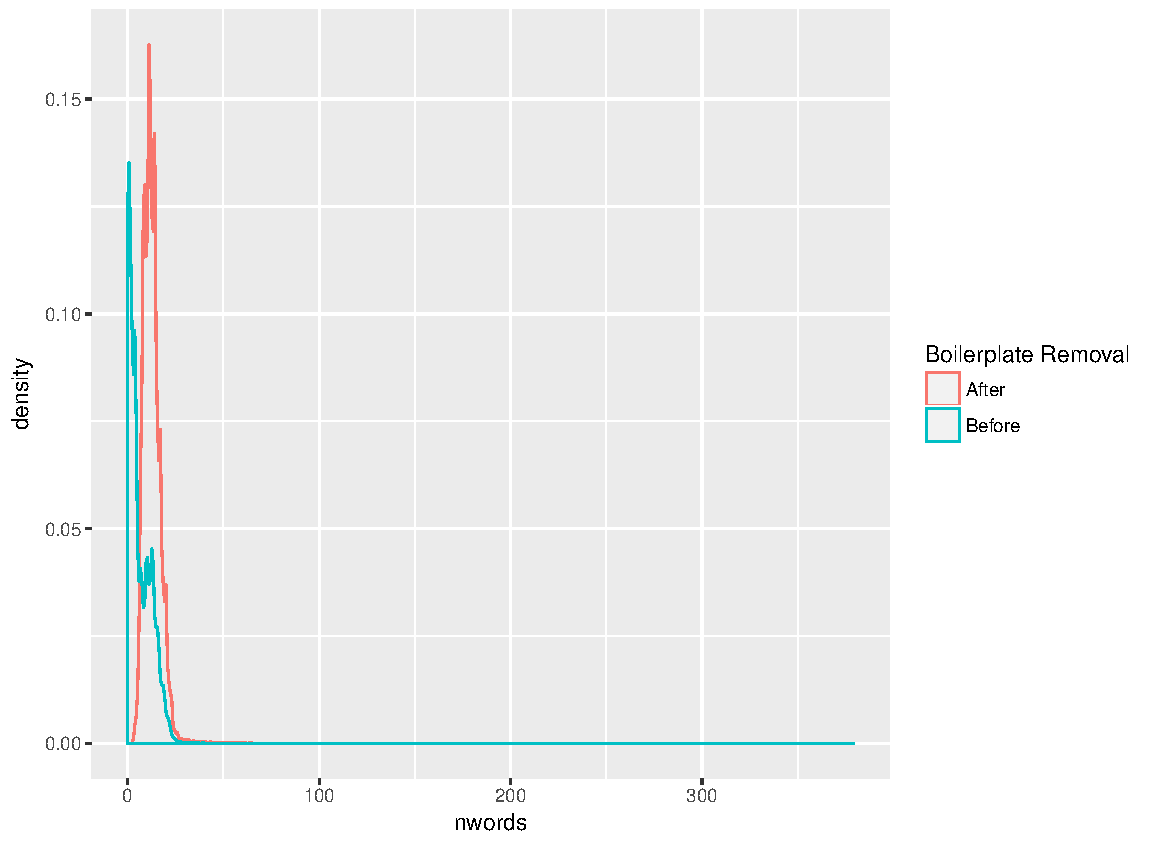
\includegraphics[width=\linewidth]{figures/boilerplateBeforeAfterNwords.pdf}
\end{figure}
\begin{figure}[htp]
    \centering
    \caption{Effects of the boilerplate classifier on the corpus of the city of Anchorage, AK. After the boilerplate content is removed, extremely short lines are less common.}
    \label{boilerplate_before_after2}
    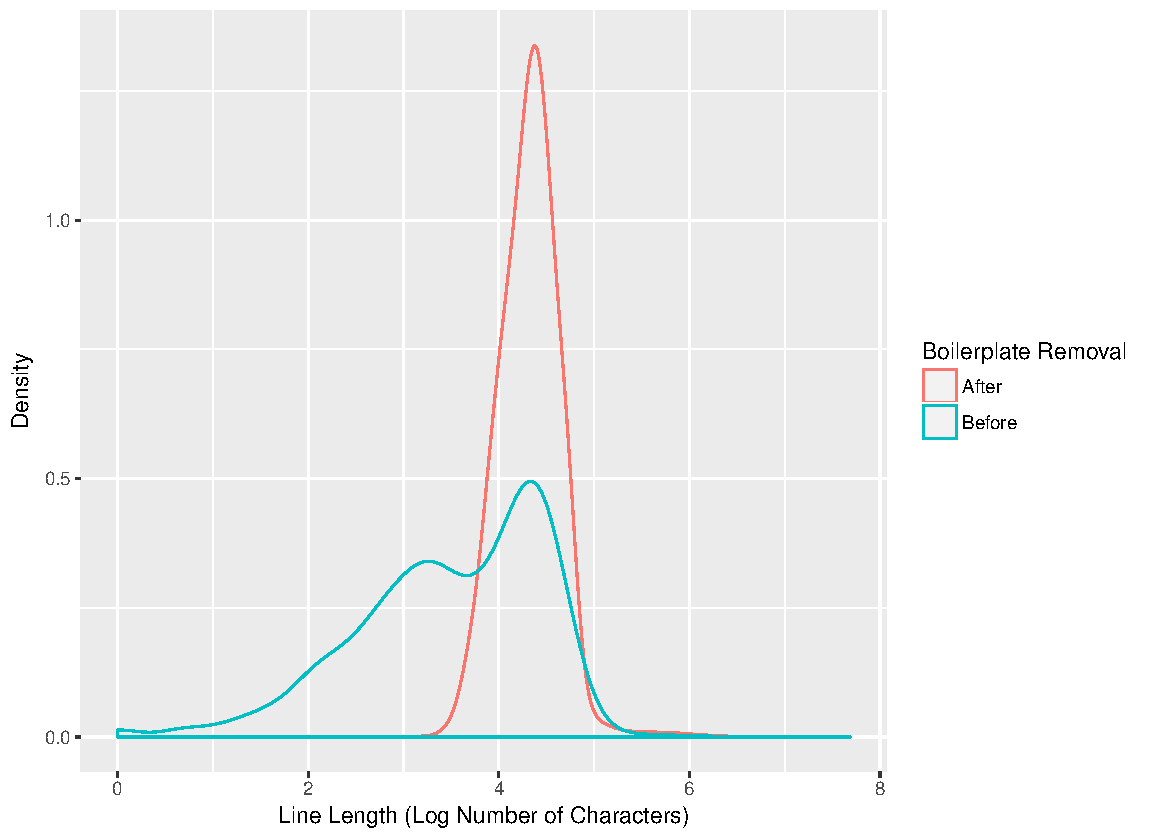
\includegraphics[width=\linewidth]{figures/boilerplateBeforeAfterNchars.pdf}
\end{figure}
\begin{figure}[htp]
    \centering
    \caption{Effects of the boilerplate classifier on the corpus of the city of Anchorage, AK. After the boilerplate content is removed, lines that are duplicated hundreds or thousands of times are less common.}
    \label{boilerplate_before_after3}
    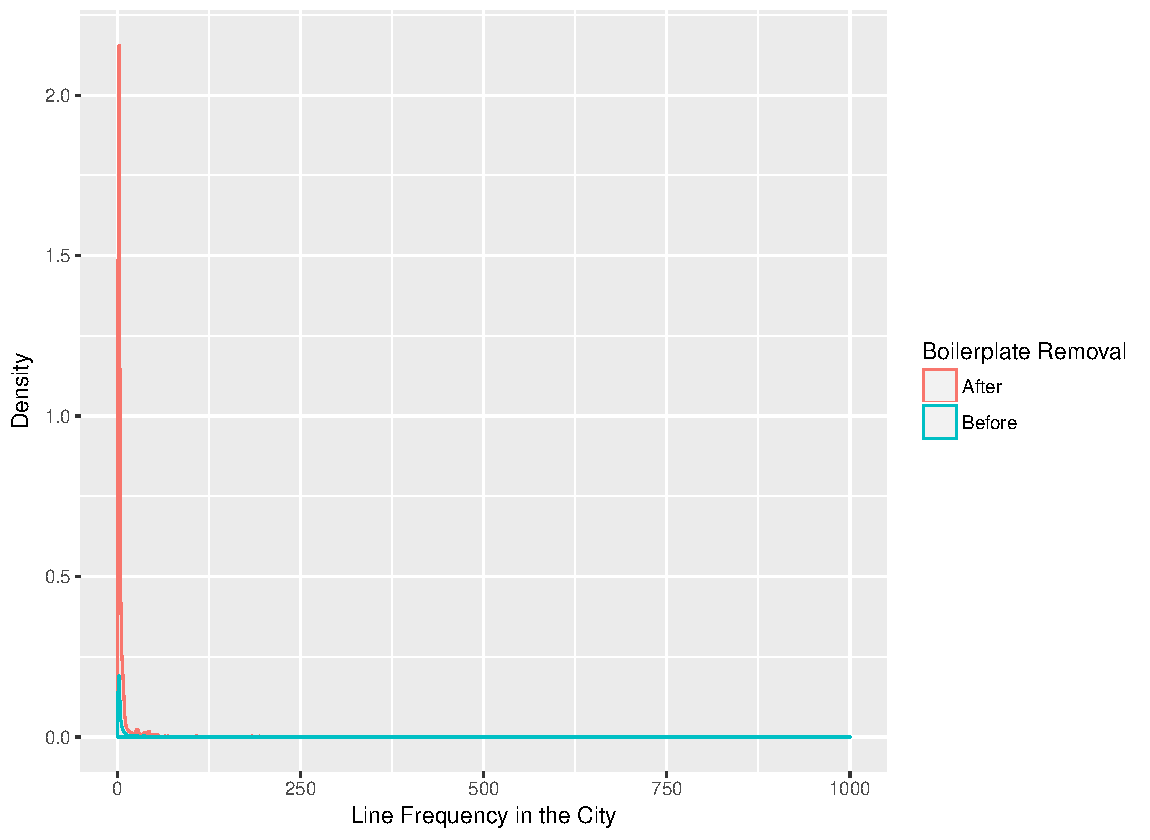
\includegraphics[width=\linewidth]{figures/boilerplateBeforeAfterFreq.pdf}
\end{figure}
\begin{figure}[htp]
    \centering
    \caption{Effects of the boilerplate classifier on the corpus of the city of Anchorage, AK. After the boilerplate content is removed, lines at the beginning and end of documents are less common.}
    \label{boilerplate_before_after4}
    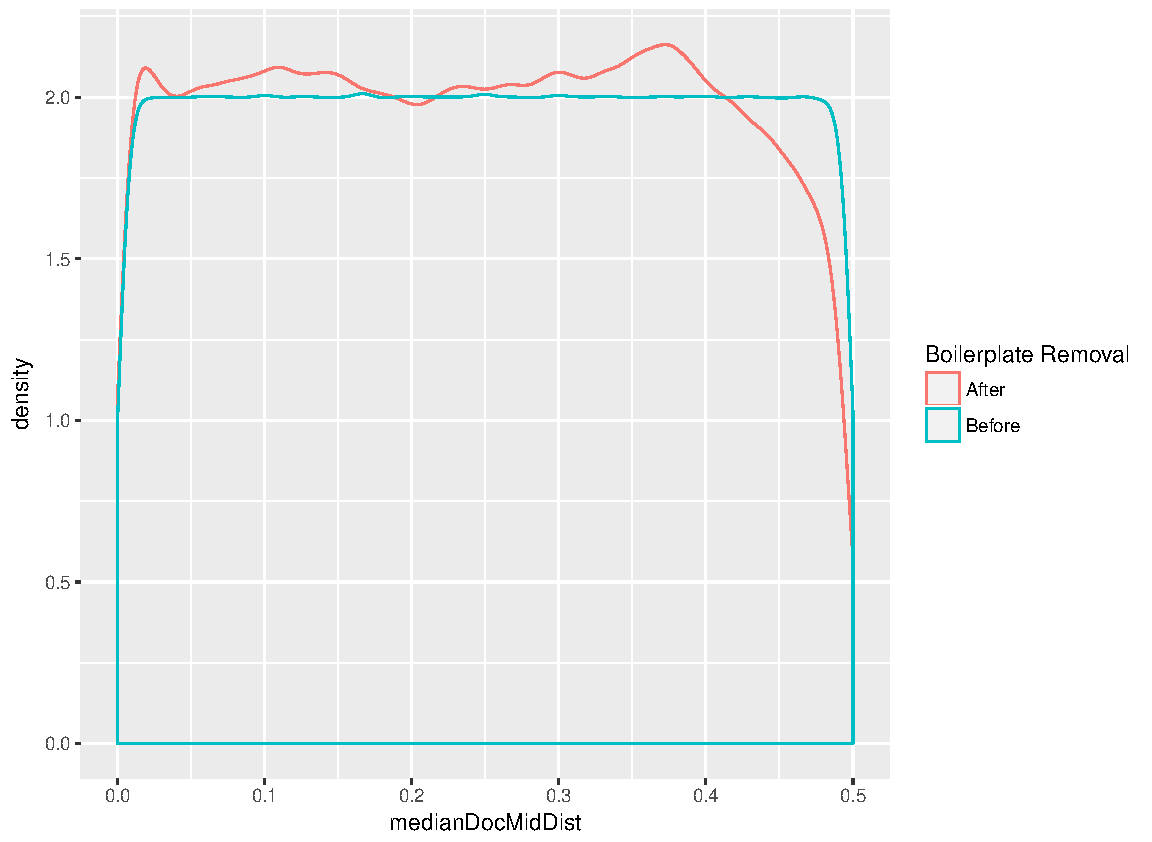
\includegraphics[width=\linewidth]{figures/boilerplateBeforeAfterMedianDocMidDist.pdf}
\end{figure}

\section{Partisan Language on Municipal Websites}

We illustrate the analysis of municipal website content by studying differences in website content based on the party of the mayor. As we reviewed above, the partisanship of the mayor has been found in past research to affect several features of city governance. However, \citet{gerber2011mayors} note that, due to the constraints of state and national policies, municipalities lack discretion in many domains of governance. They find that cities with Democratic mayors spend a smaller share of their budgets on public safety, but that mayoral partisanship does not appear to be significantly related to spending in most other areas, where cities have less discretion. As opposed to budget allocation or even the presence/absence of policies, cities have a great deal of discretion regarding what is emphasized on their websites, and how policies are framed. Since (1) city governments have great discretion in composing their websites, (2) modifying website content is low cost relative to other policy changes, and (3), as reviewed above, city websites provide an effective and often-used means of communication with city residents.

%BoW methods are methods of text analysis that do not take into account the sequence or placement of words in text---just the presence and frequency of words. As noted by \cite{GrimmerStewart2013}, for most applications, bag-of-words approaches have been found to be more than sufficient. Furthermore, there is reason to believe that city government websites are a particularly `safe' case for bag-of-words methods due to their informative, manner-of-fact based language. It is extremely unlikely for these pages to feature ambiguous language such as an abundance of negation or even sarcasm.


% latex table generated in R 3.4.4 by xtable 1.8-2 package
% Fri Aug 10 15:55:53 2018
\begin{table}[ht]
\centering
\begingroup\small
\begin{tabular}{lrr}
  \hline
Line & Substantive & Boilerplate \\ 
  \hline
have questions & 0.00 & 1.00 \\ 
  stay connected & 0.00 & 1.00 \\ 
  accident or injury & 0.00 & 1.00 \\ 
  fire damaged buildings & 0.00 & 1.00 \\ 
  gas connections & 0.00 & 1.00 \\ 
  harboring of vagrants & 0.00 & 1.00 \\ 
  roof system problem & 0.00 & 1.00 \\ 
  violation plat note & 0.00 & 1.00 \\ 
  violation setback & 0.00 & 1.00 \\ 
  violation site plan & 0.00 & 1.00 \\ 
   \hline
\end{tabular}
\endgroup
\caption{Lines (or the first 50 characters of a line) in the corpus of Anchorage, AK, with the 10 highest probabilities of being classified as boilerplate.} 
\label{tabBoilerplateIllustration}
\end{table}



\subsubsection{Analytical approach: Structural topic modeling}
In order to analyze content differences between government websites based on mayoral partisanship, we draw upon a recently-developed class of text-as-data methods, the structural topic model, developed by \citet{Roberts2014}. Building on the conception of ``topics'' in Latent Dirichlet Allocation, in the structural topic model a topic is a multinomial distribution defined on the word types in the dictionary.  Each word occurrence in a document is attributed with a single topic label. The word topic assignments are also drawn from a multinomial distribution. The log-odds of the topic probabilities in each document-specific multinomial distribution over topics are drawn from a multivariate normal distribution in which the topic-specific means are determined by a linear regression function that associates document-attributed covariates with topics. For example, in the context of municipal website content, the structural topic model can be used to estimate a regression coefficient that defines the linear relationship between the log-odds of the municipality's population and the log-odds of each topic. For our primary empirical investigation, the structural topic model provides with a tool with which to estimate the relationship between the party of the city's mayor and the prevalence of each topic we estimate. A topic interpreted through post-hoc analysis of the collective meaning of the most likely words to be drawn from the multinomial distribution defined by the respective topic.\footnote{The ``Fightin' Words'' methodology developed by \citet{Monroe2008} could also be used to analyze word-frequency differences between cities based on mayors' partisanship, but we elected to use the structural topic model since, unlike ``Fightin' Words'' , the structural topic model enables us to adjust for several other features through multiple regression.}

The structural topic model is implemented in the R package \texttt{STM} \citep{stm}. We use 60 topics---the number recommended by the authors\footnote{For this recommendation, see the documentation for the function \texttt{stm()} in version 1.3.0 of the R package \texttt{stm} \citep{stm}.} for medium- to large-sized corpora. Since our corpus is at the larger end of that spectrum, the appendix also contains the results of a model with 120 topics, which corroborates the findings of the one presented here. We use four covariates: First, \textit{party}, to estimate the difference in topic prevalence based on whether mayors are Republican or Democratic. Second, \textit{city population}, which the literature frequently emphasizes as a determinant of the issues a city faces (see, for example, \cite{Guillamon2013}). Third, we control for wealth by relying on \textit{median income} as a covariate, which we use as a proxy for the tax base in a city. Fourth and finally, we include state dummy variables, which should account for language that is associated with state-specific issues, and general background variables that vary across states.

\subsubsection{Structural topic model results}


The results are shown in Table \ref{tabSTMtopwords60}. The rows of the table are sorted so that the most Republican topics (marked by a deeper red color) appear at the top, and the most Democratic ones (blue) at the bottom. The degree of partisanship shown in the table is determined by the size and direction of the coefficient of the party variable for each topic. The topics that are entirely white have 90\% credible intervals on the effect of the mayoral party that include zero.

Many of the topics associated with Democrats fit with what we understand to be national party priorities. Topic 21, on affordable housing, clearly resonates with the Democratic party's appeal to low-income voters. Similarly, employee rights are represented in Topic 47. Democrats also exhibit a strong preference for words related to public finances, such as Topic 32 ('budget', 'revenue', 'expenditure') as well as Topic 19 ('debt', 'bond', 'financial'). We suspect that the association of Democratic mayors with finance-related terms is indicative of a greater willingness to emphasize the city's efforts to raise and spend money. This finding is consistent with \citep{Einstein2015}, who show that Democratic mayors tend to favor greater spending. A second, consistent Democratic focus appears to be law enforcement: The most Democratic topic, 55 ('robbery', 'homicide', 'sergeant') (a comparable topic is also the most Democratic topic in the model with 120 topics in tables \ref{tabSTMtopwords120_1} and \ref{tabSTMtopwords120_2} of the Appendix) depicts Democrats' complicated relationship with law enforcement. On the one hand, Democratic partisans have a more negative perception of the police, rating it considerably more negatively on the appropriate use of force and the equal treatment of minorities \citep{Brown2017}. On the other hand, the literature has also shown that cities with a higher Democratic vote share spend more on the police, even after controlling for crime \citep{Einstein2015}. Finally, Democrats also focus more on the deliberative process of policymaking, as topics 31 ('agenda', 'committee'), 34 ( `comment', `draft', `feedback'), 48 (`absent', `aye', `nay'), and 37 ('audit', 'procedure', 'oversight') attest to.  This openness regarding the policy process on behalf of cities with Democratic mayors fits with the findings of \citet{grimmelikhuijsen2012developing}, which are that left-wing local governments exhibit greater transparency via website content.

City websites with Republican mayors, meanwhile, exhibit a pronounced focus on the essential functions of government. Basic utilities such as energy (Topic 7), fire protection (Topic 17), drinking water (53), and garbage removal (Topic 49) are included among those topics that are more prevalent in cities with Democratic mayors. Similarly, protecting citizens from natural disasters is a focus in topics 1 ('storm', 'runoff', 'drainage') and 42 ('breastfeed', 'infection', 'mosquito' -- and so, essentially, about the Zika virus), which may reflect the greater prevalence of Republican mayors in the southeast, a region which is more often affected by hurricanes and tropical diseases.



%Interestingly enough, Democrats also `own' the topic related to law enforcement, which might be somewhat unexpected given Republicans' usual focus on law and order \citep{gerber2011mayors}. However, this kind of finding is not entirely without precedent in the literature (see \citep{Einstein2015}). Similar to the informed dirichlet model, the structural topic model also finds the emphasis on construction and infrastructure by Republicans - in table \ref{tabSTMINRep}, topics 2, 7 and 8 clearly focus on these issues.\footnote{The first Republican topic in Indiana (library, stream, obj, etc.) is likely an artifact from incorrectly converted HTML, and since it presumably only happens only in one Republican city, the topic is classified as very Republican.}

%When comparing Indiana to Louisiana, it appears that the Democratic emphasis on law enforcement is robust. Furthermore, as with the fightin' words approach, some smaller degree of focus on money (see topic 1) is still evident. For Republicans, topics 2 to 4 seem to be, once again about infrastructure and utilities, pointing to a certain degree of robustness in these results, as well as the emergence of a trend. The results produced by the structural topic model are not flawless, but the two parties do seem to have somewhat consistent themes on which they focus on in both states. Furthermore, in comparison to the fightin' words approach, the ability of the structural topic model to form coherent topics is quite evident and helpful in the interpretation of the results.

%An ostensibly intuitive solution to topics clustering into cities in LDA is to include dummies for the cities in a statistical model of topics. This is facilitated by the structural topic model, which uses document metadata t to account for variation in topics \citep{Roberts2014}. However, figure \ref{stm_results} shows that if anything, the STM exacerbates the problem. Here, we plot the \textit{p-values} of the coefficients for each city as well as the party variable across each topic. Under normal circumstances, plotting the p-values, as opposed to the fitted values, does not make much sense, but here it serves a diagnostic purpose. The plot shows that the party variable is never statistically significant at any conceivable level of confidence, nor is it even close to. Interestingly the same is true for a number of the cities as well. The topics cluster heavily into only about half of the cities, which does not present an improvement over LDA at all.

%Partisan top words - stm Louisiana -- Rep
%% latex table generated in R 3.4.2 by xtable 1.8-2 package
% Mon Nov 13 15:36:58 2017
\begin{table}[ht]
\centering
\begin{tabular}{llllll}
  \hline
0.024 & 0.019 & 0.019 & 0.016 & 0.016 & 0.016 \\ 
  \hline
motion & plan & inc & request & council & \cellcolor{red!25} traffic \\ 
  second & \cellcolor{red!25} zone & electr & board & citi & amp \\ 
  made & applic & build & member & ordin & vehicl \\ 
  approv & \cellcolor{red!25} properti & construct & servic & common & stop \\ 
  mayor & approv & home & \cellcolor{red!25} street & councilor & sign \\ 
  present & sign & street & approv & amend & \cellcolor{red!25} road \\ 
  state & \cellcolor{red!25} site & meridian & purchas & resolut & block \\ 
  will & locat & servic & citi & adopt & signal \\ 
  citi & commiss & west & move & wherea & \cellcolor{red!25} street \\ 
  council & file & main & good & approv & driver \\ 
   \hline
\end{tabular}
%\caption{Top Republican topics and words (Indiana), according to STM. 
%The words are the top words for the most Democratic/Republican topic, determined
%by the size (and significance) of the coefficient (see table header) of the party covariate.} 
\label{tabSTMINRep}
\end{table}

 %\ref{tabSTMINRep}

%Partisan top words - stm Louisiana -- Dem
%% latex table generated in R 3.4.3 by xtable 1.8-2 package
% Tue Dec 26 20:59:22 2017
\begin{table}[ht]
\centering
\scriptsize
\begin{tabular}{llllll}
  \hline
-0.027 & -0.022 & -0.016 & -0.011 & -0.011 & -0.01 \\ 
  \hline
city & school & downtown & city & \cellcolor{blue!25}trash & \cellcolor{blue!25}housing \\ 
  ordinance & community & business & department & city & property \\ 
  approve & program & project & mayor & \cellcolor{blue!25}waste & program \\ 
  resolution & student & city & police & day & \cellcolor{blue!25}fund \\ 
  property & \cellcolor{blue!25}education & \cellcolor{blue!25}development & officer & \cellcolor{blue!25}recycle & home \\ 
  purchase & \cellcolor{blue!25}university & new & public & street & city \\ 
  area & national & center & citizen & collection & project \\ 
  department & award & \cellcolor{blue!25}economic & work & resident & neighborhood \\ 
  contract & high & company & safety & \cellcolor{blue!25}recycling & \cellcolor{blue!25}grant \\ 
  service & year & community & resident & snow & unit \\ 
   \hline
\end{tabular}
\caption{Top Democratic topics and words}%\caption{Top Democratic topics and words (Indiana), according to STM. 
%The words are the top words for the most Democratic/Republican topic, determined
%by the size (and significance) of the coefficient (see table header) of the party covariate.} 
\label{tabSTMINDem}
\end{table}

 %\ref{tabSTMLADem}

%Partisan top words - stm Louisiana -- Rep
%% latex table generated in R 3.4.3 by xtable 1.8-2 package
% Tue Dec 26 15:50:18 2017
\begin{table}[ht]
\centering
\begin{tabular}{llllllll}
  \hline
0.071 & 0.054 & 0.054 & 0.034 & 0.033 & 0.024 & 0.023 & 0.02 \\ 
  \hline
event & ordinance & water & street & say & city & city & mayor \\ 
  information & department & emergency & traffic & can & business & meeting & city \\ 
  show & summary & city & parking & make & new & council & parish \\ 
  park & amount & resident & lane & get & mayor & commission & town \\ 
  music & bid & storm & project & take & development & plan & office \\ 
  food & city & weather & work & people & economic & member & hall \\ 
  visit & public & waste & bike & work & million & public & contact \\ 
  weekend & police & system & downtown & need & continue & board & day \\ 
  festival & approve & power & public & city & work & committee & official \\ 
  begin & inc & service & bicycle & help & local & planning & state \\ 
   \hline
\end{tabular}
\caption{Top Republican topics and words (Louisiana), according to STM. 
The words are the top words for the most Democratic/Republican topic, determined
by the size (and significance) of the coefficient (see table header) of the party covariate.} 
\label{tabSTMLARep}
\end{table}

 %\ref{tabSTMLARep}

%Partisan top words - stm Louisiana -- Dem
%% latex table generated in R 3.4.3 by xtable 1.8-2 package
% Mon Dec 25 01:20:56 2017
\begin{table}[ht]
\centering
\begin{tabular}{llllllll}
  \hline
-0.044 & -0.04 & -0.021 & -0.019 & -0.016 & -0.012 & -0.011 & -0.01 \\ 
  \hline
owner & provide & victim & application & employee & city & revenue & community \\ 
  applicant & otherwise & crime & motion & policy & ordinance & fund & neighborhood \\ 
  new & respect & violence & second & city & whereas & tax & district \\ 
  application & thereto & arrest & street & report & bond & budget & police \\ 
  per & city & domestic & favor & department & resolution & million & public \\ 
  exist & authorize & officer & retention & audit & code & total & meeting \\ 
  build & ordinance & suspect & john & review & provide & year & engagement \\ 
  proposal & amend & report & arc & management & shall & general & crime \\ 
  receive & district & child & window & procedure & provision & service & officer \\ 
  construction & locate & police & heather & work & fund & forecast & department \\ 
   \hline
\end{tabular}
\caption{Top Democratic topics and words (Louisiana), according to STM. 
The words are the top words for the most Democratic/Republican topic, determined
by the size (and significance) of the coefficient (see table header) of the party covariate.} 
\label{tabSTMLADem}
\end{table}

 %\ref{tabSTMLADem}

%\subsubsection{Prediction with SVM}
%An alternative approach to the problem is to ignore topics entirely and go straight to predicting documents that are much more likely to be included on websites belonging to one or the other party. Classic machine learning techniques such as Naive Bayes, Linear Discriminant Analysis, or SVM should be expected to fare well in this context. Here, we rely on SVM, implemented with the SciKitLearn package in Python.\footnote{We also implemented SVM in R through the packages kernlab and e1071 in R. However, neither of these provide a regularized version of SVM (NOTE: at least that is what I am gathering from the stack overflow error), which prevents us from using all of the features contained in our data. Instead, we ranked the features according to tf-idf and selected the top 5000. These methods are also quite slow, and provide a maximum accuracy of 82\% in five-fold cross-validation.} A grid search reveals the tf-idf representation of the document-term matrix to be better than pure word counts, unigrams to be superior to bi-grams, the application of an L2 penalty to be preferable to either L1 or elasticnet, and an alpha (a constant to multiply with the regularization parameter C) of 0.0005 to lead to the best results. Applying five-fold cross-validation to the (tf-idf) document-term matrix with the dimensions 16011x35000 leads to an average accuracy of 89\%.\footnote{Other methods used: Elastic-net in the glmnet package in R. Accuracy is 0.6924795 for in-sample prediction, so not worth bothering with.}

%However, \cite{Monroe2008} advise against using these types of methods in this context because they get the data generation process backward: Our theory assumes that party leads to variation in writing, and yet we rely on the documents to predict party, in spite of the fact that we actually have perfect knowledge of it.



%Heatmaps
%\begin{figure}[htp]
%    \centering % Using \begin{figure*} makes the figure take up the entire width of the page
%    \caption{Word-topic probabilities for topics with big partisan differences, across documents (Indiana).}
%    \label{heatmaps_weights}
%    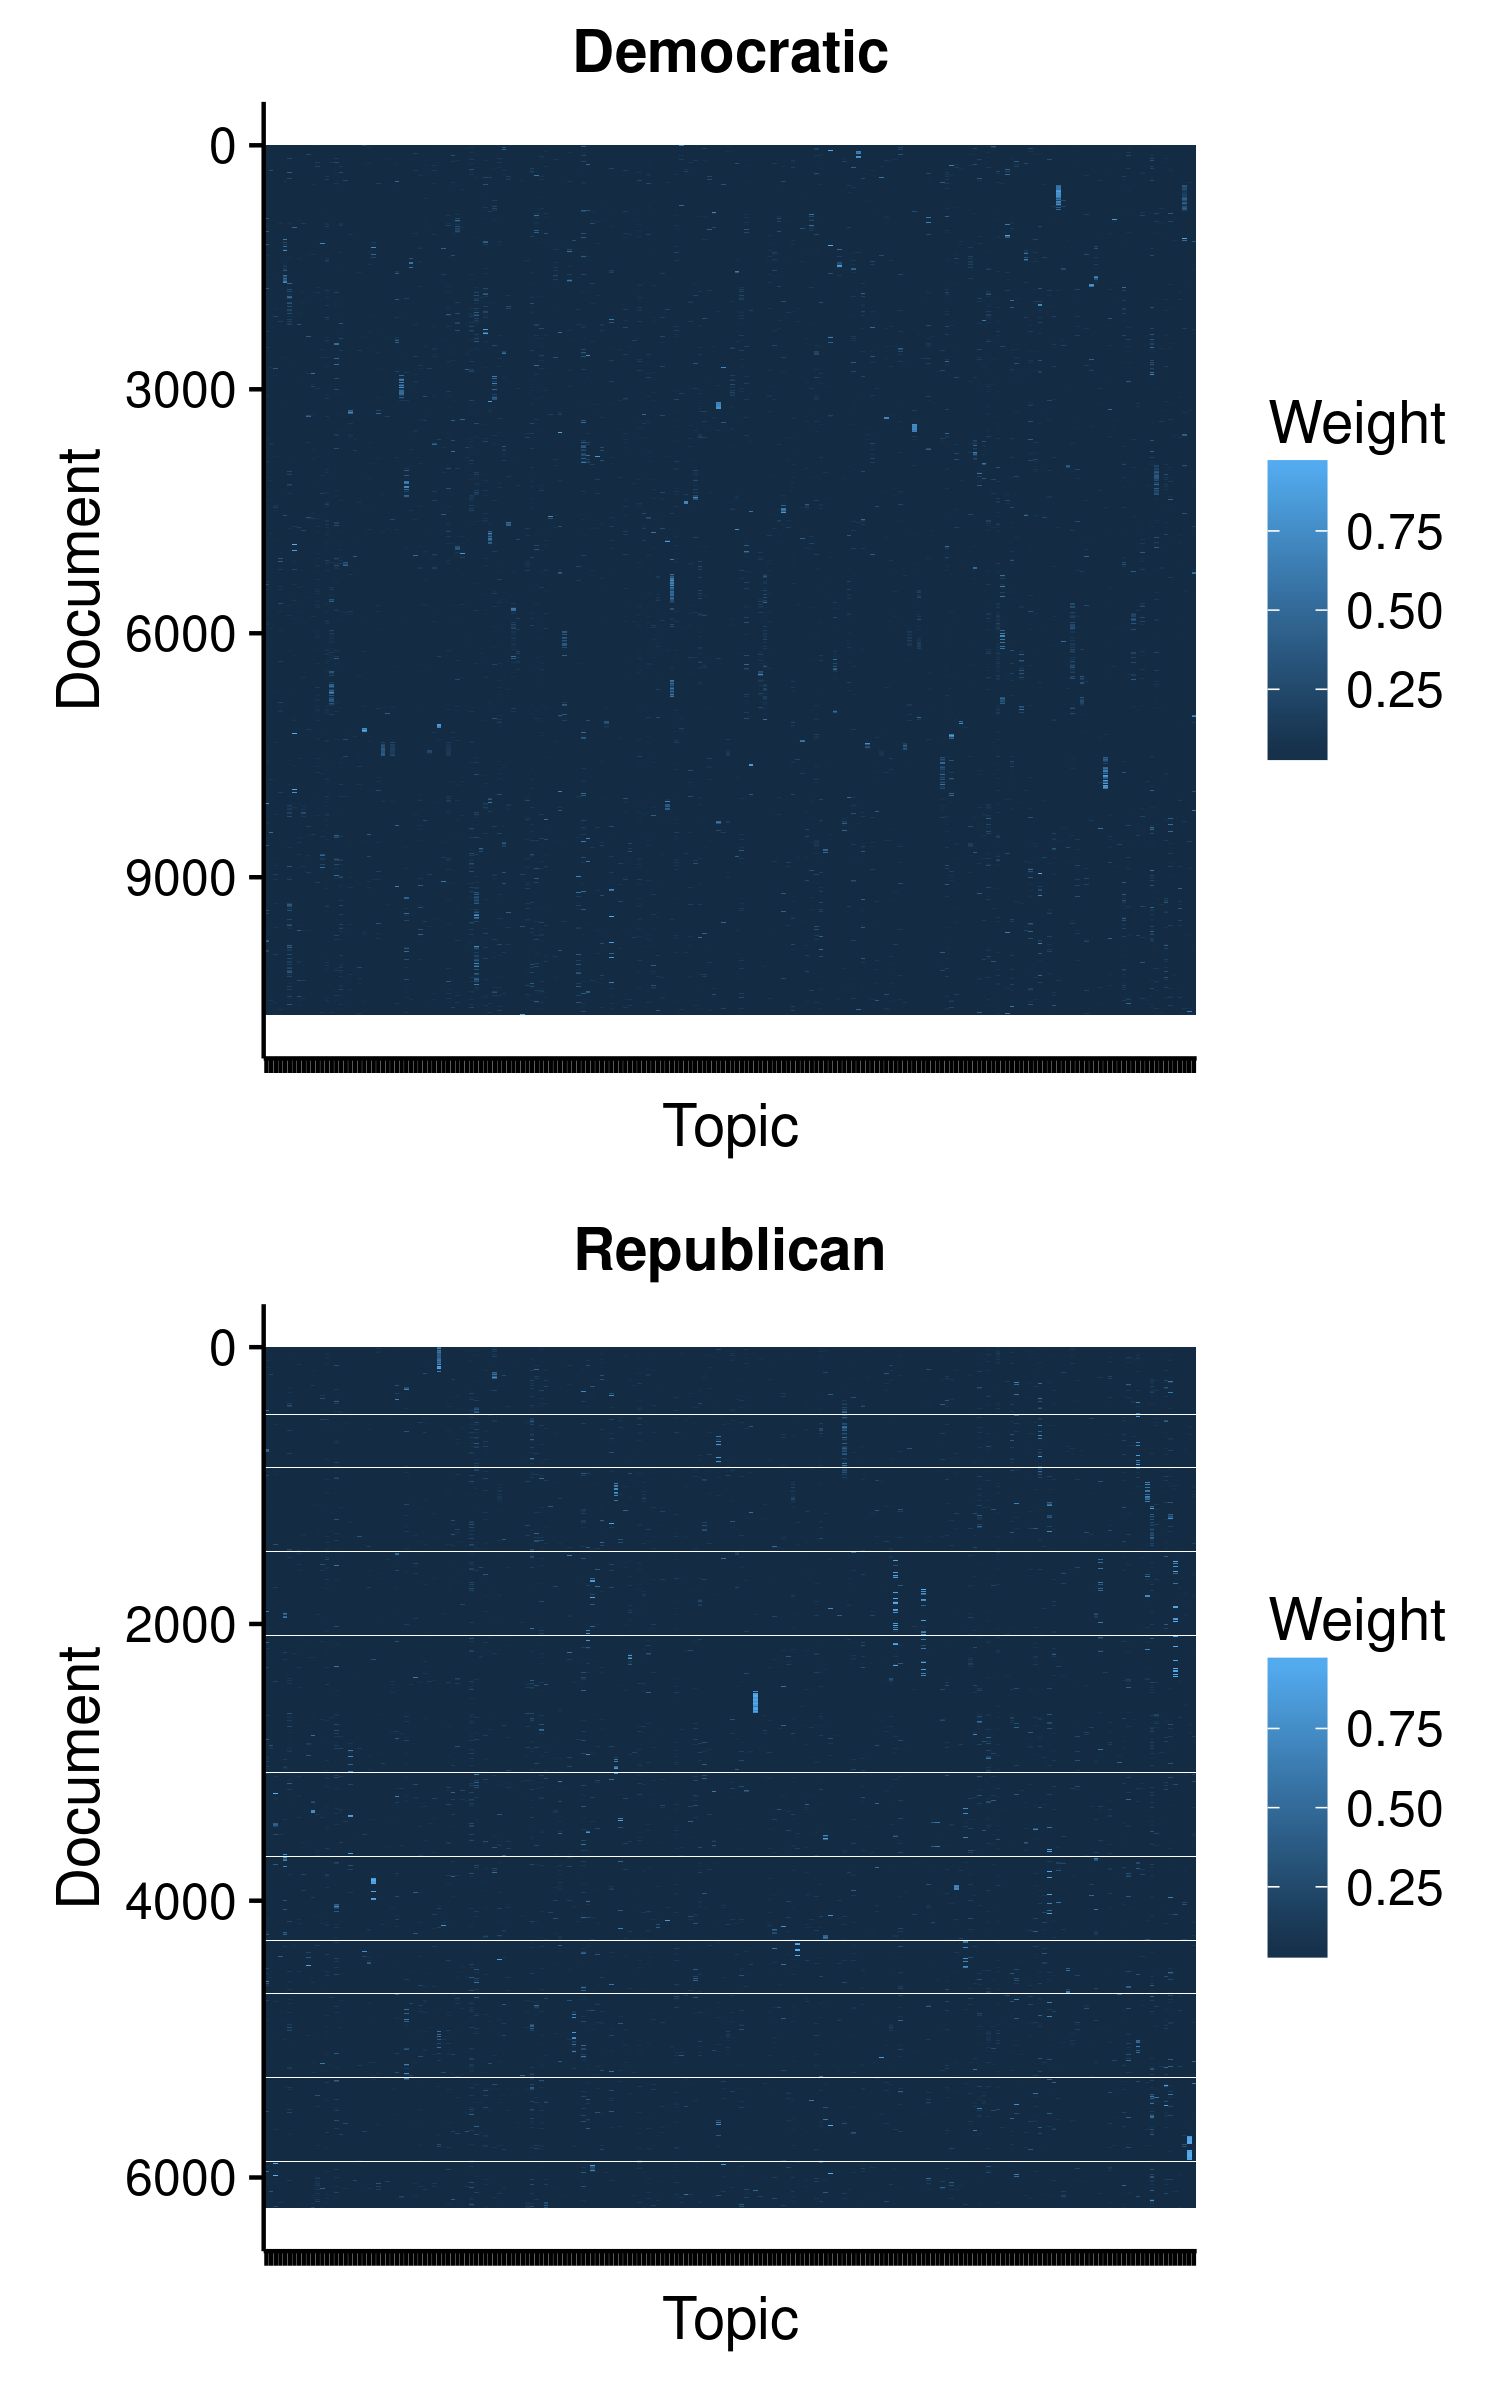
\includegraphics[width=0.8\linewidth]{figures/heatmaps_weights_IN.png}
%\end{figure}



%US map
\begin{figure}[htp]
    \centering % Using \begin{figure*} makes the figure take up the entire width of the page
    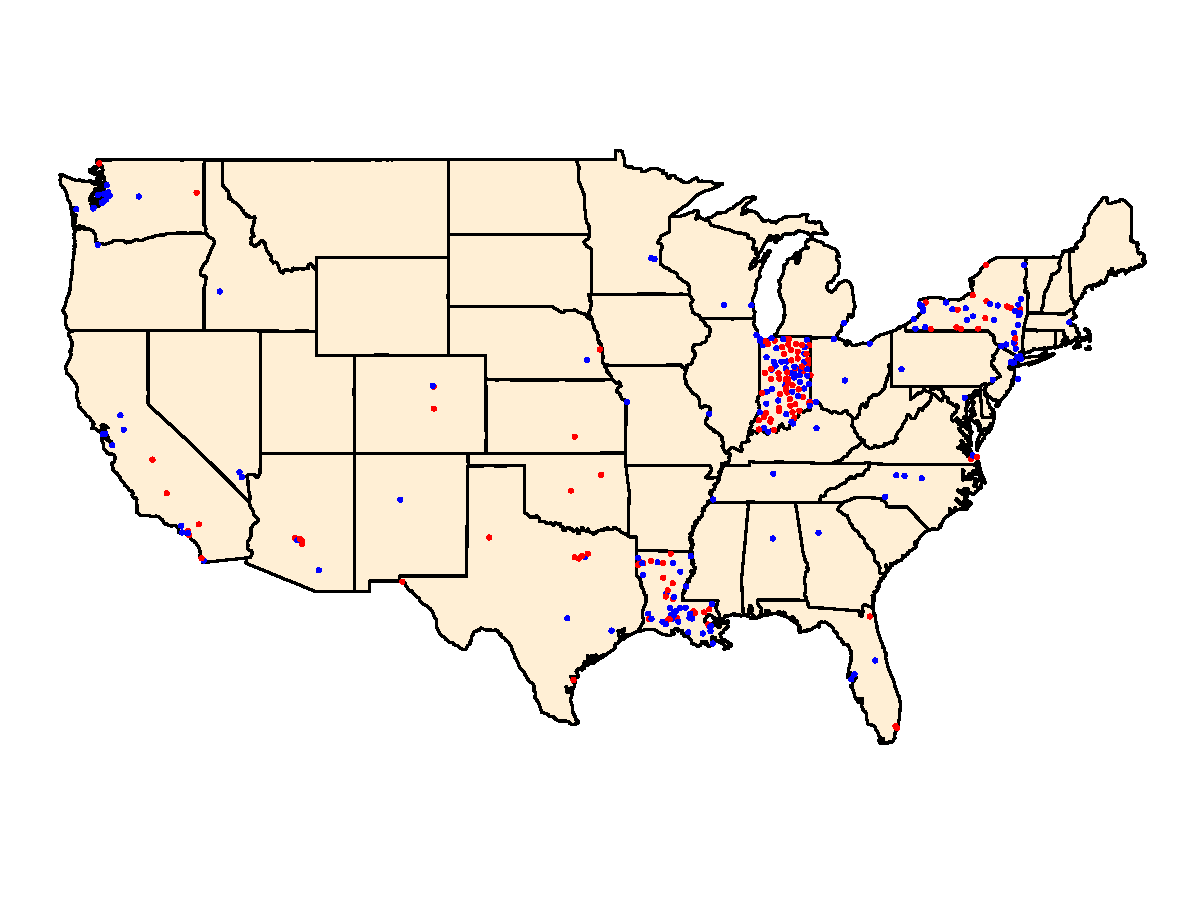
\includegraphics[width=\linewidth]{figures/us_map.pdf} \vspace{-2cm}
        \caption{Map of the cities in the corpus in the contiguous U.S. The corpus also includes Alaska. In the analysis, only cities in California, Indiana, Louisiana, New York, Texas and Washington are used. The colors represent the partisanship of the mayor (blue corresponding to Democrats and red to Republicans).}
    \label{us_map}
\end{figure}

%stm results
%\begin{figure}[htp]
%    \centering % Using \begin{figure*} makes the figure take up the entire width of the page
%    \caption{Results from a structural topic model, displayed as the p-values for each variable for each topic. This would normally be somewhat nonsensical, but here it illustrates why the model does not work.}
%    \label{stm_results}
%%    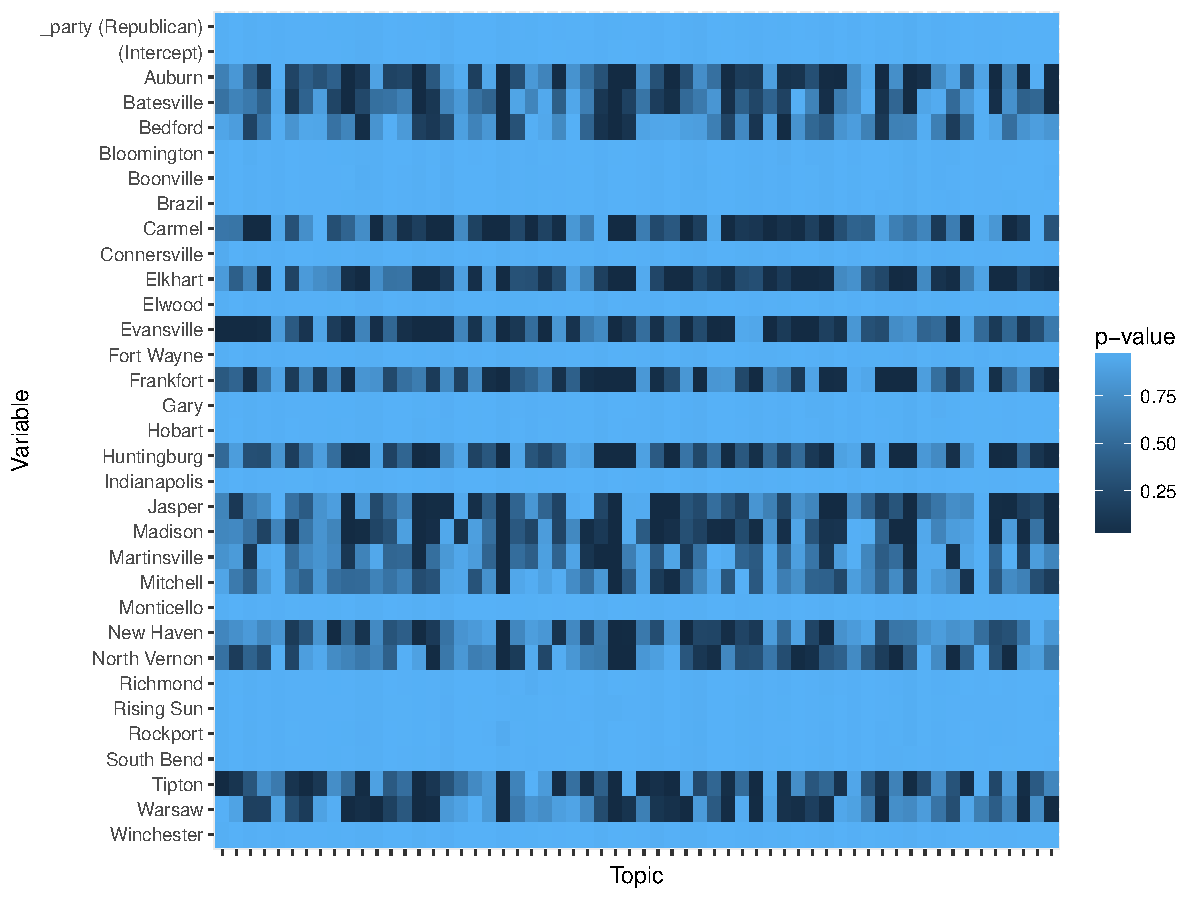
\includegraphics[width=1.1\linewidth]{figures/stm_results.pdf}
%\end{figure}



%Partisan top words - topic model Indiana
%% latex table generated in R 3.4.1 by xtable 1.8-2 package
% Fri Oct 20 13:14:52 2017
\begin{table}[ht]
\centering
\begingroup\fontsize{9pt}{10pt}\selectfont
\begin{tabular}{lrlr}
  \hline
Word (D) & Instances (D) & Word (R) & Instances (R) \\ 
  \hline
city & 42493 & will & 53761 \\ 
  said & 40480 & city & 36210 \\ 
  county & 39209 & street & 21207 \\ 
  proposal & 29019 & board & 19496 \\ 
  public & 27070 & water & 18637 \\ 
  council & 23492 & plan & 18241 \\ 
  shall & 23162 & public & 14327 \\ 
  department & 22926 & use & 13233 \\ 
  services & 22703 & information & 13062 \\ 
  fund & 21661 & development & 12916 \\ 
  will & 20697 & department & 11554 \\ 
  new & 19000 & area & 11270 \\ 
  stated & 18794 & shall & 11247 \\ 
  project & 18538 & fire & 10861 \\ 
  property & 18378 & can & 10748 \\ 
  budget & 16631 & must & 10633 \\ 
  community & 16236 & park & 10493 \\ 
  asked & 16231 & building & 10356 \\ 
  tax & 14549 & motion & 10168 \\ 
  board & 14363 & ordinance & 9625 \\ 
  state & 13964 & request & 9512 \\ 
  office & 13818 & council & 9098 \\ 
  program & 13536 & community & 9072 \\ 
  year & 13376 & meeting & 8990 \\ 
  service & 13312 & ave & 8555 \\ 
  provide & 13138 & service & 8040 \\ 
  one & 13066 & construction & 7999 \\ 
  section & 12669 & one & 7885 \\ 
  work & 11986 & property & 7741 \\ 
  information & 11886 & also & 7492 \\ 
  development & 11854 & per & 7442 \\ 
  committee & 11802 & required & 7407 \\ 
  district & 11584 & home & 7334 \\ 
  time & 11466 & center & 7316 \\ 
  total & 10965 & made & 7301 \\ 
  general & 10731 & site & 7279 \\ 
  parks & 10704 & business & 7222 \\ 
  system & 10668 & time & 7157 \\ 
  digest & 10481 & services & 7140 \\ 
  police & 10474 & housing & 7111 \\ 
  management & 10433 & new & 7006 \\ 
  park & 10356 & within & 6910 \\ 
  also & 10112 & date & 6818 \\ 
  division & 9964 & year & 6768 \\ 
  street & 9853 & following & 6754 \\ 
  resolution & 9768 & road & 6629 \\ 
  contract & 9763 & member & 6450 \\ 
  ordinance & 9456 & inc & 6367 \\ 
  safety & 9362 & number & 6360 \\ 
  code & 9342 & day & 6254 \\ 
   \hline
\end{tabular}
\endgroup
\caption{Top 50 Democratic and Republican words (Indiana), according to LDA. 
             Topic ownership is determined by the ratio of Democratic to Republican tokens in 
             it (both weighted by the total number of tokens per party). The instances of each 
             token type are then summed across all topics owned by the party.} 
\label{tabLDAIN}
\end{table}

 %\ref{tabFightinIN}

%Partisan top words - topic model Louisiana
%% latex table generated in R 3.4.1 by xtable 1.8-2 package
% Fri Oct 20 12:46:14 2017
\begin{table}[ht]
\centering
\begingroup\fontsize{9pt}{10pt}\selectfont
\begin{tabular}{lrlr}
  \hline
Word (D) & Instances (D) & Word (R) & Instances (R) \\ 
  \hline
city & 19306 & city & 9930 \\ 
  stream & 13397 & ordinance & 4413 \\ 
  new & 13001 & information & 3756 \\ 
  obj & 10440 & council & 3422 \\ 
  otherwise & 8271 & said & 3301 \\ 
  street & 7990 & plan & 3194 \\ 
  provide & 7647 & department & 2991 \\ 
  district & 7449 & state & 2598 \\ 
  property & 7031 & public & 2594 \\ 
  public & 6864 & meeting & 2392 \\ 
  shall & 6750 & mayor & 2258 \\ 
  respect & 6698 & one & 2166 \\ 
  water & 6085 & application & 2105 \\ 
  thereto & 5686 & development & 2017 \\ 
  development & 5124 & parish & 1809 \\ 
  use & 5086 & can & 1807 \\ 
  ordinance & 4963 & new & 1807 \\ 
  business & 4763 & water & 1780 \\ 
  department & 4757 & program & 1691 \\ 
  community & 4705 & project & 1674 \\ 
  authorizing & 4440 & time & 1648 \\ 
  located & 4315 & code & 1641 \\ 
  mayor & 4266 & year & 1560 \\ 
  length & 4215 & date & 1556 \\ 
  project & 3918 & number & 1548 \\ 
  section & 3863 & name & 1516 \\ 
  service & 3831 & street & 1504 \\ 
  councilman & 3824 & motion & 1500 \\ 
  services & 3782 & day & 1483 \\ 
  zoning & 3771 & park & 1471 \\ 
  parish & 3731 & home & 1469 \\ 
  providing & 3641 & address & 1415 \\ 
  one & 3636 & office & 1408 \\ 
  system & 3617 & amount & 1392 \\ 
  building & 3607 & ave & 1384 \\ 
  can & 3557 & budget & 1382 \\ 
  code & 3532 & please & 1375 \\ 
  office & 3305 & community & 1334 \\ 
  drive & 3223 & area & 1326 \\ 
  work & 3171 & contact & 1319 \\ 
  permit & 3165 & emergency & 1308 \\ 
  following & 3153 & summary & 1282 \\ 
  within & 3123 & also & 1271 \\ 
  must & 3088 & make & 1265 \\ 
  plan & 3064 & two & 1224 \\ 
  neighborhood & 3048 & work & 1213 \\ 
  construction & 3016 & fire & 1184 \\ 
  chapter & 2973 & bid & 1134 \\ 
  ordinances & 2885 & planning & 1124 \\ 
  fire & 2878 & people & 1108 \\ 
   \hline
\end{tabular}
\endgroup
\caption{Top 50 Democratic and Republican words (Louisiana), according to LDA. 
             Topic ownership is determined by the ratio of Democratic to Republican tokens in 
             it (both weighted by the total number of tokens per party). The instances of each 
             token type are then summed across all topics owned by the party.} 
\label{tabLDALA}
\end{table}

 %tabLDALA

%Partisan top words - stm Indiana
%% latex table generated in R 3.4.2 by xtable 1.8-2 package
% Tue Nov  7 21:46:14 2017
\begin{table}[ht]
\centering
\caption{Top 50 Democratic and Republican words (Indiana), according to STM. 
             The words are the top words for the most Democratic/Republican topic, determined
             by the size (and significance) of the coefficient of the party covariate.} 
\label{tabSTMIN}
\begingroup\footnotesize
\begin{tabular}{ccr|ccr}
  \toprule 
 \multicolumn{3}{c}{\textbf{Democratic}} & \multicolumn{3}{c}{\textbf{Republican}} \\
 \cmidrule(l){1-3} \cmidrule(l){4-6}
  Topic & Coefficient & Word & Topic & Coefficient & Word \\
 \midrule 
   59 & -0.026 & fort &   28 & 0.024 & motion \\ 
    59 & -0.026 & citi &   28 & 0.024 & second \\ 
    59 & -0.026 & ordin &   28 & 0.024 & made \\ 
    59 & -0.026 & approv &   28 & 0.024 & approv \\ 
    59 & -0.026 & purchas &   28 & 0.024 & mayor \\ 
    59 & -0.026 & depart &   28 & 0.024 & present \\ 
    59 & -0.026 & properti &   28 & 0.024 & state \\ 
    59 & -0.026 & will &   28 & 0.024 & will \\ 
    59 & -0.026 & resolut &   28 & 0.024 & citi \\ 
    59 & -0.026 & contract &   28 & 0.024 & council \\ 
   \cmidrule(l){1-3} \cmidrule(l){4-6}
  50 & -0.019 & propos &   11 & 0.019 & plan \\ 
    50 & -0.019 & author &   11 & 0.019 & zone \\ 
    50 & -0.019 & district &   11 & 0.019 & applic \\ 
    50 & -0.019 & street &   11 & 0.019 & properti \\ 
    50 & -0.019 & public &   11 & 0.019 & approv \\ 
    50 & -0.019 & control &   11 & 0.019 & sign \\ 
    50 & -0.019 & amend &   11 & 0.019 & site \\ 
    50 & -0.019 & intersect &   11 & 0.019 & locat \\ 
    50 & -0.019 & counti &   11 & 0.019 & commiss \\ 
    50 & -0.019 & committe &   11 & 0.019 & file \\ 
   \cmidrule(l){1-3} \cmidrule(l){4-6}
  42 & -0.018 & said &    2 & 0.019 & inc \\ 
    42 & -0.018 & ask &    2 & 0.019 & electr \\ 
    42 & -0.018 & state &    2 & 0.019 & build \\ 
    42 & -0.018 & will &    2 & 0.019 & construct \\ 
    42 & -0.018 & chair &    2 & 0.019 & home \\ 
    42 & -0.018 & propos &    2 & 0.019 & street \\ 
    42 & -0.018 & year &    2 & 0.019 & meridian \\ 
    42 & -0.018 & move &    2 & 0.019 & servic \\ 
    42 & -0.018 & need &    2 & 0.019 & west \\ 
    42 & -0.018 & council &    2 & 0.019 & main \\ 
   \cmidrule(l){1-3} \cmidrule(l){4-6}
  16 & -0.018 & prosecutor &   27 & 0.016 & request \\ 
    16 & -0.018 & charg &   27 & 0.016 & board \\ 
    16 & -0.018 & feloni &   27 & 0.016 & member \\ 
    16 & -0.018 & counti &   27 & 0.016 & servic \\ 
    16 & -0.018 & case &   27 & 0.016 & street \\ 
    16 & -0.018 & crime &   27 & 0.016 & approv \\ 
    16 & -0.018 & crimin &   27 & 0.016 & purchas \\ 
    16 & -0.018 & offic &   27 & 0.016 & citi \\ 
    16 & -0.018 & victim &   27 & 0.016 & move \\ 
    16 & -0.018 & sentenc &   27 & 0.016 & good \\ 
   \cmidrule(l){1-3} \cmidrule(l){4-6}
  13 & -0.018 & digest &   35 & 0.016 & council \\ 
    13 & -0.018 & introduc &   35 & 0.016 & citi \\ 
    13 & -0.018 & author &   35 & 0.016 & ordin \\ 
    13 & -0.018 & counti &   35 & 0.016 & common \\ 
    13 & -0.018 & appoint &   35 & 0.016 & councilor \\ 
    13 & -0.018 & board &   35 & 0.016 & amend \\ 
    13 & -0.018 & approv &   35 & 0.016 & resolut \\ 
    13 & -0.018 & district &   35 & 0.016 & adopt \\ 
    13 & -0.018 & fund &   35 & 0.016 & wherea \\ 
    13 & -0.018 & street &   35 & 0.016 & approv \\ 
   \bottomrule 
\end{tabular}
\endgroup
\end{table}

 %\ref{tabSTMLA}

%Partisan top words - stm Louisiana
%% latex table generated in R 3.4.2 by xtable 1.8-2 package
% Sun Oct 29 16:12:17 2017
\begin{table}[ht]
\centering
\begingroup\fontsize{9pt}{10pt}\selectfont
\begin{tabular}{rrlrrl}
  \hline
demTopic & demTopicCoeff & Democratic & repTopic & repTopicCoeff & Republican \\ 
  \hline
   1 & -0.171 & stream &   49 & 0.095 & event \\ 
     1 & -0.171 & obj &   49 & 0.095 & music \\ 
     1 & -0.171 & interpol &   49 & 0.095 & church \\ 
     1 & -0.171 & baa &   49 & 0.095 & inform \\ 
     1 & -0.171 & matrix &   49 & 0.095 & show \\ 
     1 & -0.171 & metadata &   49 & 0.095 & park \\ 
     1 & -0.171 & hum &   49 & 0.095 & market \\ 
     1 & -0.171 & gym &   49 & 0.095 & visit \\ 
     1 & -0.171 & rid &   49 & 0.095 & year \\ 
     1 & -0.171 & yep &   49 & 0.095 & featur \\ 
    15 & -0.045 & length &   13 & 0.093 & said \\ 
    15 & -0.045 & root &   13 & 0.093 & work \\ 
    15 & -0.045 & predictor &   13 & 0.093 & citi \\ 
    15 & -0.045 & eye &   13 & 0.093 & depart \\ 
    15 & -0.045 & word &   13 & 0.093 & airport \\ 
    15 & -0.045 & acrobat &   13 & 0.093 & code \\ 
    15 & -0.045 & adob &   13 & 0.093 & offici \\ 
    15 & -0.045 & ash &   13 & 0.093 & resid \\ 
    15 & -0.045 & rang &   13 & 0.093 & mayor \\ 
    15 & -0.045 & vet &   13 & 0.093 & continu \\ 
    57 & -0.044 & otherwis &   56 & 0.064 & ordin \\ 
    57 & -0.044 & provid &   56 & 0.064 & summari \\ 
    57 & -0.044 & respect &   56 & 0.064 & amount \\ 
    57 & -0.044 & thereto &   56 & 0.064 & citi \\ 
    57 & -0.044 & citi &   56 & 0.064 & bid \\ 
    57 & -0.044 & author &   56 & 0.064 & depart \\ 
    57 & -0.044 & ordin &   56 & 0.064 & motion \\ 
    57 & -0.044 & amend &   56 & 0.064 & approv \\ 
    57 & -0.044 & district &   56 & 0.064 & public \\ 
    57 & -0.044 & locat &   56 & 0.064 & contract \\ 
    41 & -0.017 & pdf &   12 & 0.049 & flood \\ 
    41 & -0.017 & content &   12 & 0.049 & emerg \\ 
    41 & -0.017 & type &   12 & 0.049 & storm \\ 
    41 & -0.017 & width &   12 & 0.049 & disast \\ 
    41 & -0.017 & text &   12 & 0.049 & weather \\ 
    41 & -0.017 & resourc &   12 & 0.049 & hurrican \\ 
    41 & -0.017 & parent &   12 & 0.049 & can \\ 
    41 & -0.017 & filter &   12 & 0.049 & area \\ 
    41 & -0.017 & font &   12 & 0.049 & busi \\ 
    41 & -0.017 & page &   12 & 0.049 & inform \\ 
     5 & -0.017 & polic &    3 & 0.022 & councilman \\ 
     5 & -0.017 & crime &    3 & 0.022 & want \\ 
     5 & -0.017 & offic &    3 & 0.022 & said \\ 
     5 & -0.017 & investig &    3 & 0.022 & just \\ 
     5 & -0.017 & arrest &    3 & 0.022 & know \\ 
     5 & -0.017 & suspect &    3 & 0.022 & get \\ 
     5 & -0.017 & victim &    3 & 0.022 & like \\ 
     5 & -0.017 & report &    3 & 0.022 & citi \\ 
     5 & -0.017 & block &    3 & 0.022 & can \\ 
     5 & -0.017 & vehicl &    3 & 0.022 & come \\ 
   \hline
\end{tabular}
\endgroup
\caption{Top 50 Democratic and Republican words (Louisiana), according to STM. 
             The words are the top words for the most Democratic/Republican topic, determined
             by the size (and significance) of the coefficient of the party covariate.} 
\label{tabSTMLA}
\end{table}

 %\ref{tabSTMLA}


%Some basic descriptive statistics of documents by party
%% latex table generated in R 3.4.1 by xtable 1.8-2 package
% Fri Oct 20 13:41:38 2017
\begin{table}[ht]
\centering
\begin{tabular}{rrr}
  \hline
 & Democratic & Republican \\ 
  \hline
Cities & 15 & 17 \\ 
  Documents & 10257 & 5859 \\ 
  Tokens & 6101752 & 2310072 \\ 
  Token assignments & 6006202 & 2259362 \\ 
  Topics & 103 & 97 \\ 
   \hline
\end{tabular}
\caption{Descriptive statistics for Indiana. ``Tokens'' describes the number
             of words in each party's documents, ``token assignments'' the tokens assigned
             to each party in the topic model depending on the ratio of Democratic to Republican 
             tokens in it (both weighted by the total number of tokens per party).} 
\label{tabDescriptiveIN}
\end{table}



%Some basic descriptive statistics of documents by party
%% latex table generated in R 3.4.1 by xtable 1.8-2 package
% Fri Oct 20 13:53:50 2017
\begin{table}[ht]
\centering
\begin{tabular}{rrr}
  \hline
 & Democratic & Republican \\ 
  \hline
Cities & 11 & 7 \\ 
  Documents & 6287 & 1327 \\ 
  Tokens & 1955198 & 322915 \\ 
  Token assignments & 1789373 & 314628 \\ 
  Topics & 143 & 57 \\ 
   \hline
\end{tabular}
\caption{Descriptive statistics for Louisiana. ``Tokens'' describes the number
             of words in each party's documents, ``token assignments'' the tokens assigned
             to each party in the topic model depending on the ratio of Democratic to Republican 
             tokens in it (both weighted by the total number of tokens per party).} 
\label{tabDescriptiveLA}
\end{table}



%fightin words results
%\begin{figure}[htp]
%    \centering % Using \begin{figure*} makes the figure take up the entire width of the page
%    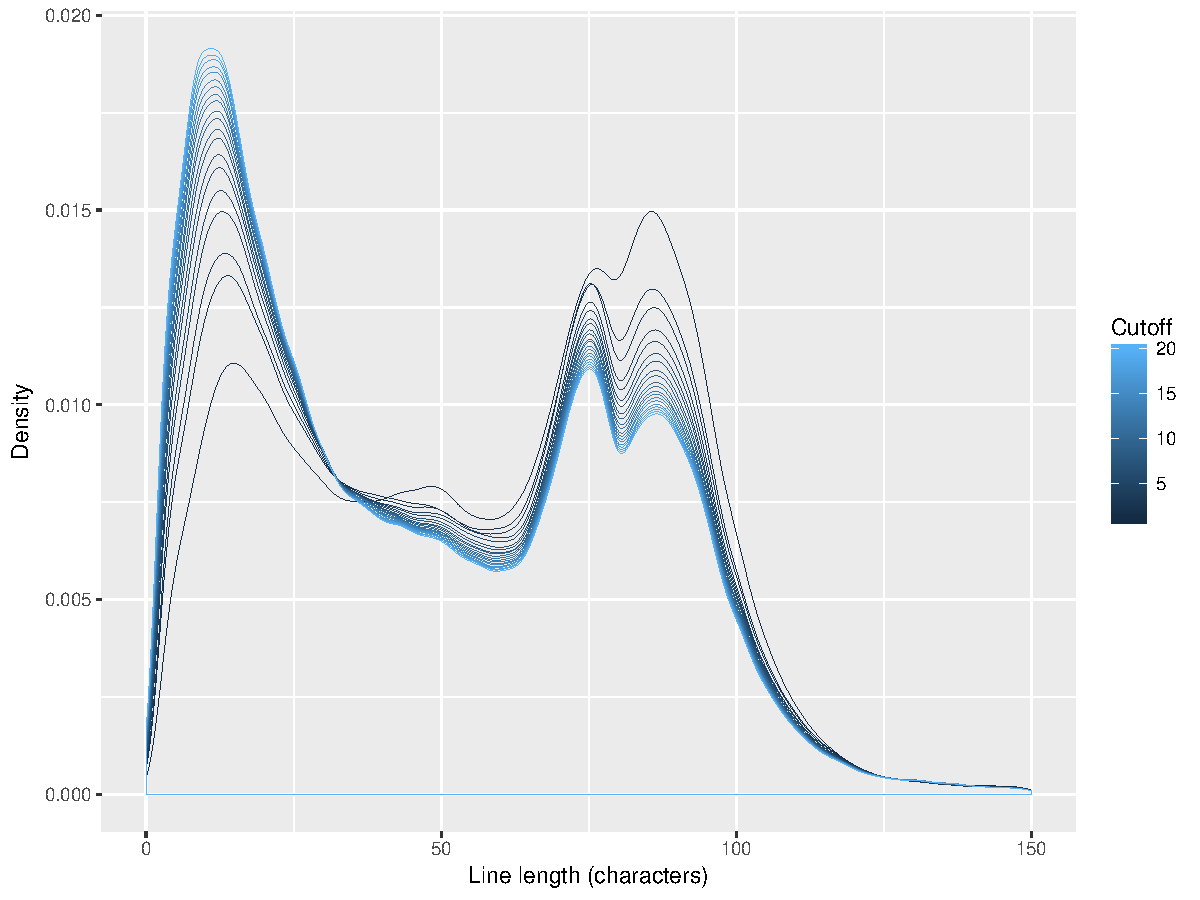
\includegraphics[width=\linewidth]{figures/linesCutoffIN.pdf}
%        \caption{Total number of lines retained at a given threshold for removing duplicated lines. For example, at x = 10, all lines occurring more than 10 times within a city's documents are removed.}
%    \label{linesCutoff}
%\end{figure}


%\section{Ground truth test}
%In the realm of public administration, the notion that the partisan leaning of mayors might have an effect on how they run their cities is still frowned upon to some extent. Perceived more as managers than politicians, they have been portrayed as the last bastion of non-partisanship in America, and in many cases, also style themselves that way \citep{Dovere2018}. However, the aspirations some mayors have shown towards higher offices - in some cases, even the presidency - reveal that they are not quite as above the fray as some may believe them to be. One of the most vicious and blatantly partisan cleavages in current U.S. politics - the debate surrounding sanctuary cities - has seen mayors in a central role. Research into local politics has shown that partisan elections consistently have greater turnout \citep{Schaffner2001}. When voters are denied this cue, they make use of other, and considerably more irrational heuristics, such as name, gender, or occupation of the contenders. Consequently, it only makes sense for any office-seeking politician to emphasize their partisanship. Finally, decades of research in political psychology have consistently shown that no matter how hard we try, humans are simply incapable of escaping our partisan biases, a finding that is especially pronounced among elites \citep{Hatemi2011}.
%
%In an effort to underline this fact and remove any doubt about the fact that the partisanship of mayors colors their decision-making, we conduct a ground truth test between our main corpus - the websites of cities - and a second, decidedly more partisan set of texts: the campaign websites of these mayors. As noted above, partisanship has been shown to be a powerful driving force even in local politics, and mayors are incentivized to exploit it. Consequently, they are very likely to emphasize conservative/liberal values on this platform. If there is a greater correlation in word use between the cities managed by a party and the campaign websites of its mayors than with those of the other party, evidence for the partisanship of city websites can be established.
%
%Using the same methods as described for our main corpus, we have gathered these sites and then concatenated all of the documents belonging to mayors of the two parties into one ground truth document each. We do the same for the city documents, and then compare the four document collections using cosine similarity. This measure is the cosine between the angle of two vectors, in this case, the frequencies of all words in the two vocabularies. Compared to a simple Euclidean distance, this has the advantage of accounting for the fact that the two corpora being compared are not necessarily of the same length. The cosine measure between two documents ranges between 0 and 1, 0 signifying absolutely no correlation, and 1 perfect overlap. Figure \ref{groundtruth} shows the result of this test. The expectation is for a greater similarity between Republican cities and the Republican ground truth than Republican cities and Democratic ground truth - and vice versa. At present, however, this does not appear to be the case, presumably because the Republican ground truth consists of 8 documents, and the Democratic one of 290.

%ground truth test
%\begin{figure}[htp]
%    \centering % Using \begin{figure*} makes the figure take up the entire width of the page
%    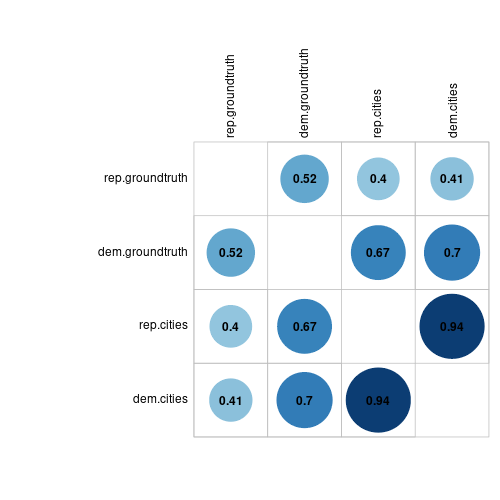
\includegraphics[width=\linewidth]{figures/groundtruth_corrplot.png}
%    \caption{Ground truth test. The values are cosine similarities between a pair of document collections.}
%    \label{groundtruth}
%\end{figure}
%
%%ground truth test
%\begin{figure}[htp]
%    \centering % Using \begin{figure*} makes the figure take up the entire width of the page
%    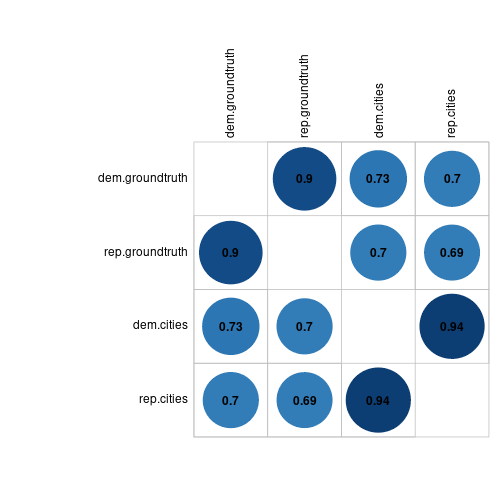
\includegraphics[width=\linewidth]{figures/groundtruth_bs_bigcities_corrplot.png}
%    \caption{Ground truth test. The values are cosine similarities between a pair of document collections (top 100 mayors vs. IN and LA).}
%    \label{groundtruth}
%\end{figure}

%Ground truth test between top100 mayors and IN + LA; with bootstrapped confidence bounds
% label: groundtruth_bootstrapped
%% latex table generated in R 3.4.3 by xtable 1.8-2 package
% Tue Feb 13 10:36:40 2018
\begin{table}[ht]
\centering
\begin{tabular}{rllll}
  \hline
 & dem.groundtruth & rep.groundtruth & dem.cities & rep.cities \\ 
  \hline
dem.groundtruth & 1, 1 & 0.807, 0.896 & 0.714, 0.729 & 0.68, 0.698 \\ 
  rep.groundtruth & 0.807, 0.896 & 1, 1 & 0.647, 0.697 & 0.641, 0.693 \\ 
  dem.cities & 0.714, 0.729 & 0.647, 0.697 & 1, 1 & 0.937, 0.944 \\ 
  rep.cities & 0.68, 0.698 & 0.641, 0.693 & 0.937, 0.944 & 1, 1 \\ 
   \hline
\end{tabular}
\caption{Ground truth test, comparing campaign websites of mayors of the 100 largest cities in the US and cities in Indiana and Louisiana. The values are bootstrapped confidence bounds for cosine similarities between concatenated document collections.} 
\label{groundtruth_bootstrapped}
\end{table}




%% latex table generated in R 3.4.4 by xtable 1.8-2 package
% Mon Apr 23 14:12:56 2018
\begin{table}[ht]
\centering
\begingroup\scriptsize
\begin{tabular}{lllllll}
  \hline
1 & 2 & 3 & 4 & 5 & 6 & 7 \\ 
  \hline
\cellcolor{red!10}yon & \cellcolor{red!10}borough & \cellcolor{red!10}port & \cellcolor{red!10}waterfront & \cellcolor{red!10}queens & \cellcolor{red!10}boroughs & \cellcolor{red!10}island \\ 
  \cellcolor{blue!10}noise & \cellcolor{blue!10}impacts & \cellcolor{blue!10}mitigation & \cellcolor{blue!10}vibration & \cellcolor{blue!10}ambient & \cellcolor{blue!10}adverse & \cellcolor{blue!10}thresholds \\ 
  \cellcolor{red!10}tax & \cellcolor{red!10}exemption & \cellcolor{red!10}taxes & \cellcolor{red!10}estate & \cellcolor{red!10}assessed & \cellcolor{red!10}real & \cellcolor{red!10}taxpayer \\ 
  \cellcolor{red!10}para & \cellcolor{red!10}personas & \cellcolor{red!10}antes & \cellcolor{red!10}persona & \cellcolor{red!10}horas & \cellcolor{red!10}junta & \cellcolor{red!10}con \\ 
  \cellcolor{blue!10}election & \cellcolor{blue!10}ethics & \cellcolor{blue!10}appointed & \cellcolor{blue!10}elections & \cellcolor{blue!10}ballot & \cellcolor{blue!10}charter & \cellcolor{blue!10}elected \\ 
  \cellcolor{red!10}wetland & \cellcolor{red!10}habitats & \cellcolor{red!10}riparian & \cellcolor{red!10}habitat & \cellcolor{red!10}wetlands & \cellcolor{red!10}tidal & \cellcolor{red!10}freshwater \\ 
  \cellcolor{blue!10}parking & \cellcolor{blue!10}bus & \cellcolor{blue!10}transit & \cellcolor{blue!10}mall & \cellcolor{blue!10}buses & \cellcolor{blue!10}campus & \cellcolor{blue!10}arena \\ 
  \cellcolor{red!30}click & \cellcolor{red!30}download & \cellcolor{red!30}online & \cellcolor{red!30}please & \cellcolor{red!30}email & \cellcolor{red!30}website & \cellcolor{red!30}visit \\ 
  \cellcolor{blue!10}draft & \cellcolor{blue!10}comments & \cellcolor{blue!10}comment & \cellcolor{blue!10}meetings & \cellcolor{blue!10}update & \cellcolor{blue!10}presentation & \cellcolor{blue!10}briefing \\ 
  \cellcolor{blue!10}ave & \cellcolor{blue!10}blvd & \cellcolor{blue!10}glen & \cellcolor{blue!10}pkwy & \cellcolor{blue!10}hwy & \cellcolor{blue!10}cove & \cellcolor{blue!10}fwy \\ 
  \cellcolor{blue!20}neighborhoods & \cellcolor{blue!20}strategy & \cellcolor{blue!20}vision & \cellcolor{blue!20}strategies & \cellcolor{blue!20}businesses & \cellcolor{blue!20}opportunities & \cellcolor{blue!20}vibrant \\ 
  \cellcolor{white}bid & \cellcolor{white}contract & \cellcolor{white}invoices & \cellcolor{white}procurement & \cellcolor{white}purchasing & \cellcolor{white}bids & \cellcolor{white}vendor \\ 
  \cellcolor{white}marijuana & \cellcolor{white}cannabis & \cellcolor{white}licensee & \cellcolor{white}taxicab & \cellcolor{white}license & \cellcolor{white}mischief & \cellcolor{white}citation \\ 
  \cellcolor{blue!10}complaint & \cellcolor{blue!10}discrimination & \cellcolor{blue!10}defendants & \cellcolor{blue!10}bankruptcy & \cellcolor{blue!10}trial & \cellcolor{blue!10}harassment & \cellcolor{blue!10}defendant \\ 
  \cellcolor{red!10}rouge & \cellcolor{red!10}baton & \cellcolor{red!10}foods & \cellcolor{red!10}parish & \cellcolor{red!10}vegetables & \cellcolor{red!10}vending & \cellcolor{red!10}cooked \\ 
  \cellcolor{red!10}child & \cellcolor{red!10}violence & \cellcolor{red!10}abuse & \cellcolor{red!10}mental & \cellcolor{red!10}clients & \cellcolor{red!10}inmates & \cellcolor{red!10}homelessness \\ 
  \cellcolor{red!10}applicants & \cellcolor{red!10}landlord & \cellcolor{red!10}tenant & \cellcolor{red!10}rent & \cellcolor{red!10}exam & \cellcolor{red!10}tenants & \cellcolor{red!10}applications \\ 
  \cellcolor{red!10}think & \cellcolor{red!10}say & \cellcolor{red!10}really & \cellcolor{red!10}thing & \cellcolor{red!10}okay & \cellcolor{red!10}got & \cellcolor{red!10}maybe \\ 
  \cellcolor{blue!20}setback & \cellcolor{blue!20}fence & \cellcolor{blue!20}yard & \cellcolor{blue!20}zoned & \cellcolor{blue!20}front & \cellcolor{blue!20}height & \cellcolor{blue!20}accessory \\ 
  \cellcolor{red!10}shall & \cellcolor{red!10}subsection & \cellcolor{red!10}article & \cellcolor{red!10}provisions & \cellcolor{red!10}pursuant & \cellcolor{red!10}thereof & \cellcolor{red!10}forth \\ 
  \cellcolor{red!20}explained & \cellcolor{red!20}asked & \cellcolor{red!20}said & \cellcolor{red!20}legislator & \cellcolor{red!20}commented & \cellcolor{red!20}advised & \cellcolor{red!20}leg \\ 
  \cellcolor{blue!10}respondents & \cellcolor{blue!10}census & \cellcolor{blue!10}population & \cellcolor{blue!10}compared & \cellcolor{blue!10}average & \cellcolor{blue!10}trends & \cellcolor{blue!10}comparison \\ 
  \cellcolor{red!20}infection & \cellcolor{red!20}symptoms & \cellcolor{red!20}breastfeeding & \cellcolor{red!20}syphilis & \cellcolor{red!20}doses & \cellcolor{red!20}asthma & \cellcolor{red!20}tuberculosis \\ 
  \cellcolor{red!20}yes & \cellcolor{red!20}name & \cellcolor{red!20}signature & \cellcolor{red!20}mailing & \cellcolor{red!20}zip & \cellcolor{red!20}attach & \cellcolor{red!20}form \\ 
  \cellcolor{red!30}games & \cellcolor{red!30}tournament & \cellcolor{red!30}swim & \cellcolor{red!30}players & \cellcolor{red!30}player & \cellcolor{red!30}camp & \cellcolor{red!30}game \\ 
  \cellcolor{blue!10}goals & \cellcolor{blue!10}implementation & \cellcolor{blue!10}policies & \cellcolor{blue!10}policy & \cellcolor{blue!10}specific & \cellcolor{blue!10}implement & \cellcolor{blue!10}comprehensive \\ 
  \cellcolor{red!20}ems & \cellcolor{red!20}fires & \cellcolor{red!20}preparedness & \cellcolor{red!20}disaster & \cellcolor{red!20}evacuation & \cellcolor{red!20}fire & \cellcolor{red!20}firefighters \\ 
  \cellcolor{red!10}subcontractor & \cellcolor{red!10}subcontractors & \cellcolor{red!10}agrees & \cellcolor{red!10}proposer & \cellcolor{red!10}contractor & \cellcolor{red!10}grantee & \cellcolor{red!10}breach \\ 
  \cellcolor{blue!10}realm & \cellcolor{blue!10}massing & \cellcolor{blue!10}facades & \cellcolor{blue!10}entrances & \cellcolor{blue!10}plazas & \cellcolor{blue!10}elements & \cellcolor{blue!10}proponents \\ 
  \cellcolor{blue!10}employee & \cellcolor{blue!10}allegation & \cellcolor{blue!10}overtime & \cellcolor{blue!10}named & \cellcolor{blue!10}leave & \cellcolor{blue!10}grievance & \cellcolor{blue!10}wage \\ 
  \cellcolor{blue!10}parks & \cellcolor{blue!10}playground & \cellcolor{blue!10}beach & \cellcolor{blue!10}park & \cellcolor{blue!10}picnic & \cellcolor{blue!10}marina & \cellcolor{blue!10}trails \\ 
  \cellcolor{blue!10}lanes & \cellcolor{blue!10}bicycle & \cellcolor{blue!10}bike & \cellcolor{blue!10}intersections & \cellcolor{blue!10}bicyclists & \cellcolor{blue!10}roadway & \cellcolor{blue!10}pedestrians \\ 
  \cellcolor{blue!20}absent & \cellcolor{blue!20}aye & \cellcolor{blue!20}khan & \cellcolor{blue!20}voting & \cellcolor{blue!20}berry & \cellcolor{blue!20}nays & \cellcolor{blue!20}tagged \\ 
  \cellcolor{blue!20}budget & \cellcolor{blue!20}revenue & \cellcolor{blue!20}million & \cellcolor{blue!20}revenues & \cellcolor{blue!20}budgeted & \cellcolor{blue!20}fund & \cellcolor{blue!20}expenditures \\ 
  \cellcolor{blue!10}whereas & \cellcolor{blue!10}resolution & \cellcolor{blue!10}amending & \cellcolor{blue!10}resolved & \cellcolor{blue!10}hereby & \cellcolor{blue!10}authorizes & \cellcolor{blue!10}digest \\ 
  \cellcolor{blue!10}assets & \cellcolor{blue!10}statements & \cellcolor{blue!10}governmental & \cellcolor{blue!10}accounting & \cellcolor{blue!10}liabilities & \cellcolor{blue!10}net & \cellcolor{blue!10}financial \\ 
  \cellcolor{red!30}honored & \cellcolor{red!30}joined & \cellcolor{red!30}proud & \cellcolor{red!30}fort & \cellcolor{red!30}announces & \cellcolor{red!30}won & \cellcolor{red!30}worth \\ 
  \cellcolor{white}analyst & \cellcolor{white}technician & \cellcolor{white}specialist & \cellcolor{white}performs & \cellcolor{white}prepares & \cellcolor{white}coordinates & \cellcolor{white}assists \\ 
  \cellcolor{white}server & \cellcolor{white}wireless & \cellcolor{white}software & \cellcolor{white}aircraft & \cellcolor{white}servers & \cellcolor{white}airport & \cellcolor{white}technology \\ 
  \cellcolor{blue!10}improvements & \cellcolor{blue!10}project & \cellcolor{blue!10}projects & \cellcolor{blue!10}phase & \cellcolor{blue!10}replacement & \cellcolor{blue!10}reconstruction & \cellcolor{blue!10}upgrades \\ 
  \cellcolor{red!10}recycling & \cellcolor{red!10}recycle & \cellcolor{red!10}garbage & \cellcolor{red!10}bags & \cellcolor{red!10}waste & \cellcolor{red!10}recyclable & \cellcolor{red!10}recyclables \\ 
  \cellcolor{blue!10}housing & \cellcolor{blue!10}affordable & \cellcolor{blue!10}households & \cellcolor{blue!10}affordability & \cellcolor{blue!10}income & \cellcolor{blue!10}moderate & \cellcolor{blue!10}homeless \\ 
  \cellcolor{red!20}effluent & \cellcolor{red!20}wastewater & \cellcolor{red!20}discharges & \cellcolor{red!20}contaminants & \cellcolor{red!20}sludge & \cellcolor{red!20}infiltration & \cellcolor{red!20}solids \\ 
  \cellcolor{red!10}fee & \cellcolor{red!10}permit & \cellcolor{red!10}inspection & \cellcolor{red!10}permits & \cellcolor{red!10}inspections & \cellcolor{red!10}fees & \cellcolor{red!10}occupancy \\ 
  \cellcolor{blue!10}uses & \cellcolor{blue!10}mixed & \cellcolor{blue!10}density & \cellcolor{blue!10}land & \cellcolor{blue!10}industrial & \cellcolor{blue!10}residential & \cellcolor{blue!10}commercial \\ 
  \cellcolor{red!10}energy & \cellcolor{red!10}renewable & \cellcolor{red!10}coal & \cellcolor{red!10}electricity & \cellcolor{red!10}climate & \cellcolor{red!10}solar & \cellcolor{red!10}greenhouse \\ 
  \cellcolor{blue!10}bonds & \cellcolor{blue!10}refunding & \cellcolor{blue!10}securities & \cellcolor{blue!10}bond & \cellcolor{blue!10}debt & \cellcolor{blue!10}issuer & \cellcolor{blue!10}maturity \\ 
  \cellcolor{red!20}artists & \cellcolor{red!20}artist & \cellcolor{red!20}performances & \cellcolor{red!20}music & \cellcolor{red!20}orchestra & \cellcolor{red!20}symphony & \cellcolor{red!20}arts \\ 
  \cellcolor{blue!80}arrested & \cellcolor{blue!80}suspect & \cellcolor{blue!80}homicide & \cellcolor{blue!80}suspects & \cellcolor{blue!80}shooting & \cellcolor{blue!80}sergeant & \cellcolor{blue!80}arrests \\ 
  \cellcolor{white}retiree & \cellcolor{white}actuarial & \cellcolor{white}retirement & \cellcolor{white}deductible & \cellcolor{white}retirees & \cellcolor{white}copay & \cellcolor{white}dental \\ 
  \cellcolor{red!10}ferrets & \cellcolor{red!10}dogs & \cellcolor{red!10}cats & \cellcolor{red!10}rabies & \cellcolor{red!10}pets & \cellcolor{red!10}spay & \cellcolor{red!10}stray \\ 
  \cellcolor{blue!10}audit & \cellcolor{blue!10}auditor & \cellcolor{blue!10}audits & \cellcolor{blue!10}procedures & \cellcolor{blue!10}controls & \cellcolor{blue!10}implemented & \cellcolor{blue!10}accountability \\ 
  \cellcolor{blue!10}avenue & \cellcolor{blue!10}west & \cellcolor{blue!10}east & \cellcolor{blue!10}south & \cellcolor{blue!10}north & \cellcolor{blue!10}thence & \cellcolor{blue!10}street \\ 
  \cellcolor{white}historic & \cellcolor{white}revival & \cellcolor{white}landmarks & \cellcolor{white}landmark & \cellcolor{white}craftsman & \cellcolor{white}bungalow & \cellcolor{white}style \\ 
  \cellcolor{red!10}remodel & \cellcolor{red!10}monoxide & \cellcolor{red!10}alarms & \cellcolor{red!10}roofing & \cellcolor{red!10}heater & \cellcolor{red!10}description & \cellcolor{red!10}bathroom \\ 
  \cellcolor{red!10}motion & \cellcolor{red!10}alderman & \cellcolor{red!10}seconded & \cellcolor{red!10}carried & \cellcolor{red!10}whiting & \cellcolor{red!10}unanimously & \cellcolor{red!10}ayes \\ 
  \cellcolor{white}pruning & \cellcolor{white}tree & \cellcolor{white}forestry & \cellcolor{white}trees & \cellcolor{white}mulch & \cellcolor{white}planting & \cellcolor{white}planted \\ 
  \cellcolor{red!10}fittings & \cellcolor{red!10}joints & \cellcolor{red!10}thickness & \cellcolor{red!10}pipe & \cellcolor{red!10}trench & \cellcolor{red!10}valve & \cellcolor{red!10}psi \\ 
  \cellcolor{white}students & \cellcolor{white}learning & \cellcolor{white}schools & \cellcolor{white}student & \cellcolor{white}academic & \cellcolor{white}career & \cellcolor{white}education \\ 
  \cellcolor{red!20}plat & \cellcolor{red!20}sign & \cellcolor{red!20}pud & \cellcolor{red!20}petitioner & \cellcolor{red!20}petition & \cellcolor{red!20}variance & \cellcolor{red!20}subdivision \\ 
   \hline
\end{tabular}
\endgroup
\caption{Top words from a structural topic model with 60 topics and FREX scoring. Colors depict partisanship based on coefficient size. White cells are non-significant topics. Based on data preprocessed without the classifier.} 
\end{table}

 %\ref{tabSTMtopwords}


% latex table generated in R 3.4.4 by xtable 1.8-2 package
% Fri Aug 10 15:33:35 2018
\begin{table}[ht]
\centering
\begingroup\footnotesize
\begin{tabular}{rllllllll}
  \hline
 \# & Top Word 1 & Top Word 2 & Top Word 3 & Top Word 4 & Top Word 5 & Top Word 6 & \multicolumn{2}{c}{Tokens assigned} \\ 
  \hline
   42 & \cellcolor{red!20}breastfeed & \cellcolor{red!20}vaccine & \cellcolor{red!20}infection & \cellcolor{red!20}symptom & \cellcolor{red!20}asthma & \cellcolor{red!20}mosquito & \mybar{2497} \\ 
   17 & \cellcolor{red!20}alarm & \cellcolor{red!20}disaster & \cellcolor{red!20}fire & \cellcolor{red!20}rescue & \cellcolor{red!20}preparedness & \cellcolor{red!20}evacuation & \mybar{989} \\ 
   53 & \cellcolor{red!20}drinking & \cellcolor{red!20}wastewater & \cellcolor{red!20}water & \cellcolor{red!20}pipeline & \cellcolor{red!20}pump & \cellcolor{red!20}disinfection & \mybar{461} \\ 

   49 & \cellcolor{red!10}bin & \cellcolor{red!10}recycling & \cellcolor{red!10}garbage & \cellcolor{red!10}recyclables & \cellcolor{red!10}recyclable & \cellcolor{red!10}bag & \mybar{1791} \\ 
    7 & \cellcolor{red!10}energy & \cellcolor{red!10}garland & \cellcolor{red!10}renewable & \cellcolor{red!10}solar & \cellcolor{red!10}electricity & \cellcolor{red!10}climate & \mybar{742} \\ 
   23 & \cellcolor{red!10}bid & \cellcolor{red!10}proposer & \cellcolor{red!10}bidder & \cellcolor{red!10}contractor & \cellcolor{red!10}subcontractor & \cellcolor{red!10}contract & \mybar{447} \\ 
   57 & \cellcolor{red!10}duct & \cellcolor{red!10}conduit & \cellcolor{red!10}bolt & \cellcolor{red!10}splice & \cellcolor{red!10}valve & \cellcolor{red!10}fitting & \mybar{1373} \\ 
   13 & \cellcolor{red!10}server & \cellcolor{red!10}wireless & \cellcolor{red!10}software & \cellcolor{red!10}telecommunication & \cellcolor{red!10}subscriber & \cellcolor{red!10}desktop & \mybar{1092} \\ 
    1 & \cellcolor{red!10}storm & \cellcolor{red!10}runoff & \cellcolor{red!10}infiltration & \cellcolor{red!10}discharge & \cellcolor{red!10}drainage & \cellcolor{red!10}drain & \mybar{516} \\ 
   38 & \cellcolor{red!10}youth & \cellcolor{red!10}student & \cellcolor{red!10}parent & \cellcolor{red!10}teacher & \cellcolor{red!10}immigrant & \cellcolor{red!10}literacy & \mybar{714} \\ 
   59 & \cellcolor{red!10}sampling & \cellcolor{red!10}sample & \cellcolor{red!10}analytical & \cellcolor{red!10}concentration & \cellcolor{red!10}hydrocarbon & \cellcolor{red!10}toxicity & \mybar{1241} \\ 
   45 & \cellcolor{red!10}premise & \cellcolor{red!10}licensee & \cellcolor{red!10}violation & \cellcolor{red!10}license & \cellcolor{red!10}permit & \cellcolor{red!10}inspection & \mybar{509} \\ 
   60 & \cellcolor{red!10}exhaust & \cellcolor{red!10}fugitive & \cellcolor{red!10}aircraft & \cellcolor{red!10}airport & \cellcolor{red!10}aviation & \cellcolor{red!10}diesel & \mybar{731} \\ 
   %30 & \cellcolor{white}fort & \cellcolor{white}thence & \cellcolor{white}blvd & \cellcolor{white}worth & \cellcolor{white}ave & \cellcolor{white}west & \mybar{681} \\ 
   %58 & \cellcolor{white}councilor & \cellcolor{white}auburn & \cellcolor{white}plain & \cellcolor{white}ward & \cellcolor{white}beech & \cellcolor{white}glen & \mybar{480} \\ 
   %51 & \cellcolor{white}whereas & \cellcolor{white}councilman & \cellcolor{white}alderman & \cellcolor{white}ordain & \cellcolor{white}hereby & \cellcolor{white}resolution & \mybar{420} \\ 
   %16 & \cellcolor{white}recreation & \cellcolor{white}park & \cellcolor{white}golf & \cellcolor{white}playground & \cellcolor{white}picnic & \cellcolor{white}zoo & \mybar{682} \\ 
   %36 & \cellcolor{white}retiree & \cellcolor{white}retirement & \cellcolor{white}actuarial & \cellcolor{white}deductible & \cellcolor{white}dental & \cellcolor{white}pension & \mybar{470} \\ 
   %27 & \cellcolor{white}exam & \cellcolor{white}incumbent & \cellcolor{white}supervise & \cellcolor{white}supervision & \cellcolor{white}examination & \cellcolor{white}knowledge & \mybar{687} \\ 
   %56 & \cellcolor{white}historic & \cellcolor{white}landmark & \cellcolor{white}revival & \cellcolor{white}archaeological & \cellcolor{white}century & \cellcolor{white}historian & \mybar{2587} \\ 
   %12 & \cellcolor{white}parking & \cellcolor{white}hotel & \cellcolor{white}garage & \cellcolor{white}space & \cellcolor{white}retail & \cellcolor{white}square & \mybar{321} \\ 
   %41 & \cellcolor{white}tax & \cellcolor{white}exemption & \cellcolor{white}abatement & \cellcolor{white}real & \cellcolor{white}estate & \cellcolor{white}property & \mybar{310} \\ 
    4 & \cellcolor{white}facade & \cellcolor{white}awning & \cellcolor{white}porch & \cellcolor{white}roof & \cellcolor{white}balcony & \cellcolor{white}exterior & \mybar{1108} \\ 

   15 & \cellcolor{blue!10}complainant & \cellcolor{blue!10}defendant & \cellcolor{blue!10}allegation & \cellcolor{blue!10}complaint & \cellcolor{blue!10}allege & \cellcolor{blue!10}discrimination & \mybar{1384} \\ 
 
   14 & \cellcolor{blue!10}yes & \cellcolor{blue!10}agency & \cellcolor{blue!10}federal & \cellcolor{blue!10}recipient & \cellcolor{blue!10}compliance & \cellcolor{blue!10}entity & \mybar{205} \\ 

   25 & \cellcolor{blue!10}cannabis & \cellcolor{blue!10}marijuana & \cellcolor{blue!10}senate & \cellcolor{blue!10}dispensary & \cellcolor{blue!10}ballot & \cellcolor{blue!10}cultivation & \mybar{1188} \\ 

   47 & \cellcolor{blue!10}employee & \cellcolor{blue!10}overtime & \cellcolor{blue!10}sick & \cellcolor{blue!10}wage & \cellcolor{blue!10}grievance & \cellcolor{blue!10}bargaining & \mybar{511} \\ 

   37 & \cellcolor{blue!10}audit & \cellcolor{blue!10}auditor & \cellcolor{blue!10}internal & \cellcolor{blue!10}procedure & \cellcolor{blue!10}accountability & \cellcolor{blue!10}oversight & \mybar{420} \\ 
   21 & \cellcolor{blue!10}housing & \cellcolor{blue!10}affordable & \cellcolor{blue!10}homeless & \cellcolor{blue!10}homelessness & \cellcolor{blue!10}affordability & \cellcolor{blue!10}landlord & \mybar{318} \\ 
   34 & \cellcolor{blue!10}comment & \cellcolor{blue!10}draft & \cellcolor{blue!10}feedback & \cellcolor{blue!10}stakeholder & \cellcolor{blue!10}suggest & \cellcolor{blue!10}discussion & \mybar{289} \\ 
   19 & \cellcolor{blue!10}debt & \cellcolor{blue!10}bond & \cellcolor{blue!10}governmental & \cellcolor{blue!10}obligation & \cellcolor{blue!10}financial & \cellcolor{blue!10}accounting & \mybar{251} \\ 
   40 & \cellcolor{blue!10}bicycle & \cellcolor{blue!10}bike & \cellcolor{blue!10}lane & \cellcolor{blue!10}crosswalk & \cellcolor{blue!10}pedestrian & \cellcolor{blue!10}bicyclist & \mybar{574} \\ 
   32 & \cellcolor{blue!20}budget & \cellcolor{blue!20}revenue & \cellcolor{blue!20}expenditure & \cellcolor{blue!20}appropriation & \cellcolor{blue!20}fund & \cellcolor{blue!20}million & \mybar{242} \\ 
   48 & \cellcolor{blue!20}absent & \cellcolor{blue!20}aye & \cellcolor{blue!20}khan & \cellcolor{blue!20}nay & \cellcolor{blue!20}berry & \cellcolor{blue!20}voting & \mybar{528} \\ 
   31 & \cellcolor{blue!20}chair & \cellcolor{blue!20}agenda & \cellcolor{blue!20}commission & \cellcolor{blue!20}speaker & \cellcolor{blue!20}chairperson & \cellcolor{blue!20}committee & \mybar{314} \\ 
   55 & \cellcolor{blue!80}robbery & \cellcolor{blue!80}homicide & \cellcolor{blue!80}arrest & \cellcolor{blue!80}sergeant & \cellcolor{blue!80}suspect & \cellcolor{blue!80}burglary & \mybar{1395} \\ 
   \hline
\end{tabular}
\endgroup
%\caption{Top words from a structural topic model with 60 topics and FREX scoring. Colors depict partisanship based on coefficient size. White cells are non-significant topics.} 
\label{tabSTMtopwords60}
\end{table}

 %\ref{tabSTMtopwords2}

\section{Conclusion}


We have developed a methodological pipeline for automatically gathering and preparing government websites for comparative content analysis. This methodology holds the potential to vastly scale up the data collection efforts underpinning the growing body of research that is focused on government website analysis. The methods involved in the pipeline include checking the integrity of the site addresses, extracting English language from website contents, identifying document types, and removing boilerplate language. Government website contents can, and have been, used to study questions related representation, government transparency, and public policy priorities. The methods we develop can be used to scale up projects involving website data collection by automating the process. 

In terms of pure scope, our method is superior to the existing approaches. Manual content analysis (see, for example, \cite{Druckman2009}) relies on research assistants reading and evaluating websites, and therefore might struggle to provide a complete understanding of even individual websites, which often contain thousands of pages. Scrapers conventionally used in the social sciences (see, for example, \citealt{Cryer2017}) rely on extracting text through specific HTML tags, which makes it difficult to apply to a large number of websites, because the process needs to be adjusted for each one. By contrast, the only input our pipeline requires is the URL, and the only limits are bandwidth, processing power and storage space. Consequently, our approach facilitates the kind of bulk data collection and analysis necessitated by an ever-growing web.

Through an application to the analysis of municipal websites in six different states, we show how our pipeline is capable of gathering corpora that shed light on the forms and functions of local government. We find that government website contents are associated with the partisanship of the mayor in ways that would be expected based on the parties' national priorities and past research on the effects of mayoral partisanship on city governments.

We offer several contributions that will be valuable in future research endeavors. First, the data collected in the current study can be used for comparative analysis of US city website contents. Second, the pipeline we present can be used as a set of procedures to follow in gathering large-scale datasets of textual contents from other samples of governments. For example, the pipeline we have developed could be used to build comparative datasets of state or federal bureaucratic agencies. Third, our findings regarding the effects of mayoral partisanship on city website contents advance the literature on the role of partisan leadership in local government, and reinforce the finding of \citet{gerber2011mayors} that the effects of mayoral partisanship can be best observed through the analysis of domains of government (e.g., website contents) that are not heavily constrained by state or national governments.


%% latex table generated in R 3.5.0 by xtable 1.8-2 package
% Wed Jul  4 14:14:10 2018
\begin{table}[ht]
\centering
\begin{tabular}{lrr}
  \hline
State & Democratic & Republican \\ 
  \hline
California &   9 &   6 \\ 
  Indiana &  46 &  54 \\ 
  Louisiana &  28 &  17 \\ 
  New York &  36 &  16 \\ 
  Texas &   2 &   7 \\ 
  Washington &  11 &   2 \\ 
   \hline
\end{tabular}
\caption{Descriptive statistics on the partisanship of the cities in the corpus.} 
\end{table}


%% latex table generated in R 3.4.3 by xtable 1.8-2 package
% Fri Mar  2 19:05:45 2018
\begin{table}[ht]
\centering
\begin{tabular}{lr}
  \hline
State & Cities \\ 
  \hline
Alabama &   1 \\ 
  Alaska &   1 \\ 
  Arizona &   6 \\ 
  California &  15 \\ 
  Colorado &   3 \\ 
  D.C. &   1 \\ 
  Florida &   6 \\ 
  Georgia &   1 \\ 
  Hawaii &   1 \\ 
  Idaho &   1 \\ 
  Illinois &   1 \\ 
  Indiana & 108 \\ 
  Kansas &   1 \\ 
  Kentucky &   2 \\ 
  Louisiana &  57 \\ 
  Maryland &   1 \\ 
  Massachusetts &   1 \\ 
  Michigan &   1 \\ 
  Minnesota &   2 \\ 
  Missouri &   2 \\ 
  Nebraska &   2 \\ 
  Nevada &   2 \\ 
  New Jersey &   2 \\ 
  New Mexico &   1 \\ 
  New York &  52 \\ 
  North Carolina &   4 \\ 
  Ohio &   4 \\ 
  Oklahoma &   2 \\ 
  Oregon &   1 \\ 
  Pennsylvania &   2 \\ 
  Tennessee &   2 \\ 
  Texas &  10 \\ 
  Virginia &   3 \\ 
  Washington &  13 \\ 
  Wisconsin &   2 \\ 
   \hline
\end{tabular}
\caption{Number of cities per state for which we have information about partisanship as well as the city's website URL.} 
\label{stateUrlSummary}
\end{table}



\newpage

\bibliographystyle{apsr} % apsr stopped working for me
%\bibliographystyle{plainnat}
\bibliography{ref}

\newpage
\section*{Appendix}


% latex table generated in R 3.6.0 by xtable 1.8-4 package
% Mon May 20 11:38:16 2019
\begin{table}[ht]
\centering
\begingroup\scriptsize
\begin{tabular}{rllllllll}
  \hline
 \# & Top Word 1 & Top Word 2 & Top Word 3 & Top Word 4 & Top Word 5 & Top Word 6 & \multicolumn{2}{c}{Tokens assigned} \\ 
  \hline
 96 & \cellcolor{red!40}subcommittee & \cellcolor{red!40}agenda & \cellcolor{red!40}forum & \cellcolor{red!40}speaker & \cellcolor{red!40}item & \cellcolor{red!40}adjournment & \mybar{217} \\ 
   49 & \cellcolor{red!40}prize & \cellcolor{red!40}celebration & \cellcolor{red!40}ceremony & \cellcolor{red!40}parade & \cellcolor{red!40}follower & \cellcolor{red!40}favorite & \mybar{2043} \\ 
  102 & \cellcolor{red!30}motion & \cellcolor{red!30}second & \cellcolor{red!30}adjourn & \cellcolor{red!30}unanimous & \cellcolor{red!30}carry & \cellcolor{red!30}whiting & \mybar{207} \\ 
   73 & \cellcolor{red!20}legislator & \cellcolor{red!20}player & \cellcolor{red!20}football & \cellcolor{red!20}leg & \cellcolor{red!20}town & \cellcolor{red!20}stadium & \mybar{695} \\ 
   95 & \cellcolor{red!20}online & \cellcolor{red!20}email & \cellcolor{red!20}website & \cellcolor{red!20}browser & \cellcolor{red!20}contact & \cellcolor{red!20}server & \mybar{351} \\ 
   70 & \cellcolor{red!20}election & \cellcolor{red!20}ballot & \cellcolor{red!20}lobbyist & \cellcolor{red!20}voter & \cellcolor{red!20}candidate & \cellcolor{red!20}campaign & \mybar{407} \\ 
   74 & \cellcolor{red!20}tentative & \cellcolor{red!20}conditional & \cellcolor{red!20}approval & \cellcolor{red!20}grading & \cellcolor{red!20}attachment & \cellcolor{red!20}deviation & \mybar{177} \\ 
   79 & \cellcolor{red!20}snow & \cellcolor{red!20}remember & \cellcolor{red!20}plow & \cellcolor{red!20}lock & \cellcolor{red!20}scam & \cellcolor{red!20}sure & \mybar{888} \\ 
   28 & \cellcolor{red!20}craftsman & \cellcolor{red!20}revival & \cellcolor{red!20}historic & \cellcolor{red!20}gabled & \cellcolor{red!20}bungalow & \cellcolor{red!20}historical & \mybar{882} \\ 
  114 & \cellcolor{red!20}park & \cellcolor{red!20}playground & \cellcolor{red!20}recreation & \cellcolor{red!20}picnic & \cellcolor{red!20}mesa & \cellcolor{red!20}trail & \mybar{235} \\ 
   11 & \cellcolor{red!10}tuberculosis & \cellcolor{red!10}infection & \cellcolor{red!10}hepatitis & \cellcolor{red!10}overdose & \cellcolor{red!10}influenza & \cellcolor{red!10}vaccine & \mybar{1515} \\ 
   21 & \cellcolor{red!10}think & \cellcolor{red!10}something & \cellcolor{red!10}want & \cellcolor{red!10}thing & \cellcolor{red!10}talk & \cellcolor{red!10}everybody & \mybar{1155} \\ 
   86 & \cellcolor{red!10}sewer & \cellcolor{red!10}sanitary & \cellcolor{red!10}water & \cellcolor{red!10}pipeline & \cellcolor{red!10}drinking & \cellcolor{red!10}wastewater & \mybar{176} \\ 
   59 & \cellcolor{red!10}fort & \cellcolor{red!10}worth & \cellcolor{red!10}plot & \cellcolor{red!10}tad & \cellcolor{red!10}falls & \cellcolor{red!10}demo & \mybar{192} \\ 
   20 & \cellcolor{red!10}subsection & \cellcolor{red!10}licensee & \cellcolor{red!10}article & \cellcolor{red!10}chapter & \cellcolor{red!10}sec & \cellcolor{red!10}shall & \mybar{214} \\ 
   47 & \cellcolor{red!10}inf & \cellcolor{red!10}micron & \cellcolor{red!10}effluent & \cellcolor{red!10}eff & \cellcolor{red!10}sludge & \cellcolor{red!10}isomer & \mybar{591} \\ 
   62 & \cellcolor{red!10}bid & \cellcolor{red!10}buyer & \cellcolor{red!10}seller & \cellcolor{red!10}bidder & \cellcolor{red!10}price & \cellcolor{red!10}quote & \mybar{357} \\ 
   48 & \cellcolor{red!10}contributor & \cellcolor{red!10}instruction & \cellcolor{red!10}filer & \cellcolor{red!10}political & \cellcolor{red!10}officeholder & \cellcolor{red!10}payee & \mybar{79} \\ 
  104 & \cellcolor{red!10}provisions & \cellcolor{red!10}subcontractor & \cellcolor{red!10}surety & \cellcolor{red!10}rev & \cellcolor{red!10}bidder & \cellcolor{red!10}supplementary & \mybar{232} \\ 
   27 & \cellcolor{red!10}breach & \cellcolor{red!10}franchisee & \cellcolor{red!10}hereunder & \cellcolor{red!10}agreement & \cellcolor{red!10}remedy & \cellcolor{red!10}agree & \mybar{213} \\ 
  112 & \cellcolor{red!10}youth & \cellcolor{red!10}camp & \cellcolor{red!10}teach & \cellcolor{red!10}teen & \cellcolor{red!10}lesson & \cellcolor{red!10}yoga & \mybar{722} \\ 
   23 & \cellcolor{red!10}dog & \cellcolor{red!10}rabies & \cellcolor{red!10}euthanasia & \cellcolor{red!10}euthanized & \cellcolor{red!10}pet & \cellcolor{red!10}spay & \mybar{1710} \\ 
   35 & \cellcolor{red!10}trust & \cellcolor{red!10}revocable & \cellcolor{red!10}mfr & \cellcolor{red!10}apportionment & \cellcolor{red!10}living & \cellcolor{red!10}assn & \mybar{285} \\ 
  116 & \cellcolor{red!10}emergency & \cellcolor{red!10}preparedness & \cellcolor{red!10}null & \cellcolor{red!10}dispatch & \cellcolor{red!10}rescue & \cellcolor{red!10}fire & \mybar{340} \\ 
   80 & \cellcolor{red!10}energy & \cellcolor{red!10}efficiency & \cellcolor{red!10}customer & \cellcolor{red!10}saving & \cellcolor{red!10}rebate & \cellcolor{red!10}renewable & \mybar{382} \\ 
  113 & \cellcolor{red!10}proud & \cellcolor{red!10}leadership & \cellcolor{red!10}honor & \cellcolor{red!10}pleased & \cellcolor{red!10}grateful & \cellcolor{red!10}passion & \mybar{1168} \\ 
   18 & \cellcolor{red!10}garland & \cellcolor{red!10}invoice & \cellcolor{red!10}assoc & \cellcolor{red!10}check & \cellcolor{red!10}firefighter & \cellcolor{red!10}association & \mybar{152} \\ 
   81 & \cellcolor{red!10}page & \cellcolor{red!10}last & \cellcolor{red!10}sub & \cellcolor{red!10}update & \cellcolor{red!10}prime & \cellcolor{red!10}award & \mybar{17} \\ 
    2 & \cellcolor{red!10}mosquito & \cellcolor{red!10}insecticide & \cellcolor{red!10}spray & \cellcolor{red!10}bait & \cellcolor{red!10}repellent & \cellcolor{red!10}pesticide & \mybar{997} \\ 
  120 & \cellcolor{red!10}project & \cellcolor{red!10}improvement & \cellcolor{red!10}funding & \cellcolor{red!10}justification & \cellcolor{red!10}completion & \cellcolor{red!10}acquisition & \mybar{47} \\ 
  105 & \cellcolor{red!10}thence & \cellcolor{red!10}plat & \cellcolor{red!10}easement & \cellcolor{red!10}annexation & \cellcolor{red!10}pud & \cellcolor{red!10}westerly & \mybar{255} \\ 
  118 & \cellcolor{red!10}comment & \cellcolor{red!10}concern & \cellcolor{red!10}suggest & \cellcolor{red!10}clarify & \cellcolor{red!10}suggestion & \cellcolor{red!10}dear & \mybar{307} \\ 
   34 & \cellcolor{red!10}library & \cellcolor{red!10}campus & \cellcolor{red!10}doe & \cellcolor{red!10}branch & \cellcolor{red!10}center & \cellcolor{red!10}arena & \mybar{208} \\ 
   40 & \cellcolor{red!10}portfolio & \cellcolor{red!10}treasury & \cellcolor{red!10}investment & \cellcolor{red!10}maturity & \cellcolor{red!10}yield & \cellcolor{red!10}liquidity & \mybar{250} \\ 
  115 & \cellcolor{red!10}masonry & \cellcolor{red!10}plaster & \cellcolor{red!10}joist & \cellcolor{red!10}stud & \cellcolor{red!10}sheathing & \cellcolor{red!10}ceiling & \mybar{875} \\ 
   53 & \cellcolor{red!10}department & \cellcolor{red!10}authority & \cellcolor{red!10}dpt & \cellcolor{red!10}correction & \cellcolor{red!10}citywide & \cellcolor{red!10}transit & \mybar{109} \\ 
    3 & \cellcolor{red!10}vend & \cellcolor{red!10}utensil & \cellcolor{red!10}meat & \cellcolor{red!10}fat & \cellcolor{red!10}cheese & \cellcolor{red!10}salad & \mybar{1325} \\ 
    8 & \cellcolor{red!10}assessor & \cellcolor{red!10}taxpayer & \cellcolor{red!10}determination & \cellcolor{red!10}informal & \cellcolor{red!10}petition & \cellcolor{red!10}notification & \mybar{39} \\ 
   58 & \cellcolor{white}recycling & \cellcolor{white}bag & \cellcolor{white}garbage & \cellcolor{white}recycle & \cellcolor{white}recyclable & \cellcolor{white}recyclables & \mybar{318} \\ 
   87 & \cellcolor{red!10}sign & \cellcolor{red!10}billboard & \cellcolor{red!10}pole & \cellcolor{red!10}speeding & \cellcolor{red!10}illuminate & \cellcolor{red!10}banner & \mybar{472} \\ 
   31 & \cellcolor{red!10}student & \cellcolor{red!10}elementary & \cellcolor{red!10}school & \cellcolor{red!10}college & \cellcolor{red!10}graduate & \cellcolor{red!10}academic & \mybar{233} \\ 
   32 & \cellcolor{red!10}dwelling & \cellcolor{red!10}alteration & \cellcolor{red!10}plumbing & \cellcolor{red!10}plumb & \cellcolor{red!10}canceled & \cellcolor{red!10}mechanical & \mybar{143} \\ 
   51 & \cellcolor{red!10}combustible & \cellcolor{red!10}vent & \cellcolor{red!10}piping & \cellcolor{red!10}conductor & \cellcolor{red!10}duct & \cellcolor{red!10}flammable & \mybar{517} \\ 
   91 & \cellcolor{red!10}app & \cellcolor{red!10}credit & \cellcolor{red!10}download & \cellcolor{red!10}post & \cellcolor{red!10}issued & \cellcolor{red!10}agent & \mybar{57} \\ 
   66 & \cellcolor{white}wetland & \cellcolor{white}vernal & \cellcolor{white}riparian & \cellcolor{white}habitat & \cellcolor{white}specie & \cellcolor{white}species & \mybar{1040} \\ 
   44 & \cellcolor{white}findings & \cellcolor{white}string & \cellcolor{white}tank & \cellcolor{white}carcinogen & \cellcolor{white}qty & \cellcolor{white}lust & \mybar{128} \\ 
   42 & \cellcolor{white}contamination & \cellcolor{white}spill & \cellcolor{white}remediation & \cellcolor{white}groundwater & \cellcolor{white}asbestos & \cellcolor{white}hazardous & \mybar{343} \\ 
   99 & \cellcolor{white}prep & \cellcolor{white}batch & \cellcolor{white}qualifier & \cellcolor{white}analytical & \cellcolor{white}surrogate & \cellcolor{white}sample & \mybar{313} \\ 
   84 & \cellcolor{white}airport & \cellcolor{white}facility & \cellcolor{white}aviation & \cellcolor{white}maintenance & \cellcolor{white}operation & \cellcolor{white}aircraft & \mybar{150} \\ 
   19 & \cellcolor{white}accessory & \cellcolor{white}height & \cellcolor{white}dwell & \cellcolor{white}frontage & \cellcolor{white}setback & \cellcolor{white}subsection & \mybar{218} \\ 
    6 & \cellcolor{white}householder & \cellcolor{white}poverty & \cellcolor{white}disability & \cellcolor{white}married & \cellcolor{white}husband & \cellcolor{white}universe & \mybar{93} \\ 
   98 & \cellcolor{white}obesity & \cellcolor{white}sugary & \cellcolor{white}epidemic & \cellcolor{white}soda & \cellcolor{white}sensible & \cellcolor{white}drink & \mybar{65} \\ 
   33 & \cellcolor{white}avenue & \cellcolor{white}street & \cellcolor{white}west & \cellcolor{white}east & \cellcolor{white}boulevard & \cellcolor{white}south & \mybar{98} \\ 
   10 & \cellcolor{white}deductible & \cellcolor{white}copay & \cellcolor{white}prescription & \cellcolor{white}coinsurance & \cellcolor{white}outpatient & \cellcolor{white}inpatient & \mybar{488} \\ 
   50 & \cellcolor{white}ductile & \cellcolor{white}trench & \cellcolor{white}pipe & \cellcolor{white}manhole & \cellcolor{white}coupling & \cellcolor{white}compaction & \mybar{705} \\ 
   17 & \cellcolor{white}margin & \cellcolor{white}error & \cellcolor{white}occupied & \cellcolor{white}race & \cellcolor{white}occupy & \cellcolor{white}islander & \mybar{79} \\ 
    5 & \cellcolor{white}earthquake & \cellcolor{white}flood & \cellcolor{white}floodplain & \cellcolor{white}flooding & \cellcolor{white}landslide & \cellcolor{white}fault & \mybar{723} \\ 
   76 & \cellcolor{white}variance & \cellcolor{white}setback & \cellcolor{white}yard & \cellcolor{white}exception & \cellcolor{white}fence & \cellcolor{white}front & \mybar{94} \\ 
   16 & \cellcolor{white}business & \cellcolor{white}marijuana & \cellcolor{white}cannabis & \cellcolor{white}manufacturing & \cellcolor{white}industry & \cellcolor{white}collective & \mybar{319} \\ 
  108 & \cellcolor{blue!10}fugitive & \cellcolor{blue!10}bio & \cellcolor{blue!10}exhaust & \cellcolor{blue!10}unmitigated & \cellcolor{blue!10}noise & \cellcolor{blue!10}receptor & \mybar{262} \\ 
   \hline
\end{tabular}
\endgroup
\caption{Top words from a structural topic model with 120 topics (first 60 topics displayed here) and FREX scoring. Colors depict partisanship based on coefficient size. White cells are non-significant topics.} 
\label{tabSTMtopwords120_1}
\end{table}


% latex table generated in R 3.4.4 by xtable 1.8-2 package
% Tue Jun 26 15:42:11 2018
\begin{table}[ht]
\centering
\begingroup\scriptsize
\begin{tabular}{rllllllll}
  \hline
 \# & Top Word 1 & Top Word 2 & Top Word 3 & Top Word 4 & Top Word 5 & Top Word 6 & \multicolumn{2}{c}{Tokens assigned} \\ 
  \hline
 53 & \cellcolor{white}downtown & \cellcolor{white}mall & \cellcolor{white}hotel & \cellcolor{white}midtown & \cellcolor{white}uptown & \cellcolor{white}shopping & \mybar{531} \\ 
  117 & \cellcolor{white}police & \cellcolor{white}patrol & \cellcolor{white}chief & \cellcolor{white}lieutenant & \cellcolor{white}captain & \cellcolor{white}swear & \mybar{283} \\ 
    2 & \cellcolor{red!10}page & \cellcolor{red!10}yon & \cellcolor{red!10}rev & \cellcolor{red!10}sou & \cellcolor{red!10}spec & \cellcolor{red!10}gen & \mybar{165} \\ 
  100 & \cellcolor{white}senate & \cellcolor{white}house & \cellcolor{white}butler & \cellcolor{white}hook & \cellcolor{white}rep & \cellcolor{white}haven & \mybar{590} \\ 
   55 & \cellcolor{white}chapter & \cellcolor{white}code & \cellcolor{white}section & \cellcolor{white}subsection & \cellcolor{white}article & \cellcolor{white}amend & \mybar{124} \\ 
   19 & \cellcolor{white}fugitive & \cellcolor{white}noise & \cellcolor{white}exhaust & \cellcolor{white}receptor & \cellcolor{white}coal & \cellcolor{white}ozone & \mybar{437} \\ 
   31 & \cellcolor{white}aviation & \cellcolor{white}taxicab & \cellcolor{white}airport & \cellcolor{white}runway & \cellcolor{white}airline & \cellcolor{white}hangar & \mybar{498} \\ 
   85 & \cellcolor{white}homeless & \cellcolor{white}homelessness & \cellcolor{white}supportive & \cellcolor{white}client & \cellcolor{white}transitional & \cellcolor{white}encampment & \mybar{232} \\ 
   42 & \cellcolor{white}tax & \cellcolor{white}exemption & \cellcolor{white}taxable & \cellcolor{white}deduction & \cellcolor{white}taxpayer & \cellcolor{white}appraisal & \mybar{160} \\ 
   80 & \cellcolor{white}artist & \cellcolor{white}artwork & \cellcolor{white}art & \cellcolor{white}exhibition & \cellcolor{white}gallery & \cellcolor{white}artistic & \mybar{1060} \\ 
   65 & \cellcolor{white}density & \cellcolor{white}land & \cellcolor{white}us & \cellcolor{white}urban & \cellcolor{white}village & \cellcolor{white}growth & \mybar{102} \\ 
  101 & \cellcolor{white}marsh & \cellcolor{white}riparian & \cellcolor{white}habitat & \cellcolor{white}wetland & \cellcolor{white}grassland & \cellcolor{white}freshwater & \mybar{1110} \\ 
  120 & \cellcolor{blue!10}bend & \cellcolor{blue!10}rogers & \cellcolor{blue!10}walnut & \cellcolor{blue!10}grape & \cellcolor{blue!10}parenthood & \cellcolor{blue!10}shalom & \mybar{315} \\ 
  108 & \cellcolor{blue!10}owner & \cellcolor{blue!10}inspector & \cellcolor{blue!10}property & \cellcolor{blue!10}inspection & \cellcolor{blue!10}unsafe & \cellcolor{blue!10}nuisance & \mybar{156} \\ 
  110 & \cellcolor{white}incumbent & \cellcolor{white}ability & \cellcolor{white}supervise & \cellcolor{white}knowledge & \cellcolor{white}supervision & \cellcolor{white}essential & \mybar{378} \\ 
  102 & \cellcolor{blue!10}parking & \cellcolor{blue!10}space & \cellcolor{blue!10}height & \cellcolor{blue!10}garage & \cellcolor{blue!10}foot & \cellcolor{blue!10}lot & \mybar{83} \\ 
   30 & \cellcolor{blue!10}figure & \cellcolor{blue!10}census & \cellcolor{blue!10}population & \cellcolor{blue!10}respondent & \cellcolor{blue!10}comparison & \cellcolor{blue!10}table & \mybar{240} \\ 
   71 & \cellcolor{blue!10}economic & \cellcolor{blue!10}workforce & \cellcolor{blue!10}economy & \cellcolor{blue!10}industry & \cellcolor{blue!10}sector & \cellcolor{blue!10}job & \mybar{312} \\ 
   91 & \cellcolor{blue!10}prune & \cellcolor{blue!10}forestry & \cellcolor{blue!10}tree & \cellcolor{blue!10}planting & \cellcolor{blue!10}shrub & \cellcolor{blue!10}root & \mybar{1092} \\ 
   28 & \cellcolor{blue!10}conviction & \cellcolor{blue!10}guilty & \cellcolor{blue!10}offense & \cellcolor{blue!10}convict & \cellcolor{blue!10}misdemeanor & \cellcolor{blue!10}felony & \mybar{762} \\ 
  115 & \cellcolor{blue!10}mitigation & \cellcolor{blue!10}impact & \cellcolor{blue!10}adverse & \cellcolor{blue!10}significant & \cellcolor{blue!10}mitigate & \cellcolor{blue!10}measure & \mybar{135} \\ 
   27 & \cellcolor{blue!10}workshop & \cellcolor{blue!10}learn & \cellcolor{blue!10}tour & \cellcolor{blue!10}upcoming & \cellcolor{blue!10}get & \cellcolor{blue!10}view & \mybar{119} \\ 
   16 & \cellcolor{blue!10}park & \cellcolor{blue!10}recreation & \cellcolor{blue!10}playground & \cellcolor{blue!10}picnic & \cellcolor{blue!10}trail & \cellcolor{blue!10}zoo & \mybar{253} \\ 
   15 & \cellcolor{blue!10}landmark & \cellcolor{blue!10}historic & \cellcolor{blue!10}revival & \cellcolor{blue!10}preservation & \cellcolor{blue!10}archaeological & \cellcolor{blue!10}historical & \mybar{936} \\ 
   10 & \cellcolor{blue!10}ave & \cellcolor{blue!10}rainier & \cellcolor{blue!10}beacon & \cellcolor{blue!10}aurora & \cellcolor{blue!10}greenwood & \cellcolor{blue!10}capitol & \mybar{353} \\ 
   51 & \cellcolor{blue!10}waterfront & \cellcolor{blue!10}boat & \cellcolor{blue!10}shoreline & \cellcolor{blue!10}maritime & \cellcolor{blue!10}dock & \cellcolor{blue!10}port & \mybar{788} \\ 
   82 & \cellcolor{blue!10}avenue & \cellcolor{blue!10}east & \cellcolor{blue!10}west & \cellcolor{blue!10}north & \cellcolor{blue!10}street & \cellcolor{blue!10}south & \mybar{78} \\ 
   73 & \cellcolor{blue!10}actuarial & \cellcolor{blue!10}pension & \cellcolor{blue!10}retirement & \cellcolor{blue!10}retiree & \cellcolor{blue!10}unfunded & \cellcolor{blue!10}contribution & \mybar{181} \\ 
    6 & \cellcolor{blue!10}variance & \cellcolor{blue!10}setback & \cellcolor{blue!10}fence & \cellcolor{blue!10}exception & \cellcolor{blue!10}yard & \cellcolor{blue!10}nonconforming & \mybar{122} \\ 
   46 & \cellcolor{blue!10}allegation & \cellcolor{blue!10}complainant & \cellcolor{blue!10}misconduct & \cellcolor{blue!10}complaint & \cellcolor{blue!10}bias & \cellcolor{blue!10}allege & \mybar{631} \\ 
   25 & \cellcolor{blue!10}bankruptcy & \cellcolor{blue!10}plaintiff & \cellcolor{blue!10}examiner & \cellcolor{blue!10}creditor & \cellcolor{blue!10}trial & \cellcolor{blue!10}appeal & \mybar{843} \\ 
   78 & \cellcolor{blue!10}violent & \cellcolor{blue!10}gang & \cellcolor{blue!10}violence & \cellcolor{blue!10}inmate & \cellcolor{blue!10}crime & \cellcolor{blue!10}offender & \mybar{710} \\ 
   97 & \cellcolor{blue!10}employee & \cellcolor{blue!10}sick & \cellcolor{blue!10}wage & \cellcolor{blue!10}grievance & \cellcolor{blue!10}bargaining & \cellcolor{blue!10}overtime & \mybar{243} \\ 
   77 & \cellcolor{blue!10}board & \cellcolor{blue!10}appoint & \cellcolor{blue!10}chairperson & \cellcolor{blue!10}secretary & \cellcolor{blue!10}member & \cellcolor{blue!10}vice & \mybar{137} \\ 
   24 & \cellcolor{blue!10}grant & \cellcolor{blue!10}funding & \cellcolor{blue!10}program & \cellcolor{blue!10}fund & \cellcolor{blue!10}federal & \cellcolor{blue!10}match & \mybar{49} \\ 
  104 & \cellcolor{blue!10}project & \cellcolor{blue!10}improvement & \cellcolor{blue!10}upgrade & \cellcolor{blue!10}replacement & \cellcolor{blue!10}phase & \cellcolor{blue!10}appropriated & \mybar{84} \\ 
   94 & \cellcolor{blue!10}audit & \cellcolor{blue!10}auditing & \cellcolor{blue!10}deficiency & \cellcolor{blue!10}auditor & \cellcolor{blue!10}internal & \cellcolor{blue!10}weakness & \mybar{195} \\ 
   13 & \cellcolor{blue!10}yes & \cellcolor{blue!10}agency & \cellcolor{blue!10}successor & \cellcolor{blue!10}redevelopment & \cellcolor{blue!10}oversight & \cellcolor{blue!10}disposition & \mybar{128} \\ 
    9 & \cellcolor{blue!10}realm & \cellcolor{blue!10}design & \cellcolor{blue!10}proponent & \cellcolor{blue!10}courtyard & \cellcolor{blue!10}facade & \cellcolor{blue!10}concept & \mybar{468} \\ 
   96 & \cellcolor{blue!10}propose & \cellcolor{blue!10}draft & \cellcolor{blue!10}comment & \cellcolor{blue!10}alternative & \cellcolor{blue!10}plan & \cellcolor{blue!10}planning & \mybar{68} \\ 
  106 & \cellcolor{blue!10}sidewalk & \cellcolor{blue!10}crosswalk & \cellcolor{blue!10}signal & \cellcolor{blue!10}traffic & \cellcolor{blue!10}intersection & \cellcolor{blue!10}curb & \mybar{269} \\ 
   41 & \cellcolor{blue!10}bicycle & \cellcolor{blue!10}bike & \cellcolor{blue!10}transit & \cellcolor{blue!10}bus & \cellcolor{blue!10}route & \cellcolor{blue!10}mobility & \mybar{279} \\ 
   63 & \cellcolor{blue!10}memorandum & \cellcolor{blue!10}council & \cellcolor{blue!10}resolution & \cellcolor{blue!10}negotiation & \cellcolor{blue!10}manager & \cellcolor{blue!10}ward & \mybar{132} \\ 
   39 & \cellcolor{blue!10}commission & \cellcolor{blue!10}committee & \cellcolor{blue!10}commissioner & \cellcolor{blue!10}advisory & \cellcolor{blue!10}chair & \cellcolor{blue!10}discussion & \mybar{126} \\ 
   84 & \cellcolor{blue!10}implement & \cellcolor{blue!10}monitor & \cellcolor{blue!10}performance & \cellcolor{blue!10}inventory & \cellcolor{blue!10}process & \cellcolor{blue!10}track & \mybar{146} \\ 
  107 & \cellcolor{blue!10}budget & \cellcolor{blue!10}appropriation & \cellcolor{blue!10}fund & \cellcolor{blue!10}expenditure & \cellcolor{blue!10}adopt & \cellcolor{blue!10}levy & \mybar{99} \\ 
   62 & \cellcolor{blue!10}affordable & \cellcolor{blue!10}housing & \cellcolor{blue!10}affordability & \cellcolor{blue!10}household & \cellcolor{blue!10}income & \cellcolor{blue!10}renter & \mybar{224} \\ 
   17 & \cellcolor{blue!10}million & \cellcolor{blue!10}revenue & \cellcolor{blue!10}forecast & \cellcolor{blue!10}offset & \cellcolor{blue!10}deficit & \cellcolor{blue!10}projection & \mybar{187} \\ 
   74 & \cellcolor{blue!10}neighborhood & \cellcolor{blue!10}vision & \cellcolor{blue!10}attractive & \cellcolor{blue!10}node & \cellcolor{blue!10}amenity & \cellcolor{blue!10}corridor & \mybar{351} \\ 
   45 & \cellcolor{blue!10}zoning & \cellcolor{blue!10}district & \cellcolor{blue!10}zone & \cellcolor{blue!10}acre & \cellcolor{blue!10}dist & \cellcolor{blue!10}rezoning & \mybar{71} \\ 
  113 & \cellcolor{blue!10}debt & \cellcolor{blue!10}governmental & \cellcolor{blue!10}asset & \cellcolor{blue!10}net & \cellcolor{blue!10}statement & \cellcolor{blue!10}obligation & \mybar{133} \\ 
   72 & \cellcolor{blue!10}rouge & \cellcolor{blue!10}parish & \cellcolor{blue!10}baton & \cellcolor{blue!10}hogan & \cellcolor{blue!10}councilman & \cellcolor{blue!10}bowman & \mybar{528} \\ 
   88 & \cellcolor{blue!10}position & \cellcolor{blue!10}staffing & \cellcolor{blue!10}citywide & \cellcolor{blue!10}analyst & \cellcolor{blue!10}strategic & \cellcolor{blue!10}allocation & \mybar{111} \\ 
   40 & \cellcolor{blue!10}accessibility & \cellcolor{blue!10}mode & \cellcolor{blue!10}false & \cellcolor{blue!10}null & \cellcolor{blue!10}else & \cellcolor{blue!10}tab & \mybar{105} \\ 
   11 & \cellcolor{blue!10}strategy & \cellcolor{blue!10}goal & \cellcolor{blue!10}stakeholder & \cellcolor{blue!10}strategic & \cellcolor{blue!10}engagement & \cellcolor{blue!10}outreach & \mybar{168} \\ 
   58 & \cellcolor{blue!10}news & \cellcolor{blue!10}warren & \cellcolor{blue!10}announce & \cellcolor{blue!10}lovely & \cellcolor{blue!10}release & \cellcolor{blue!10}today & \mybar{501} \\ 
   50 & \cellcolor{blue!10}aye & \cellcolor{blue!10}absent & \cellcolor{blue!10}khan & \cellcolor{blue!10}nay & \cellcolor{blue!10}berry & \cellcolor{blue!10}voting & \mybar{318} \\ 
   87 & \cellcolor{blue!20}digest & \cellcolor{blue!20}proposal & \cellcolor{blue!20}reappoints & \cellcolor{blue!20}sander & \cellcolor{blue!20}gray & \cellcolor{blue!20}metropolitan & \mybar{232} \\ 
   29 & \cellcolor{blue!20}agenda & \cellcolor{blue!20}speaker & \cellcolor{blue!20}item & \cellcolor{blue!20}divided & \cellcolor{blue!20}speak & \cellcolor{blue!20}refrain & \mybar{146} \\ 
   47 & \cellcolor{blue!20}consolidated & \cellcolor{blue!20}reinvestment & \cellcolor{blue!20}contingency & \cellcolor{blue!20}contract & \cellcolor{blue!20}authorize & \cellcolor{blue!20}engineering & \mybar{131} \\ 
   57 & \cellcolor{blue!80}suspect & \cellcolor{blue!80}fatal & \cellcolor{blue!80}shoot & \cellcolor{blue!80}pronounce & \cellcolor{blue!80}stopper & \cellcolor{blue!80}gunshot & \mybar{500} \\ 
   \hline
\end{tabular}
\endgroup
\caption{Top words from a structural topic model with 120 topics (second 60 topics displayed here) and FREX scoring. Colors depict partisanship based on coefficient size. White cells are non-significant topics.} 
\end{table}




%\begin{figure}[htp]
  %  \centering
   % \caption{Five largest topic effects for the population covariate. The fact that the population and epidemiology topics are positively correlated with city size is indicative of the model's validity.}
    %  \label{stmEffectPop}
    % 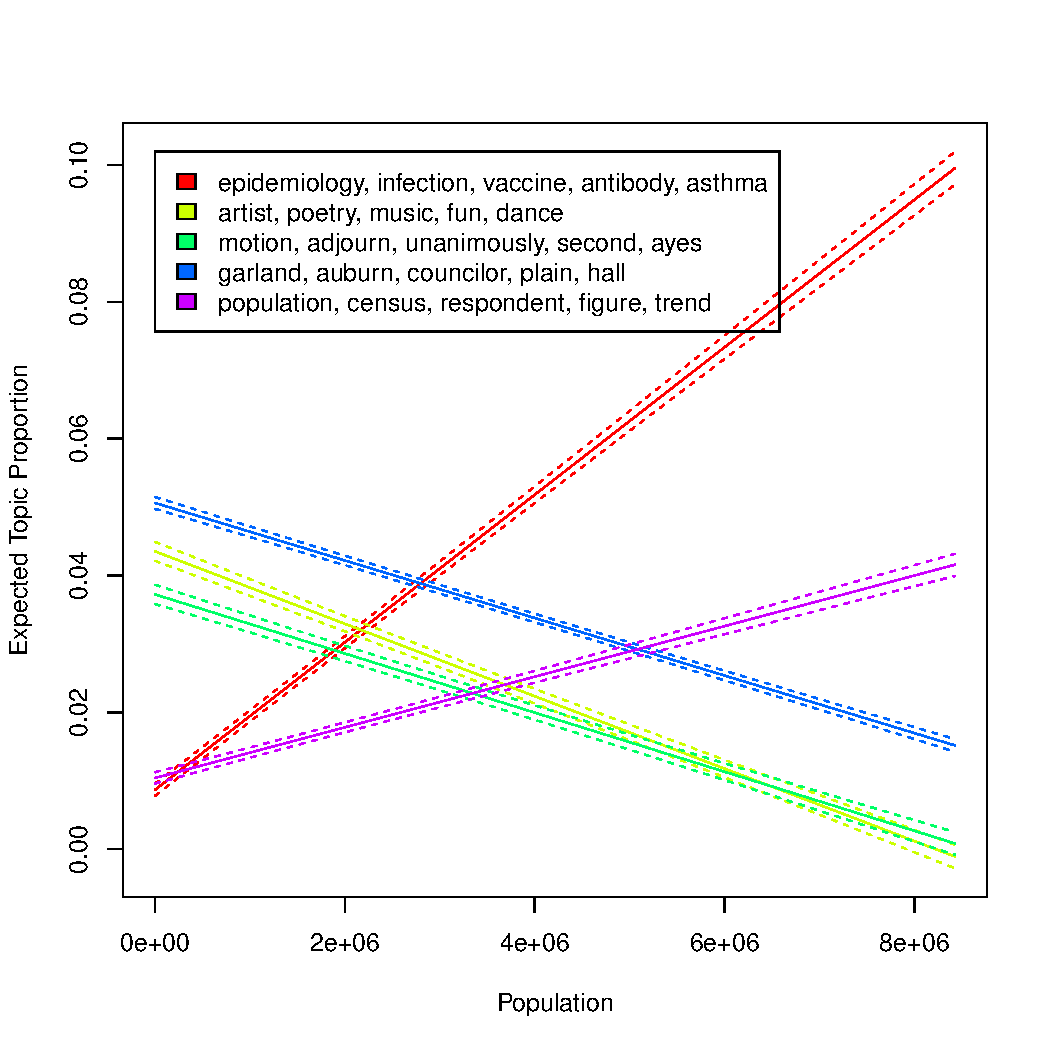
\includegraphics[width=\linewidth]{figures/stm_effect_pop.pdf}
% \end{figure}

% \begin{figure}[htp]
  %  \centering
   % \caption{Five largest topic effects for the median income covariate. The fact that the crime topic is most prevalent in poorer cities, good governance is the most positively correlated with income is indicative of the model's validity.}
   % \label{stmEffectIncome}
    %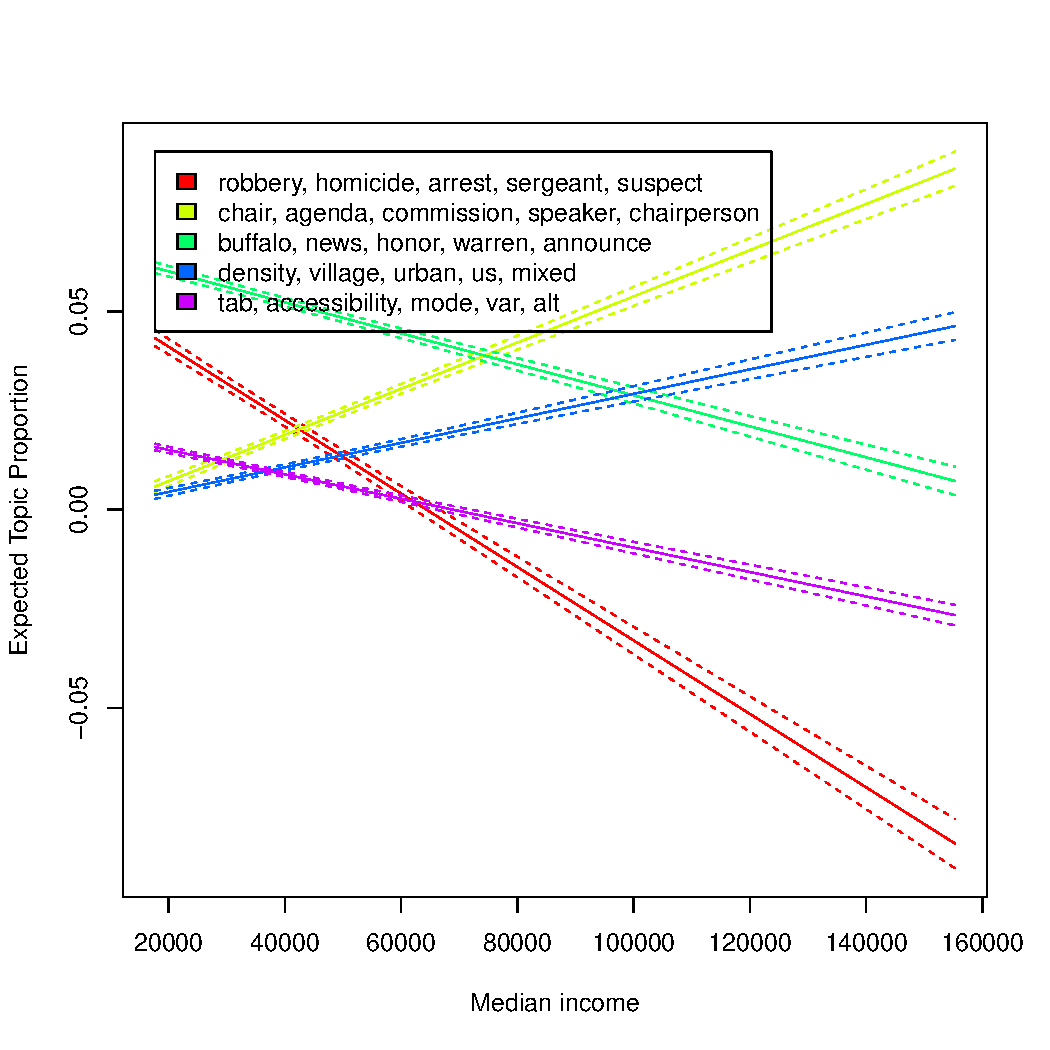
\includegraphics[width=\linewidth]{figures/stm_effect_income.pdf}
%\end{figure}


\end{document}





%\begin{enumerate}
%    \item Design
%    \begin{enumerate}
%        \item Choosing the sample
%        \item Finding URLs
%        \item list of .gov websites
%        \item Finding supporting data
%    \end{enumerate}
%    \item Scraping
%        \begin{enumerate}
%            \item wget
%            \item headless browser/Selenium
%            \item Beautifulsoup/rvest
%            \item APIs (httr)
%            \item Wayback Machine
%        \end{enumerate}
%    \item Pre-processing
%        \begin{enumerate}
%            \item Determining document filetype
%            \item File conversion
%            \item Conventional preprocessing (lowercase, numbers, punctuation)
%            \item Stemming and lemmatization
%            \item spellchecking
%            \item Dealing with duplicate text \& html documents in particular
%        \end{enumerate}
%    \item Analysis
%        \begin{enumerate}
%            \item LDA
%            \item Other topic models (structural, author, dynamic -- maybe?)
%            \item SVM (+ other machine learning classifiers?)
%            \item Fightin Words
%        \end{enumerate}
%\end{enumerate}
%
%
%
%
%
%
%% latex table generated in R 3.3.3 by xtable 1.8-2 package
%% Wed Mar 22 11:32:43 2017
%%\begin{table}[ht]
%%    \centering
%%    \begin{tabular}{lrrlrrl}
%%        \hline
%%        City & DemVotes & RepVotes & Winner & Change & Pop15 & url \\ 
%%        \hline
%%        Attica &  & 187 & Republican & 0 & 3117 & https://attica-in.gov/ \\ 
%%        Connersville & 1005 & 995 & Democratic & 1 & 13010 & http://connersvillecommunity.com/ \\ 
%%        Frankfort &  & 1748 & Republican & 0 & 16060 & http://frankfort-in.gov/ \\ 
%%        Huntingburg & 447 & 793 & Republican & 0 & 6035 & http://www.huntingburg-in.gov/ \\ 
%%        Indianapolis & 92830 & 56661 & Democratic & 1 & 862781 & http://www.indy.gov \\ 
%%        Lake Station & 1483 & 227 & Democratic & 0 & 12054 & http://www.lakestation-in.gov/ \\ 
%%        Linton & 785 & 692 & Democratic & 0 & 5284 & http://www.linton-in.gov/ \\ 
%%        Madison & 1192 & 1915 & Republican & 0 & 12040 & http://www.madison-in.gov/ \\ 
%%        Mitchell & 229 & 495 & Republican & 1 & 4252 & http://mitchell-in.com/ \\ 
%%        Monticello & 0 &  & Democratic & 0 & 5322 & http://www.monticelloin.gov/ \\ 
%%        North Vernon & 679 & 697 & Republican & 1 & 6619 & http://www.northvernon-in.gov/ \\ 
%%        Richmond & 3421 & 2731 & Democratic & 0 & 35854 & http://www.richmondindiana.gov/ \\ 
%%        Rockport & 286 & 272 & Democratic & 1 & 2223 & http://www.cityofrockport-in.gov/ \\ 
%%        South Bend & 8515 & 2074 & Democratic & 0 & 101516 & https://www.southbendin.gov/ \\ 
%%        Union City & 338 & 440 & Republican & 0 & 3447 & http://www.unioncity-in.gov/ \\ 
%%        Winchester & 606 & 524 & Democratic & 1 & 4769 & http://www.winchester-in.gov/ \\ 
%%        \hline
%%    \end{tabular}
%%    \caption{} 
%%\end{table}
%
%\subsection{Research Design}
%
%\begin{table}[ht]
%    \centering
%    \begin{tabular}{llr}
%        \hline
%        Variable & Unit & Source \\
%        \hline
%        Population size & 1000 people & Census \\
%        Population growth last 5 years & Percent & Census \\
%        Type of economy (agriculture/industry/services) & ? & Census \\
%        Economic performance (GDP?) & \$ & Census \\
%        Party of mayor before election & Rep/Dem/(Ind) & in.gov/sos/elections/ \\
%        Party of mayor after election & Rep/Dem/(Ind) & in.gov/sos/elections/ \\
%        Change of party control & 0/1 & in.gov/sos/elections/ \\
%        Presidential vote 2012 in county & Percent Rep & ? (but I have the data) \\
%        Unemployment rate & Percent & Census \\
%        Broadband speed & Avg. Mbps DL & broadbandmap.gov \\
%        \hline
%    \end{tabular}
%    \caption{List of covariates} 
%\end{table}
%
%
%
%\begin{enumerate}
%\item Corpus:
%\begin{enumerate}
%\item Last snapshots before the election (November 3, 2015 in Indiana; tbd. in Louisiana (probably February))
%\item First snapshot that is at least 2 months after the new government's inauguration (which is in January for Indiana, May for Louisiana)
%\end{enumerate}
%\item Preprocessing:
%\begin{enumerate}
%\item restrict corpus to:
%\begin{enumerate}
%\item documents belonging to cities in which a change of power occurred
%\item documents that were added, deleted or changed between the two snapshots
%\end{enumerate}
%\item words to lowercase
%\item remove punctuation
%\item stemming (Porter stemming algorithm?)
%\item Remove stop words (regular list of stop words is enough, since we use an asymmetric prior)
%\end{enumerate}
%\item Apply Grimmer's expressed agenda model to the corpus
%\begin{enumerate}
%\item Asymmetric prior
%\item Each document can have only one topic (in contrast to the author-topic model)
%\item Cities $i = 1,..., n = 15$
%\item Topic $k(k = 1,..., K )$
%\item Documents $j(j = 1,...,D_i)$ from city i
%\item Party covariate in the prior, where the deleted and unmodified documents are coded as from the first, and the added and modified documents from the second party
%\end{enumerate}
%\item Results
%\begin{enumerate}
%\item Label topics using Grimmer's automatic cluster labeling method, based on most commonly used words in documents belonging to topic
%\item Evaluate topics
%\end{enumerate}
%\end{enumerate}
%
%Validation:
%
%\begin{itemize}
%\item Do the above for cities in which no change of power occurred.
%\item Check whether there is higher than average turnover around the new year by comparing changes to non-election years (and also Louisiana, where elections are later).
%\item Check how long documents stay on websites on average. Use websites with a lot of snapshots for this (these exist for both small and large cities).
%\end{itemize}
%
%Problem with using this model: Grimmer's expressed agenda model uses Senators as the actors. Senators is also who he is substantively interested in. For us, the equivalent to Senators is cities. However, we care about parties, not cities.
%
%\subsection{Survival model}
%The existence of individual documents on municipal government websites can be though of as a survival process. No document stays on a website forever, and it appears to be a reasonable assumption that as documents get older and thus less relevant, they get replaced. The factors determining the steepness of the survival curve are the topic - fire safety regulations likely stay up longer than a bulletin on the annual spring banquet - and the change of party control after an election.
%
%\begin{quote}
%\textit{H1}: The older a document, the more likely it is to be removed.
%\end{quote}
%
%$S(t)$ has a downward slope. Admittedly, this is almost impossible not to be true. Also, test proportional, rising and falling hazard models.
%
%\begin{quote}
%\textit{H2}: Documents pertaining to administrative matters are less likely to be removed.
%\end{quote}
%
%Introduce a categorical variable for the top 10(?) topics. A negative coefficient for administrative topics would support this hypothesis.
%
%\begin{quote}
%\textit{H3}: Documents introduced by the opposing party are more likely to be removed.
%\end{quote}
%
%Introduce two variables into the survival model: One variable indicating which party has introduced a document, and a time-varying variable describing which party is currently in government. The hypothesis is tested through an interaction term between the two.
%
%\begin{quote}
%\textit{H4a}: Democrats are more likely to remove documents with topics pertaining to private enterprise, private schools.
%\end{quote}
%
%Interaction term between party in power and categorical topic variable.
%
%\begin{quote}
%\textit{H4b}: Republicans are more likely to remove documents with topics pertaining to social justice, equality, taxes, public schools, etc.
%\end{quote}
%
%Interaction term between party in power and categorical topic variable.
%
%\begin{quote}
%\textit{H5}: In line with their commitment to small government, Republicans are more likely than Democrats to remove documents.
%\end{quote}
%
%Party in power variable.\\
%
%
%This model will take up a lot of degrees of freedom. The rarity of snapshots for some cities might be a problem. Documents being changed and being removed can be modeled as competing risks.
%
%
%\begin{equation} 
%\label{eq1}
%\begin{split}
%Y & = \text{Party that introduced the document} \\
% & + \text{Party that is currently in power} \\
% & + \text{Topic 1, topic 2, ..., topic k} \\
% & + \text{Party that is currently in power} \times \text{Topic 1, topic 2, ..., topic k} \\
% & + \text{Days since start of mayoral term (control)}
%\end{split}
%\end{equation}
%
%
%
%
%
%After the counties, townships and cities that cannot be matched to the Census data\footnote{There are five cities that are not contained in the Census data} and duplicate websites (some cities have more than one website) are removed, 1813 domains/cities remain.
%
%These cities contain 90,616,865 people, and thus about 28\% of the U.S. population (see figure 1).
%
%\begin{figure}[htp]
%    \centering
%    \caption{Percentage of state population covered.}
%    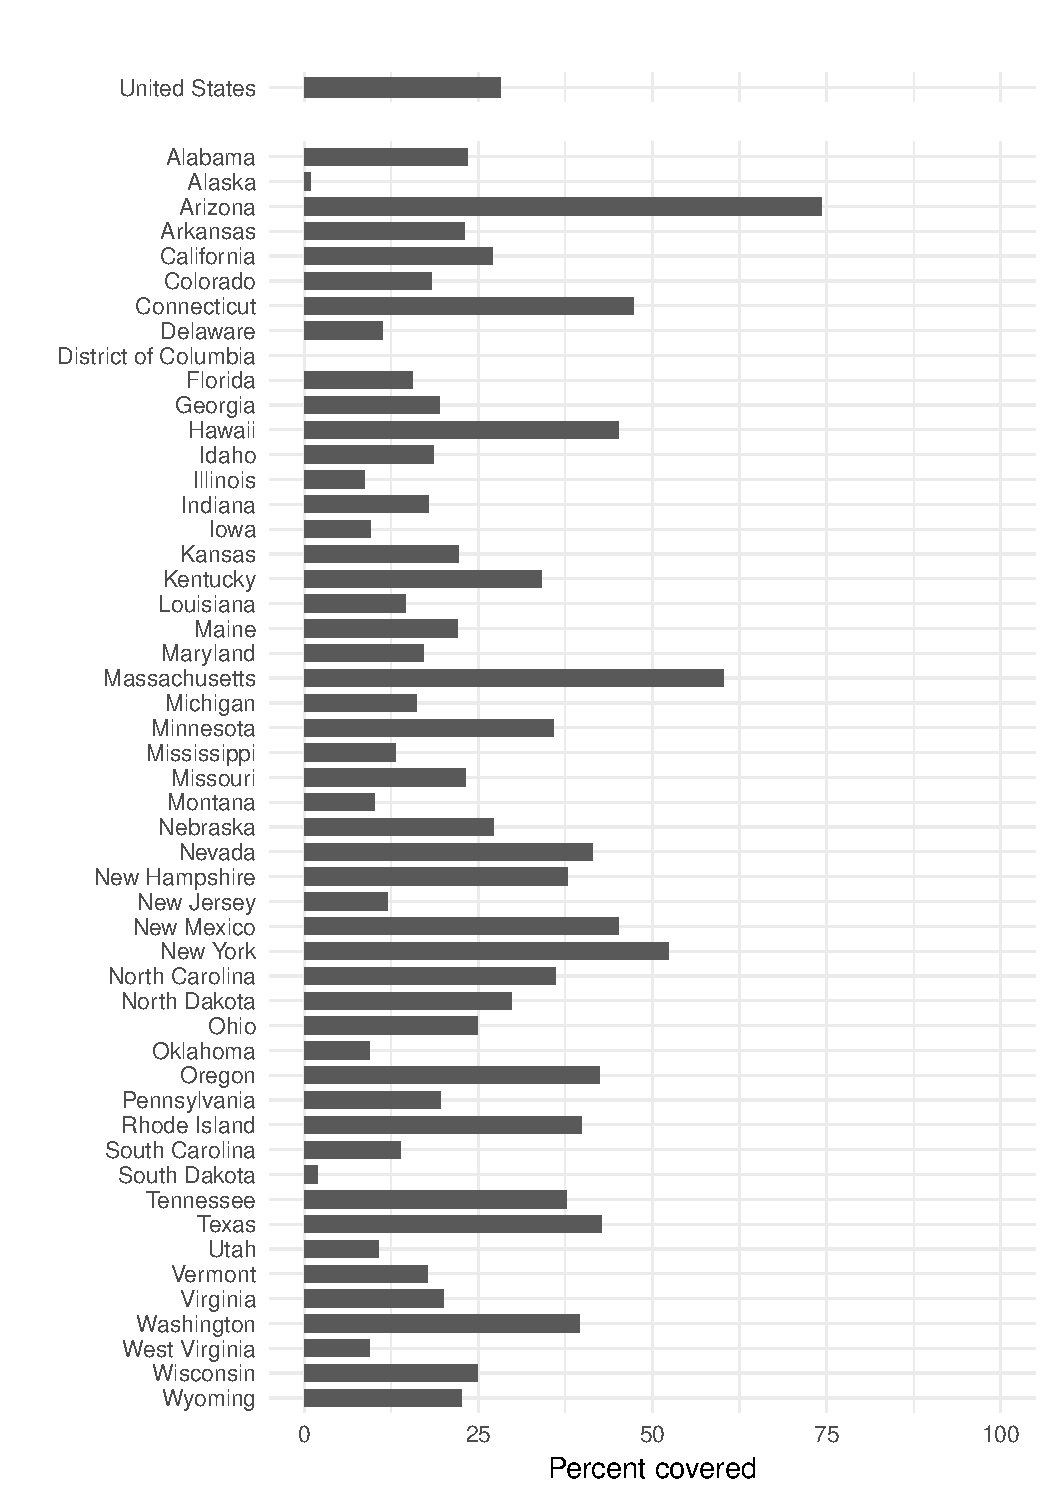
\includegraphics[width=0.9\linewidth,height=0.9\textheight]{figures/coverage_states.pdf}
%\end{figure}
%
%We use the resulting list of websites to acccess their copies stored in the Internet Archive's Wayback Machine. To this end, we rely on the Ruby Gem 'Wayback Machine Downloader'\footnote{https://github.com/hartator/wayback-machine-downloader} (WbMD). We supply the URL that each .gov website redirects to to the WbMD, which then downloads every file present in the WbM from a snapshot in October 2016, or, if not available, as soon as possible after this point.
%
%<Note: We have not actually done this last step for all websites (however, the R script which runs the Ruby package is already set up to do so once we need to). Instead 10 websites were randomly sampled from an older version of the GSA list, which still contained counties and townships, which is why one of the 10 websites is from Dutchess County, NY.>
%
%It would be fine to focus on Indiana as a case. First, we need to answer some preliminary questions about the data.
%
%\begin{enumerate}
%
%\item For what percentage and number of IN cities can we find data from the WBM?
%\item For how many election cycles can we find political leadership data for these matched cities?
%\item In what number and percentage of cities is the local leadership majority Republican? 
%\item Relatedly, in a typical election cycle, for how many cities do we see a transition in party leadership (i.e., a shift from majority D (R) to majority (R) D). 
%
%\end{enumerate}
%
%\begin{enumerate}
%    
%    \item 30 cities, with a combined population of 1,180,435. However, since only cities (as opposed to towns and villages) hold mayoral elections, only 16 of these, with a combined population of 1,094,383 can be matched to the election data.
%    \item 2015, 2011, 2007, 2003.
%    \item Of the 16 cities, 7 have Republican mayors after the 2015 elections.
%    \item In 6 cases, a shift of party control occurs, with 4 of these being Republican --> Democratic. 
%    
%\end{enumerate}
%
%
%
%
%\section{Running Application: Party Differences in Municipal Websites}
%
%
%\begin{landscape}
%\begin{table}[htbp]
%    %\caption{}
%    \begin{tabular}{|p{2cm}|c|p{3cm}|p{12cm}|l|}
%        \hline
%        Names & Year & Journal & Findings & Important? \\ \hline
%        Benedictis-Kessner, Justin De
%        Warshaw, Christopher & 2016 & JOP* & Regression discontinuity design. Democratic mayors spend more (but it is unclear on what, not the typical Democratic issue-areas), issue more debt, pay more interest & Yes \\ \hline
%        Caughey, Devin
%        Warshaw, Christopher
%        Xu, Yiqing & 2015 & Working Paper & Regression discontinuity design. Partisan composition of state governments affects state policy liberalism (composite index for the areas of social welfare, taxation, labor, civil rights, women’s rights, moral legislation, family planning, environment). & Somewhat \\ \hline
%        Einstein, Katherine Levine
%        Kogan, Vladimir & 2015 & Urban Affairs Review & Cities with more Democratic citizens spend more; more progressive (rather than regressive) forms of taxation; pursue intergov. aid more; spend more on police, fire, parks \& recreation & Somewhat \\ \hline
%        Einstein, Katherine Levine
%        Glick, David M. & 2015 & Working Paper & Survey of 72 mayors. Unlike Republican mayors, roughly half of Democrats seem to agree that cities should aim to reduce inequality. Democratic mayors also seem to favor redistribution to accomplish that goal. & Somewhat \\ \hline
%        Kiewiet, D Roderick
%        Mccubbins, Mathew D & 2014 & Annual Review & City budgets have been severeley constrained since the Great Recession. Spending has thus decreased in general. Lack of funds means that there is not much discretion for partisanship. & Somewhat \\ \hline
%        Tausanovitch, Chris
%        Warshaw, Christopher & 2014 & APSR* & Cities are responsive (taxes, expenditures, regressiveness of taxation) to citizens' conservatism/liberalism. Partisan elections do not make cities more or less responsive. & Yes \\ \hline
%        Guillamón, Ma Dolores
%        Bastida, Francisco
%        Benito, Bernardino & 2013 & European Journal of Law and Economics & Police spending in Spain. Conservative parties spend more on police. Spending is higher before elections. Also contains a useful overview of the literature. & Yes \\ \hline
%    \end{tabular}
%    \label{}
%\end{table}
%\end{landscape}
%
%\begin{landscape}
%    \begin{table}[htbp]
%        %\caption{}
%        \begin{tabular}{|p{2cm}|c|p{3cm}|p{12cm}|l|}
%            \hline
%            Names & Year & Journal & Findings & Important? \\ \hline
%            Gerber, Elisabeth R. & 2013 & Cityscape & Partisanship of both citizens and elected city officials separately affect climate policy. & Yes \\ \hline
%            Solé-Ollé, Albert
%            Viladecans-Marsal, Elisabet & 2013 & Journal of Urban Economics & Spanish cities. The authors "employ a regression discontinuity design to document that cities controlled by left-wing parties convert much less land from rural to urban uses than is the case in similar cities con- trolled by the right". Partisanship might also affect housing construction and price growth. & Yes \\ \hline
%            Gerber, Elisabeth R.
%            Hopkins, Daniel J. & 2011 & AJPS & Regression discontinuity design. Democratic mayors spend less on public safety. All other policy areas (including taxation) are unaffected. & Yes \\ \hline
%            Trounstine, Jessica & 2010 & Annual Review & Race and ethnicity in local elections (not relevant to us). Partisan elections have higher turnout; non-partisan elections still tend to have some partisanship in them because voters learn about party of candidates from media. Non-partisan elections favor Republicans/upper class. Mixed evidence for whether partisanship of mayor is important for policy. & Somewhat \\ \hline
%            Palus, Christine Kelleher & 2010 & State and Local Government Review & Ideology (liberal/conservative) of citizen is well represented by gov. spending in five areas: (1) community development, housing, and conservation, (2) health and human services, (3) culture, the arts, and recreation, (4) environmental programs, and (5) transportation. & Somewhat \\ \hline
%            Ferreira, Fernando
%            Gyourko, Joseph & 2009 & The Quarterly Journal of Economics & Regression discontinuity design. Null results for spending and city gov. size with regard to mayor partisanship. & Yes \\ \hline
%            Ansolabehere, Stephen
%            Snyder, James M. & 2006 & Scandinavian Journal of Economics & Despite the journal, this is about the U.S. The important finding (for us) is the fact that counties whose government is controlled by the same party as the state government, receive more funding (county's share of state transfers, normalized by county pop.) from the state. & Somewhat \\ \hline
%            Murphy, Russell D. & 2002 & Annual Review & Not useful. Too philosophical; mostly cites papers written a hundred years ago. Also exclusively about larger cities. & No \\ \hline
%        \end{tabular}
%        \label{}
%    \end{table}
%\end{landscape}
%
%\begin{landscape}
%    \begin{table}[htbp]
%        %\caption{}
%        \begin{tabular}{|p{2cm}|c|p{3cm}|p{12cm}|l|}
%            \hline
%            Names & Year & Journal & Findings & Important? \\ \hline
%            Armstrong, Cory L. & 2011 & Government Information Quarterly & Comparison of county and school board websites in Florida (where the two align) with regard to transparency (presence or absence of public records). Manual content analysis (undergrads told to look around for 15 minutes). School board websites, more professional websites, and websites in Republican-dominated counties are found to be more transparent. & Yes \\ \hline
%            Cegarra-Navarro, Juan
%            Pachón, José
%            Cegarra, José & 2012 & International Journal of Information Management & Survey of Spanish municipal government officials (specifically, the city website managers). Respondents are asked about the features of their websites, the level of civic engagement and the size of their municipality. More sophisticated websites are correlated with greater civic engagement and greater use of e-government functions. & Yes \\ \hline
%            Dolson, Jordan
%            Young, Robert & 2012 & Canadian Journal of Urban Research & Determinants of website content. Three categories: e-content (city information on website), e-participation, social media use. Tables on page 15 show frequencies of these categories across sites, and might be useful to inform our topics. Larger cities have better websites. Population growth and immigration are also tested, but the findings are somewhat inconclusive. & Yes \\ \hline
%            Feeney, Mary K.
%            Brown, Adrian & 2017 & Government Information Quarterly & 500 U.S. city websites at two points in time (2010-2014). Count model of website features regarding information, e-services, utilities, transparency and civic engagement. Having a larger population leads to more features. Relying on a website contractor leads to more information and transparency. The authors say that mayor-councils are negatively correlated with website sophistication, but their regression tables state the opposite. & Yes \\ \hline
%            Kaylor, Charles
%            Deshazo, Randy
%            Van Eck, David & 2001 & Government Information Quarterly & Model of best practices of e-government. Table 1 lists a number of possible ways this manifests, could be useful for our theory. & Somewhat \\ \hline
%            Ansolabehere, Stephen
%            Urban, Florian & 2002 & Cities & Websites of 20 major cities across the world. Is website content correlated with city characteristics? Not particularly systematic, and the findings are inconclusive. & Somewhat \\ \hline
%            Jeffres, Leo W.
%            Lin, Carolyn A. & 2006 & Journal of Computer-Mediated Communication & 50 largest metropolitan areas in the U.S. Features include information about city, opportunities for citizen feedback, galleries of photos, links, etc.  Purely descriptive analysis, doesn't contain anything that isn't covered in any of the other aricles. & No \\ \hline
%        \end{tabular}
%        \label{}
%    \end{table}
%\end{landscape}
%
%\subsection{Informative Dirichlet model}
%%However, \cite{Monroe2008} advise against using these types of methods in this context because they get the data generation process backwards: Our theory assumes that party leads to variation in writing, and yet we rely on the documents to predict party, in spite of the fact that we actually have perfect knowledge of it.
%
%For the analysis of the data, we present two approaches, the first being the informative dirichlet model developed by \citep{Monroe2008}. This approach aims to account for the fact that some words naturally occur more than others by applying a Dirichlet prior based on the distribution of words in random text. Table \ref{tabFightinIN} shows the top words for both Democrats and Republicans - and accomplishes, to some extent, the goal of \citep{Monroe2008} of banishing frequent words from this list and supplanting them with text with greater semantic, and in our case, partisan meaning. 
%
%In Indiana, Democrats exhibit a preference for words related to public finance, such as 'fund', 'budget', or 'tax', indicative of a greater willingness to emphasize the city's efforts to raise and spend money. This finding is consistent with \citep{Einstein2015}, who show that Democratic mayors tend to favor greater spending. Beyond the focus on public finance, the words preferably used by Democrats do not fall into any particularly congruent categories, and largely sort into various areas related to city administration - i.e. `council', `services', `budget', `committee', `contract', etc. If there is theme around the words preferred by Republicans, it seems to center around city planning - street, fire, water, building, construction, park. These words suggest that the hands-off approach favored by Republicans results in a focus on supporting infrastructure and logistics.
%
%%Partisan top words - fightin words Indiana
%% latex table generated in R 3.4.1 by xtable 1.8-2 package
% Fri Oct 20 10:49:17 2017
\begin{table}[ht]
\centering
\begingroup\fontsize{9pt}{10pt}\selectfont
\begin{tabular}{lrlr}
  \hline
Word (D) & z-Score (D) & Word (R) & z-Score (R) \\ 
  \hline
said & 86.20 & request & 69.41 \\ 
  proposal & 70.98 & member & 67.45 \\ 
  fund & 59.22 & street & 47.84 \\ 
  county & 54.15 & motion & 46.35 \\ 
  asked & 52.62 & councilor & 45.69 \\ 
  budget & 49.40 & main & 44.34 \\ 
  stated & 46.90 & goods & 44.33 \\ 
  tax & 41.79 & use & 43.43 \\ 
  fort & 41.17 & tree & 42.77 \\ 
  ms & 40.76 & amp & 42.48 \\ 
  division & 38.01 & water & 41.45 \\ 
  million & 36.62 & downtown & 40.66 \\ 
  grants & 35.21 & pm & 39.60 \\ 
  introduced & 34.85 & sign & 39.28 \\ 
  contract & 34.36 & st & 38.23 \\ 
  revenue & 34.33 & plan & 38.20 \\ 
  general & 34.17 & rd & 37.71 \\ 
  chair & 32.01 & site & 37.19 \\ 
  brown & 31.86 & docket & 37.03 \\ 
  federal & 31.46 & trees & 36.56 \\ 
  metropolitan & 31.25 & plat & 36.15 \\ 
  management & 30.69 & old & 35.44 \\ 
  agency & 30.35 & residential & 34.65 \\ 
  approves & 29.66 & area & 34.31 \\ 
  authorizes & 29.11 & variance & 33.50 \\ 
  technology & 28.45 & th & 33.20 \\ 
  provide & 27.43 & utility & 33.11 \\ 
  dollars & 27.30 & ordinance & 32.04 \\ 
  consolidated & 26.29 & carter & 31.40 \\ 
  justice & 25.93 & approve & 31.40 \\ 
  parks & 25.79 & building & 30.78 \\ 
  lewis & 25.73 & feet & 30.16 \\ 
  increase & 25.66 & news & 29.37 \\ 
  digest & 25.60 & city & 29.26 \\ 
  support & 25.43 & lots & 29.19 \\ 
  oliver & 25.43 & lot & 28.89 \\ 
  animal & 25.02 & aid & 28.54 \\ 
  gray & 24.72 & overlay & 28.53 \\ 
  capital & 24.54 & home & 28.52 \\ 
  services & 24.53 & democrat & 28.40 \\ 
  amends & 23.84 & republican & 28.25 \\ 
  criminal & 23.70 & uses & 28.05 \\ 
  enterprise & 23.62 & must & 27.57 \\ 
  mayors & 23.51 & legal & 26.64 \\ 
  court & 22.90 & zoning & 26.53 \\ 
  township & 22.86 & councilors & 26.50 \\ 
  controls & 22.54 & river & 26.48 \\ 
  funded & 22.28 & stellar & 26.40 \\ 
  referred & 22.16 & common & 26.15 \\ 
  fiscal & 22.10 & rep & 26.03 \\ 
   \hline
\end{tabular}
\endgroup
\caption{Top 50 democratic and Republican words (Indiana), according to the informed 
             Dirichlet model of Monroe et al. (2008).} 
\label{tabFightinIN}
\end{table}

 %\ref{tabFightinIN}
%
%For Lousiana, the results (see table \ref{tabFightinLA}) are less coherent. Only one of the finance-related terms appears again for Democrats - specifically `fund', although `rate' might also be used in a financial context. Beyond that, some focus on a `historic' `'district of a city seems evident, as is the use of some words - `infrastructure', `water', `building' that were used for Republicans in Indiana. Conversely, Republicans are now missing these words, and their preferred terms generally do not seem to follow any particular theme.
%
%%Partisan top words - fightin words Louisiana
%% latex table generated in R 3.4.3 by xtable 1.8-2 package
% Tue Dec 26 15:00:39 2017
\begin{table}[ht]
\centering
\begingroup\fontsize{9pt}{10pt}\selectfont
\begin{tabular}{lrlr}
  \hline
Word (D) & z-Score (D) & Word (R) & z-Score (R) \\ 
  \hline
otherwise & 20.73 & say & 86.18 \\ 
  health & 18.65 & ordinance & 77.67 \\ 
  respect & 17.98 & summary & 59.81 \\ 
  use & 16.62 & bid & 58.98 \\ 
  officer & 16.22 & council & 46.92 \\ 
  staff & 15.87 & amount & 41.21 \\ 
  district & 15.82 & official & 39.79 \\ 
  historic & 15.51 & mayor & 39.07 \\ 
  datum & 15.19 & accordance & 37.91 \\ 
  fund & 15.02 & boulevard & 37.78 \\ 
  thereto & 14.86 & weekend & 35.41 \\ 
  building & 14.70 & weather & 34.34 \\ 
  street & 14.69 & seal & 33.27 \\ 
  total & 14.60 & responsive & 33.15 \\ 
  window & 14.50 & veteran & 31.96 \\ 
  applicant & 14.41 & resolution & 29.52 \\ 
  exist & 14.19 & hold & 28.71 \\ 
  housing & 14.13 & gathering & 28.32 \\ 
  provide & 13.84 & furnish & 27.36 \\ 
  review & 13.58 & councilman & 27.19 \\ 
  source & 13.54 & meeting & 26.74 \\ 
  neighborhood & 13.09 & exceed & 26.54 \\ 
  revenue & 12.99 & show & 26.44 \\ 
  target & 12.88 & emergency & 26.01 \\ 
  policy & 12.75 & resident & 25.23 \\ 
  training & 12.52 & city & 24.89 \\ 
  process & 12.51 & accept & 24.73 \\ 
  actual & 12.45 & visit & 24.67 \\ 
  population & 12.04 & wheeler & 24.21 \\ 
  green & 11.95 & night & 24.11 \\ 
  rate & 11.70 & purchase & 24.00 \\ 
  infrastructure & 11.68 & theater & 23.76 \\ 
  urban & 11.46 & parish & 23.63 \\ 
  average & 11.45 & sweep & 23.39 \\ 
  retention & 11.22 & inc & 23.27 \\ 
  master & 11.03 & tonight & 22.09 \\ 
  bureau & 10.93 & recreation & 21.92 \\ 
  roof & 10.90 & mike & 21.82 \\ 
  strategy & 10.89 & park & 21.78 \\ 
  water & 10.82 & department & 21.71 \\ 
  construct & 10.79 & movie & 21.65 \\ 
  residence & 10.57 & tropical & 21.50 \\ 
  reduce & 10.47 & hall & 21.49 \\ 
  relative & 10.46 & contract & 21.31 \\ 
  construction & 10.46 & pet & 21.24 \\ 
  monthly & 10.46 & morning & 21.08 \\ 
  chapter & 10.43 & begin & 20.84 \\ 
  individual & 10.35 & information & 20.78 \\ 
  design & 10.29 & beach & 20.60 \\ 
  standard & 10.24 & approve & 20.56 \\ 
   \hline
\end{tabular}
\endgroup
\caption{Top 50 Democratic and Republican words (Louisiana), according to the informed Dirichlet model of Monroe et al. (2008).} 
\label{tabFightinLA}
\end{table}

 %\ref{tabFightinLA}
%
%The weakness of the fightin' words method is evident here, as a list of words does not necessarily provide sufficient information to glean preferred topics from. This is especially the case when the texts are spread across a broad number of issue-areas, with little semantic similarity. In \citep{Monroe2008}, the authors focus on the fairly constrained corpus of U.S. Senate speeches with respect to abortion - our context, by comparison, is far more eclectic.








